\chapter{Appendix: Detailed Metrics Reporting}\label{appendixA}


\section{Dataset-Specific Models}

\subsection{Weather}


\begin{table}[h!]
     \centering
     \begin{tabular}{lcccc}
     \hline
     Model & RMSE  & MAE   & MAPE  & R2 Score \\
     \hline
     SAMFormer   & 0.4065 & 0.3308 & 1.1723 & 0.7928 \\
     TimesFM     & 0.4282 & 0.3398 & 1.0393 & 0.7725 \\
     TimeGPT     & 0.1475 & 0.1232 & 2.5538 & 0.0776 \\
     Time-MoE    & 0.4824 & 0.3819 & 1.5142 & 0.7825 \\
     \hline
     \end{tabular}
     \caption{Deep Learning Models for Horizon 64 $\to$ 32}
     \label{tab:weather_64to32_dl}
\end{table}
     

\begin{table}[h!]
     \centering
     \begin{tabular}{lrr}
     \hline
     Model                       & MAE   & RMSE  \\
     \hline
     LinearRegression            & 0.2947 & 0.3673 \\
     RandomForestRegressor       & 0.3228 & 0.4099 \\
     ExtraTreesRegressor         & 0.3098 & 0.3980 \\
     MLPRegressor                & 0.3615 & 0.4488 \\
     Linear SVR                  & 0.4013 & 0.4954 \\
     HistGradientBoostingRegressor & 0.3875 & 0.4817 \\
     \hline
     \end{tabular}
     \caption{Regressor Models for Horizon 64 $\to$ 32}
     \label{tab:weather_64to32_reg}
\end{table}
     


\begin{table}[h!]
     \centering
     \begin{tabular}{lcccc}
     \hline
     Model & RMSE  & MAE   & MAPE  & R2 Score \\
     \hline
     SAMFormer   & 0.4754 & 0.3773 & 1.1654 & 0.7056 \\
     TimesFM     & 0.4410 & 0.3514 & 1.3885 & 0.6432 \\
     TimeGPT     & 0.4390 & 0.3312 & 1.6603 & -0.3999 \\
     Time-MoE    & 0.4536 & 0.3548 & 1.4598 & 0.7137 \\
     \hline
     \end{tabular}
     \caption{Deep Learning Models for Horizon 128 $\to$ 64}
     \label{tab:weather_128to64_dl}
\end{table}
     

\begin{table}[h!]
     \centering
     \begin{tabular}{lcc}
     \hline
     Model & MAE   & RMSE  \\
     \hline
     LinearRegression                & 0.2989 & 0.3767 \\
     RandomForestRegressor           & 0.3167 & 0.3881 \\
     ExtraTreesRegressor             & 0.3122 & 0.3824 \\
     MLPRegressor                    & 0.3519 & 0.4358 \\
     Linear SVR                      & 0.3869 & 0.4745 \\
     HistGradientBoostingRegressor   & 0.3564 & 0.4507 \\
     \hline
     \end{tabular}
     \caption{Regressor Models for Horizon 128 $\to$ 64}
     \label{tab:weather_128to64_reg}
\end{table}
     


\begin{table}[h!]
     \centering
     \begin{tabular}{lcccc}
     \hline
     Model & RMSE  & MAE   & MAPE  & R2 Score \\
     \hline
     SAMFormer   & 0.4058 & 0.3308 & 1.1723 & 0.7928 \\
     TimesFM     & 0.3883 & 0.3072 & 1.2693 & 0.7552 \\
     TimeGPT     & 0.3883 & 0.3072 & 1.2693 & 0.7552 \\
     Time-MoE    & 1.1019 & 0.9386 & 2.0021 & -0.4937 \\
     \hline
     \end{tabular}
     \caption{Deep Learning Models for Horizon 256 $\to$ 128}
     \label{tab:weather_256to128_dl}
\end{table}
     

\begin{table}[h!]
     \centering
     \begin{tabular}{lcc}
     \hline
     Model & MAE & RMSE \\
     \hline
     LinearRegression              & 0.4098 & 0.5097 \\
     RandomForestRegressor         & 0.2948 & 0.3619 \\
     ExtraTreesRegressor           & 0.2889 & 0.3565 \\
     MLPRegressor                  & 0.3660 & 0.4531 \\
     Linear SVR                    & 0.4189 & 0.5136 \\
     HistGradientBoostingRegressor & 0.4038 & 0.5158 \\
     \hline
     \end{tabular}
     \caption{Regressor Models for Horizon 256 $\to$ 128}
     \label{tab:regressors_256to128}
\end{table}
     




\newpage
\subsection{Finance}

\begin{table}[h!]
\centering
\begin{tabular}{lcccc}
\hline
Model & RMSE (manual) & MAE & MAPE & R2 Score \\
\hline
SAMFormer   & 1.2537 & 0.8397 & 0.07415 & 0.9830 \\
TimesFM     & 1.7423 & 1.2073 & 0.0995  & 0.9662 \\
TimeGPT     & 0.0197 & 0.0174 & 0.0450  & -0.0164 \\
Time-MoE    & 0.1728 & 0.1121 & 0.9602  & 0.9680 \\
\hline
\end{tabular}
\caption{Deep Learning Models for Horizon 64 \texorpdfstring{$\to$}{->} 32}
\label{tab:finance_64to32_dl}
\end{table}

\begin{table}[h!]
\centering
\begin{tabular}{lccc}
\hline
Model & MAE & RMSE \\
\hline
LinearRegression              & 0.1253 & 0.1738 \\
RandomForestRegressor         & 1.2835 & 1.6653 \\
ExtraTreesRegressor           & 1.2869 & 1.6682 \\
MLPRegressor                  & 1.0366 & 1.5134 \\
Linear SVR                    & 0.1520 & 0.2083 \\
HistGradientBoostingRegressor & 1.3442 & 1.7122 \\
\hline
\end{tabular}
\caption{Regressor Models for Horizon 64 \texorpdfstring{$\to$}{->} 32}
\label{tab:finance_64to32_reg}
\end{table}

\begin{table}[h!]
\centering
\begin{tabular}{lcccc}
\hline
Model & RMSE & MAE & MAPE & R2 Score \\
\hline
SAMFormer   & 1.7918 & 1.2279 & 0.10377 & 0.9638 \\
TimesFM     & 2.2162 & 1.5125 & 0.1315  & 0.9420 \\
TimeGPT     & 0.0158 & 0.0132 & 0.0340  & -0.1067 \\
Time-MoE    & 0.2136 & 0.1446 & 1.1279  & 0.9482 \\
\hline
\end{tabular}
\caption{Deep Learning Models for Horizon 128 \texorpdfstring{$\to$}{->} 64}
\label{tab:finance_128to64_dl}
\end{table}

\begin{table}[h!]
\centering
\begin{tabular}{lcccc}
\hline
Model & MAE & RMSE \\
\hline
LinearRegression              & 0.2089 & 0.2849 \\
RandomForestRegressor         & 1.3105 & 1.6671 \\
ExtraTreesRegressor           & 1.3038 & 1.6618 \\
MLPRegressor                  & 1.1546 & 1.6571 \\
Linear SVR                    & 0.2444 & 0.3315 \\
HistGradientBoostingRegressor & 1.3361 & 1.6863 \\
\hline
\end{tabular}
\caption{Regressor Models for Horizon 128 \texorpdfstring{$\to$}{->} 64}
\label{tab:finance_128to64_reg}
\end{table}

\begin{table}[h!]
\centering
\begin{tabular}{lcccc}
\hline
Model & RMSE & MAE & MAPE & R2 Score \\
\hline
SAMFormer   & 2.4161 & 1.6667 & 0.13844 & 0.9288 \\
TimesFM     & 2.9006 & 2.0680 & 0.1502  & 0.8874 \\
TimeGPT     & 0.0662 & 0.0416 & 0.1500  & -0.4434 \\
Time-MoE    & 0.9568 & 0.7537 & 2.9146  & -0.1791 \\
\hline
\end{tabular}
\caption{Deep Learning Models for Horizon 256 \texorpdfstring{$\to$}{->} 128}
\label{tab:finance_256to128_dl}
\end{table}

\begin{table}[h!]
\centering
\begin{tabular}{lcccc}
\hline
Model & MAE & RMSE \\
\hline
LinearRegression              & 0.3486 & 0.4572 \\
RandomForestRegressor         & 1.3564 & 1.6762 \\
ExtraTreesRegressor           & 1.3494 & 1.6702 \\
MLPRegressor                  & 1.1109 & 1.5923 \\
Linear SVR                    & 0.3652 & 0.4795 \\
HistGradientBoostingRegressor & 1.3756 & 1.6902 \\
\hline
\end{tabular}
\caption{Regressor Models for Horizon 256 \texorpdfstring{$\to$}{->} 128}
\label{tab:finance_256to128_reg}
\end{table}
\subsection{Energy}

\begin{table}[h!]
\centering
\begin{tabular}{lcccc}
\hline
Model & RMSE & MAE & MAPE & R2 Score \\
\hline
SAMFormer   & 0.54167 & 0.30328 & 0.64230 & 0.64452 \\
TimesFM     & 0.5790  & 0.34330 & 0.75740 & 0.58670 \\
TimeGPT     & 1.6972  & 1.36710 & 4.50990 & -1.62520 \\
Time-MoE    & 0.80567 & 0.45576 & 0.72627 & 0.35959 \\
\hline
\end{tabular}
\caption{Deep Learning Models for Energy, Horizon 64 \texorpdfstring{$\to$}{->} 32}
\label{tab:energy_64to32_dl}
\end{table}

\begin{table}[h!]
\centering
\begin{tabular}{lcccc}
\hline
Model & MAE & RMSE \\\hline
LinearRegression              & 0.5014 & 0.6978 \\
RandomForestRegressor         & 0.3157 & 0.5860 \\
ExtraTreesRegressor           & 0.3050 & 0.5598 \\
MLPRegressor                  & 0.3933 & 0.5936 \\
Linear SVR                    & 0.7456 & 0.9987 \\
HistGradientBoostingRegressor & 0.4549 & 0.6248 \\
\hline
\end{tabular}
\caption{Regressor Models for Energy, Horizon 64 \texorpdfstring{$\to$}{->} 32}
\label{tab:energy_64to32_reg}
\end{table}

\begin{table}[h!]
\centering
\begin{tabular}{lcccc}
\hline
Model & RMSE & MAE & MAPE & R2 Score \\
\hline
SAMFormer   & 0.54040 & 0.29871 & 0.63941 & 0.64619 \\
TimesFM     & 0.5620  & 0.33460 & 0.74670 & 0.61800 \\
TimeGPT     & 1.7757  & 1.53210 & 4.65720 & -2.76040 \\
Time-MoE    & 0.62323 & 0.34837 & 0.62219 & 0.62399 \\
\hline
\end{tabular}
\caption{Deep Learning Models for Energy, Horizon 128 \texorpdfstring{$\to$}{->} 64}
\label{tab:energy_128to64_dl}
\end{table}

\begin{table}[h!]
\centering
\begin{tabular}{lcccc}
\hline
Model & MAE & RMSE \\
\hline
LinearRegression              & 0.4136 & 0.6287 \\
RandomForestRegressor         & 0.2914 & 0.5545 \\
ExtraTreesRegressor           & 0.2848 & 0.5456 \\
MLPRegressor                  & 0.3599 & 0.5581 \\
Linear SVR                    & 0.6760 & 0.9015 \\
HistGradientBoostingRegressor & 0.4134 & 0.5901 \\
\hline
\end{tabular}
\caption{Regressor Models for Energy, Horizon 128 \texorpdfstring{$\to$}{->} 64}
\label{tab:energy_128to64_reg}
\end{table}

\begin{table}[h!]
\centering
\begin{tabular}{lcccc}
\hline
Model & RMSE & MAE & MAPE & R2 Score \\
\hline
SAMFormer   & 0.54043 & 0.29924 & 0.64137 & 0.64613 \\
TimesFM     & 0.8225  & 0.55930 & 0.91270 & 0.19990 \\
TimeGPT     & 1.8662  & 1.65420 & 5.31130 & -2.91740 \\
Time-MoE    & 1.08894 & 0.83396 & 1.20268 & -0.12809 \\
\hline
\end{tabular}
\caption{Deep Learning Models for Energy, Horizon 256 \texorpdfstring{$\to$}{->} 128}
\label{tab:energy_256to128_dl}
\end{table}

\begin{table}[h!]
\centering
\begin{tabular}{lcccc}
\hline
Model & MAE & RMSE \\\hline
LinearRegression              & 0.3273 & 0.5551 \\
RandomForestRegressor         & 0.2948 & 0.5647 \\
ExtraTreesRegressor           & 0.2880 & 0.5616 \\
MLPRegressor                  & 0.3656 & 0.5747 \\
Linear SVR                    & 0.5653 & 0.7760 \\
HistGradientBoostingRegressor & 0.4036 & 0.5942 \\
\hline
\end{tabular}
\caption{Regressor Models for Energy, Horizon 256 \texorpdfstring{$\to$}{->} 128}
\label{tab:energy_256to128_reg}
\end{table}
\newpage
\subsection{Healthcare}

\begin{table}[h!]
\centering
\begin{tabular}{lcccc}
\hline
Model & RMSE & MAE & MAPE & R2 Score \\
\hline
SAMFormer & 1.0920 & 0.7214 & 8.7253 & -1.2159 \\
TimesFM   & 0.5160 & 0.3676 & 4.8562 & 0.2721 \\
TimeGPT   & 2.9776 & 2.3762 & 0.9697 & -17.0530 \\
Time-MoE  & 0.3286 & 0.2179 & 1.7545 & 0.6273 \\
\hline
\end{tabular}
\caption{Deep Learning Models for Healthcare, Horizon 64 \texorpdfstring{$\to$}{->} 32}
\label{tab:healthcare_64to32_dl}
\end{table}

\begin{table}[h!]
\centering
\begin{tabular}{lcccc}
\hline
Model & MAE & RMSE \\\hline
LinearRegression              & 0.7121 & 1.0847 \\
RandomForestRegressor         & 1.8881 & 2.0738 \\
ExtraTreesRegressor           & 1.6375 & 1.7732 \\
MLPRegressor                  & 1.0811 & 1.5152 \\
Linear SVR                    & 0.9266 & 1.4208 \\
HistGradientBoostingRegressor & 1.1408 & 1.2652 \\
\hline
\end{tabular}
\caption{Regressor Models for Healthcare, Horizon 64 \texorpdfstring{$\to$}{->} 32}
\label{tab:healthcare_64to32_reg}
\end{table}

\begin{table}[h!]
\centering
\begin{tabular}{lcccc}
\hline
Model & RMSE & MAE & MAPE & R2 Score \\
\hline
SAMFormer & 2.3210 & 1.78826 & 20.97415 & -16.42980 \\
TimesFM   & 0.8537 & 0.65110 & 10.18890 & -1.94810 \\
TimeGPT   & 5.9754 & 5.06290 & 5.24600  & -24.00790 \\
Time-MoE  & 0.50288& 0.39035 & 1.04249  & -0.28967 \\
\hline
\end{tabular}
\caption{Deep Learning Models for Healthcare, Horizon 128 \texorpdfstring{$\to$}{->} 64}
\label{tab:healthcare_128to64_dl}
\end{table}

\begin{table}[h!]
\centering
\begin{tabular}{lcccc}
\hline
Model & MAE & RMSE \\\hline
LinearRegression              & 2.3868 & 3.1923 \\
RandomForestRegressor         & 1.9649 & 2.1291 \\
ExtraTreesRegressor           & 1.8989 & 2.0403 \\
MLPRegressor                  & 0.7829 & 1.0326 \\
Linear SVR                    & 2.1916 & 3.0589 \\
HistGradientBoostingRegressor & 1.3243 & 1.4157 \\
\hline
\end{tabular}
\caption{Regressor Models for Healthcare, Horizon 128 \texorpdfstring{$\to$}{->} 64}
\label{tab:healthcare_128to64_reg}
\end{table}

\begin{table}[h!]
\centering
\begin{tabular}{lcccc}
\hline
Model & RMSE & MAE & MAPE & R2 Score \\
\hline
SAMFormer & 8.45283 & 7.05131 & 99.87629 & -316.1960 \\
TimesFM   & 8.7030  & 6.3970  & 20.74610 & -1930.9374 \\
TimeGPT   & 11.1004 & 9.7487  & 55.82750 & -83.1972 \\
Time-MoE  & 0.87985 & 0.79503 & 1.05513  & -23.89845 \\
\hline
\end{tabular}
\caption{Deep Learning Models for Healthcare, Horizon 256 \texorpdfstring{$\to$}{->} 128}
\label{tab:healthcare_256to128_dl}
\end{table}

\begin{table}[h!]
\centering
\begin{tabular}{lcccc}
\hline
Model & MAE & RMSE \\\hline
LinearRegression              & 16.4885 & 18.8402 \\
RandomForestRegressor         & 1.6899  & 1.8402  \\
ExtraTreesRegressor           & 1.1521  & 1.2634  \\
MLPRegressor                  & 0.8744  & 1.0400  \\
Linear SVR                    & 9.1181  & 10.7121 \\
HistGradientBoostingRegressor & 0.7875  & 0.8774  \\
\hline
\end{tabular}
\caption{Regressor Models for Healthcare, Horizon 256 \texorpdfstring{$\to$}{->} 128}
\label{tab:healthcare_256to128_reg}
\end{table}

\newpage

\section{Zeroshot Models}

% ----------------- Weather -----------------
\subsection{Weather}

\begin{table}[h!]
\centering
\begin{tabular}{lccccc}
\hline
Model      & RMSE   & MAE    & MAPE    & R\textsuperscript{2} & Explained Variance \\
\hline
TimeGPT    & 0.2045 & 0.1665 & 1.0480 & -0.7719 & -0.1006 \\
Time-MoE   & 0.1300 & 0.1060 & 199.26 & 0.2870  & 0.3620 \\
TimesFM    & 0.5067 & 0.3954 & 1.7345 & 0.6048  & 0.6121 \\
\hline
\end{tabular}
\caption{Weather Zeroshot Results for Horizon 32 (64$\to$32 split for Time-MoE/TimesFM).}
\label{tab:weather_h32}
\end{table}

\begin{table}[h!]
\centering
\begin{tabular}{lccccc}
\hline
Model      & RMSE   & MAE    & MAPE    & R\textsuperscript{2} & Explained Variance \\
\hline
TimeGPT    & 0.5659 & 0.4434 & 1.0368 & -1.3267 & -0.0308 \\
Time-MoE   & 0.2960 & 0.2520 & 270.62 & 0.4420  & 0.5500 \\
TimesFM    & 0.8489 & 0.6677 & 6.0714 & -0.4502 & -0.0392 \\
\hline
\end{tabular}
\caption{Weather Zeroshot Results for Horizon 64 (128$\to$64 split for Time-MoE/TimesFM).}
\label{tab:weather_h64}
\end{table}

\begin{table}[h!]
\centering
\begin{tabular}{lccccc}
\hline
Model      & RMSE   & MAE    & MAPE    & R\textsuperscript{2} & Explained Variance \\
\hline
TimeGPT    & 0.9146 & 0.7831 & 1.0222 & -2.5356 & -0.0105 \\
Time-MoE   & 0.3550 & 0.2800 & 195.37 & 0.4680  & 0.5750 \\
TimesFM    & 1.0235 & 0.8063 & 4.9666 & -0.6127 & 0.0497 \\
\hline
\end{tabular}
\caption{Weather Zeroshot Results for Horizon 128 (256$\to$128 split for Time-MoE/TimesFM).}
\label{tab:weather_h128}
\end{table}

\newpage
% ----------------- Finance -----------------
\subsection{Finance}

\begin{table}[h!]
\centering
\begin{tabular}{lccccc}
\hline
Model      & RMSE   & MAE    & MAPE    & R\textsuperscript{2} & Explained Variance \\
\hline
TimeGPT    & 0.0197 & 0.0173 & 0.0442 & -0.0108 & -0.0027 \\
Time-MoE   & 0.0240 & 0.0190 & 4.90   & -0.8320 & -0.3440 \\
TimesFM    & 1.3608 & 0.8119 & 0.0890 & 0.9667  & 0.9741 \\
\hline
\end{tabular}
\caption{Finance Zeroshot Results for Horizon 32 (64$\to$32 split for Time-MoE/TimesFM).}
\label{tab:finance_h32}
\end{table}

\begin{table}[h!]
\centering
\begin{tabular}{lccccc}
\hline
Model      & RMSE   & MAE    & MAPE    & R\textsuperscript{2} & Explained Variance \\
\hline
TimeGPT    & 0.0153 & 0.0124 & 0.0317 & -0.0324 & -0.0032 \\
Time-MoE   & 0.0840 & 0.0720 & 18.74  & -16.4140 & -3.8760 \\
TimesFM    & 1.4745 & 1.0340 & 0.0860 & 0.9616  & 0.9616 \\
\hline
\end{tabular}
\caption{Finance Zeroshot Results for Horizon 64 (128$\to$64 split for Time-MoE/TimesFM).}
\label{tab:finance_h64}
\end{table}

\begin{table}[h!]
\centering
\begin{tabular}{lccccc}
\hline
Model      & RMSE   & MAE    & MAPE    & R\textsuperscript{2} & Explained Variance \\
\hline
TimeGPT    & 0.0644 & 0.0398 & 0.1443 & -0.3660 & -0.0024 \\
Time-MoE   & 0.1080 & 0.0740 & 40.62  & -0.1660 & 0.2740 \\
TimesFM    & 2.7593 & 1.8411 & 0.1882 & 0.7327  & 0.7445 \\
\hline
\end{tabular}
\caption{Finance Zeroshot Results for Horizon 128 (256$\to$128 split for Time-MoE/TimesFM).}
\label{tab:finance_h128}
\end{table}

\newpage
% ----------------- Energy -----------------
\subsection{Energy}

\begin{table}[h!]
\centering
\begin{tabular}{lccccc}
\hline
Model      & RMSE   & MAE    & MAPE    & R\textsuperscript{2} & Explained Variance \\
\hline
TimeGPT    & 1.5350 & 1.2325 & 4.0135  & -1.1474 & -0.0578 \\
Time-MoE   & 0.6450 & 0.5030 & 73.67   & 0.0170  & 0.0470 \\
TimesFM    & 1.1627 & 0.7869 & 1.3397  & -0.3301 & -0.2815 \\
\hline
\end{tabular}
\caption{Energy Zeroshot Results for Horizon 32 (64$\to$32 split for Time-MoE/TimesFM).}
\label{tab:energy_h32}
\end{table}

\begin{table}[h!]
\centering
\begin{tabular}{lccccc}
\hline
Model      & RMSE   & MAE    & MAPE    & R\textsuperscript{2} & Explained Variance \\
\hline
TimeGPT    & 1.5513 & 1.3120 & 3.9580  & -1.8701 & -0.0356 \\
Time-MoE   & 0.7370 & 0.6260 & 90.96   & -0.0500 & -0.0280 \\
TimesFM    & 0.9798 & 0.5852 & 0.8209  & -0.1106 & 0.0054 \\
\hline
\end{tabular}
\caption{Energy Zeroshot Results for Horizon 64 (128$\to$64 split for Time-MoE/TimesFM).}
\label{tab:energy_h64}
\end{table}

\begin{table}[h!]
\centering
\begin{tabular}{lccccc}
\hline
Model      & RMSE   & MAE    & MAPE    & R\textsuperscript{2} & Explained Variance \\
\hline
TimeGPT    & 1.6168 & 1.3907 & 4.3966  & -1.9405 & -0.0144 \\
Time-MoE   & 0.5500 & 0.4560 & 72.85   & 0.1030  & 0.1900 \\
TimesFM    & 0.9011 & 0.5547 & 0.9045  & -0.0539 & 0.0126 \\
\hline
\end{tabular}
\caption{Energy Zeroshot Results for Horizon 128 (256$\to$128 split for Time-MoE/TimesFM).}
\label{tab:energy_h128}
\end{table}

\newpage
% ----------------- Healthcare -----------------
\subsection{Healthcare}

\begin{table}[h!]
\centering
\begin{tabular}{lccccc}
\hline
Model      & RMSE   & MAE    & MAPE    & R\textsuperscript{2} & Explained Variance \\
\hline
TimeGPT    & 0.7071 & 0.5796 & 0.2313  & -0.0181 & 0.0309 \\
Time-MoE   & 0.2680 & 0.2270 & 8.17    & 0.8540  & 0.8570 \\
TimesFM    & 0.3712 & 0.2139 & 5.8628  & 0.5756  & 0.5758 \\
\hline
\end{tabular}
\caption{Healthcare Zeroshot Results for Horizon 32 (64$\to$32 split for Time-MoE/TimesFM).}
\label{tab:healthcare_h32}
\end{table}

\begin{table}[h!]
\centering
\begin{tabular}{lccccc}
\hline
Model      & RMSE   & MAE    & MAPE    & R\textsuperscript{2} & Explained Variance \\
\hline
TimeGPT    & 1.6635 & 1.3854 & 1.4727  & -0.9381 & 0.0149 \\
Time-MoE   & 0.1940 & 0.1540 & 13.09   & 0.9740  & 0.9770 \\
TimesFM    & 0.6621 & 0.5296 & 10.9817 & -1.0936 & -0.9151 \\
\hline
\end{tabular}
\caption{Healthcare Zeroshot Results for Horizon 64 (128$\to$64 split for Time-MoE/TimesFM).}
\label{tab:healthcare_h64}
\end{table}

\begin{table}[h!]
\centering
\begin{tabular}{lccccc}
\hline
Model      & RMSE   & MAE    & MAPE    & R\textsuperscript{2} & Explained Variance \\
\hline
TimeGPT    & 2.3341 & 2.1055 & 14.1216 & -2.7227 & 0.0088 \\
Time-MoE   & 0.4770 & 0.4120 & 227.51  & 0.8450  & 0.8610 \\
TimesFM    & 0.8237 & 0.6699 & 3.8703  & -16.4243 & -7.5461 \\
\hline
\end{tabular}
\caption{Healthcare Zeroshot Results for Horizon 128 (256$\to$128 split for Time-MoE/TimesFM).}
\label{tab:healthcare_h128}
\end{table}

\newpage
% ----------------- End of Zeroshot Models -----------------



\chapter{Appendix: Graphs for Models}\label{appendixB}

\section{Transformer Models}

\subsection{SAMFormer}
\begin{figure}[h!]
    \centering
    \begin{subfigure}[b]{0.32\textwidth}
         \centering
         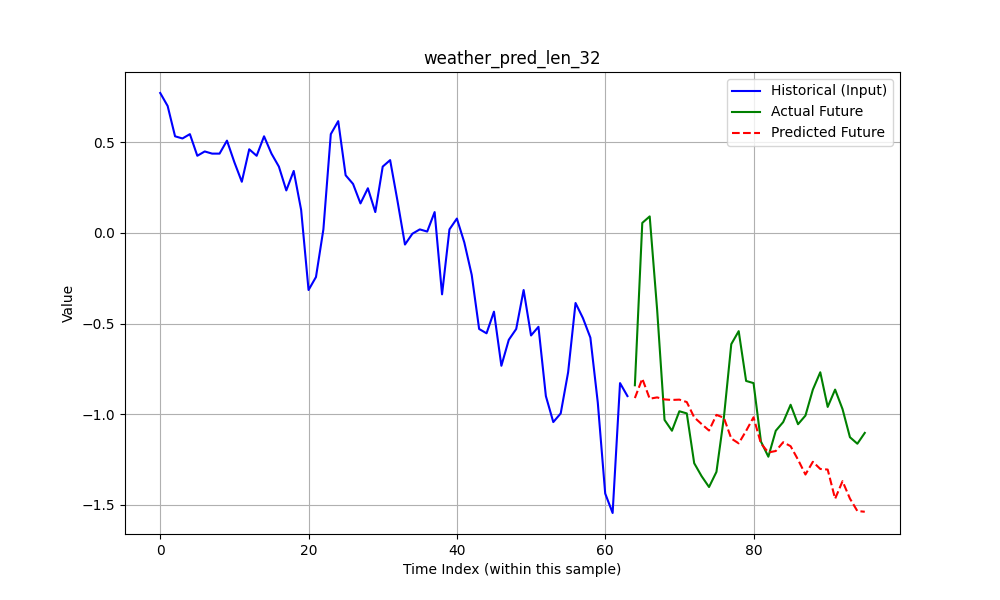
\includegraphics[width=\textwidth]{figures/samformer/weather_pred_len_32_sample_-1.png}
         \caption{Weather - Horizon 32}
    \end{subfigure}
    \begin{subfigure}[b]{0.32\textwidth}
         \centering
         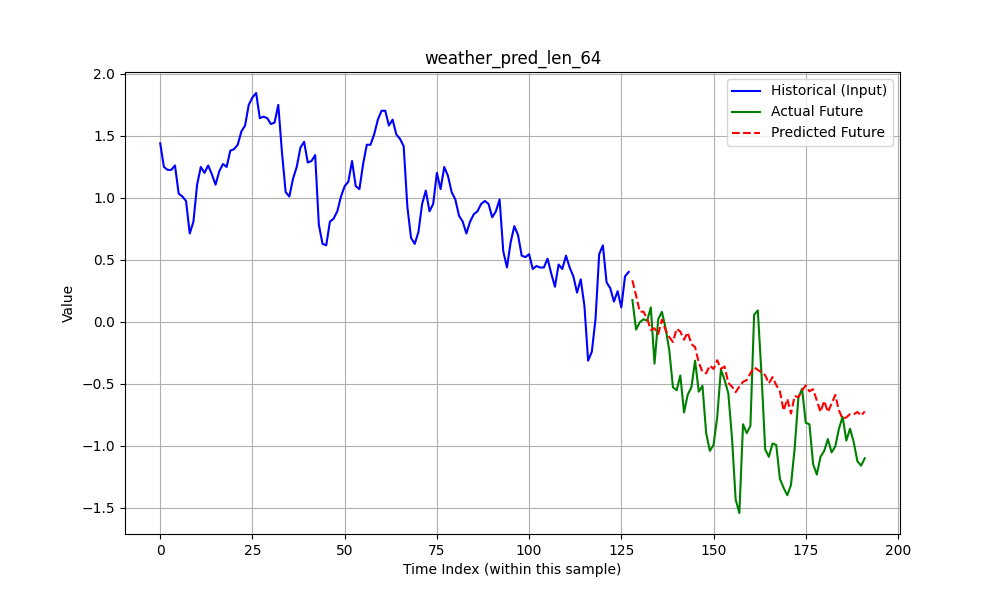
\includegraphics[width=\textwidth]{figures/samformer/weather_pred_len_64_sample_-1.png}
         \caption{Weather - Horizon 64}
    \end{subfigure}
    \begin{subfigure}[b]{0.32\textwidth}
         \centering
         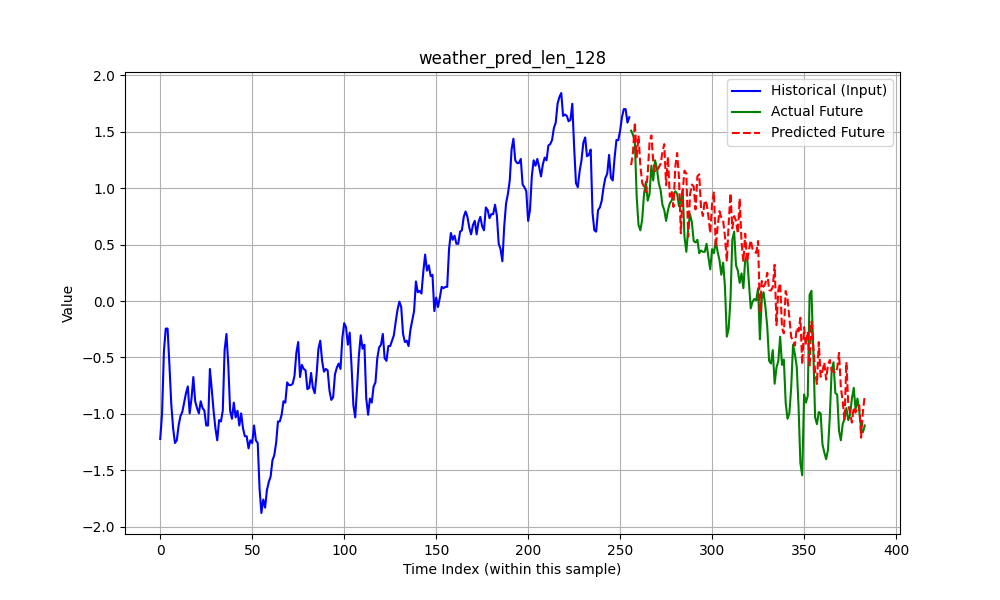
\includegraphics[width=\textwidth]{figures/samformer/weather_pred_len_128_sample_-1.png}
         \caption{Weather - Horizon 128}
    \end{subfigure}
    \caption{SAMFormer predictions on Weather dataset.}
\end{figure}

\begin{figure}[h!]
    \centering
    \begin{subfigure}[b]{0.32\textwidth}
         \centering
         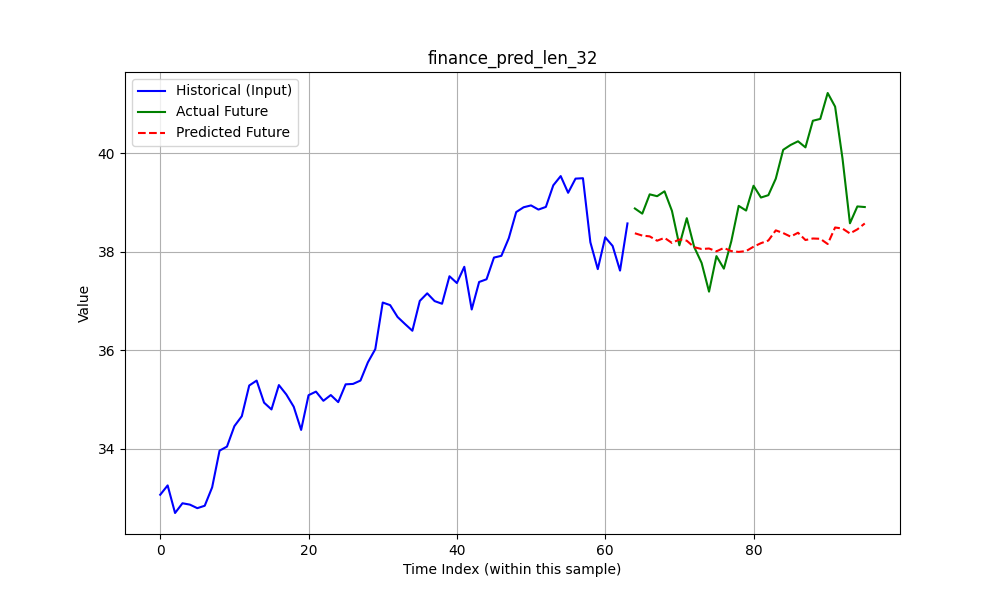
\includegraphics[width=\textwidth]{figures/samformer/finance_pred_len_32_sample_-1.png}
         \caption{Finance - Horizon 32}
    \end{subfigure}
    \begin{subfigure}[b]{0.32\textwidth}
         \centering
         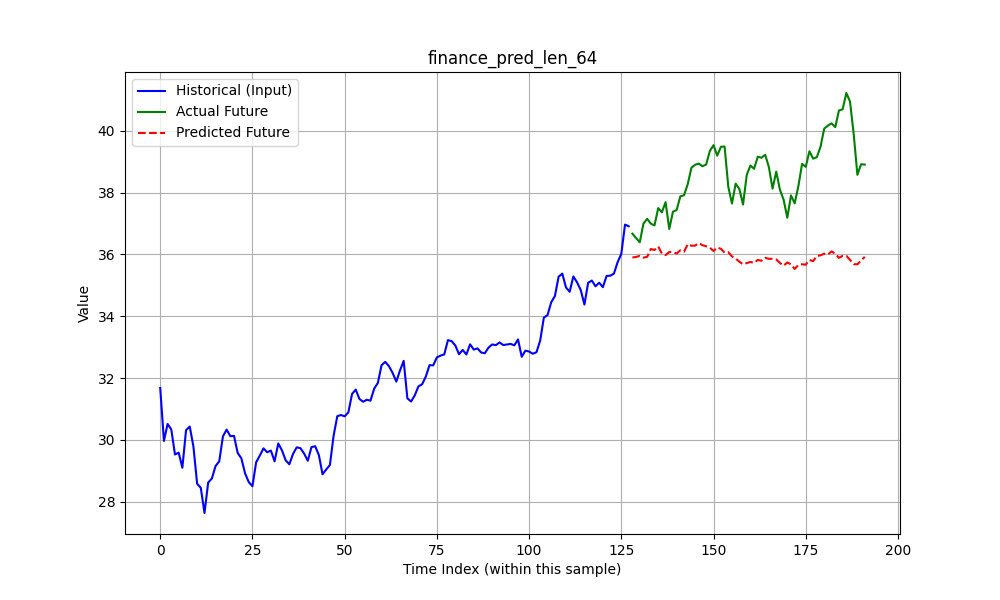
\includegraphics[width=\textwidth]{figures/samformer/finance_pred_len_64_sample_-1.png}
         \caption{Finance - Horizon 64}
    \end{subfigure}
    \begin{subfigure}[b]{0.32\textwidth}
         \centering
         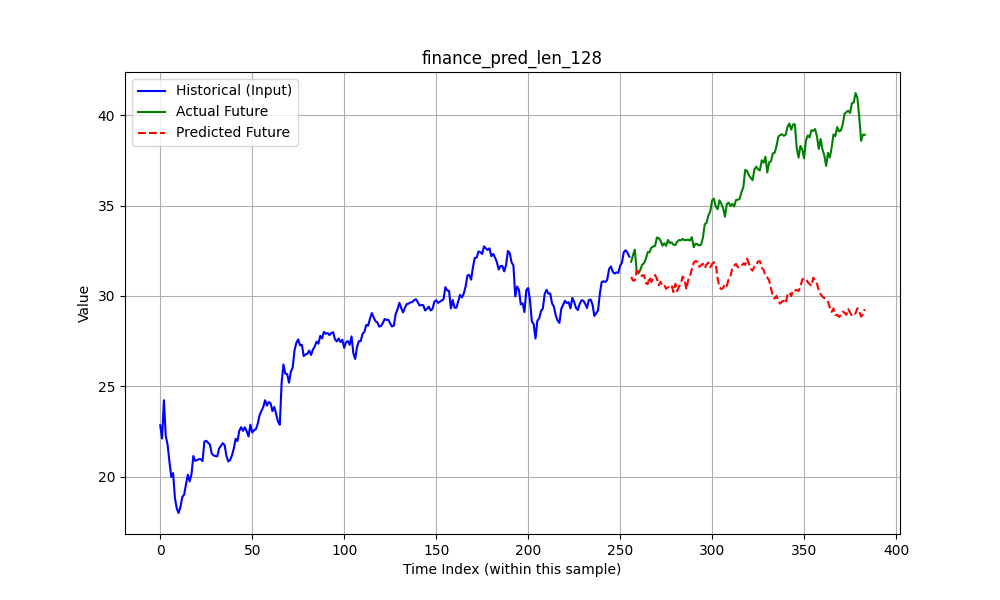
\includegraphics[width=\textwidth]{figures/samformer/finance_pred_len_128_sample_-1.png}
         \caption{Finance - Horizon 128}
    \end{subfigure}
    \caption{SAMFormer predictions on Finance dataset.}
\end{figure}

\begin{figure}[h!]
     \centering
     \begin{subfigure}[b]{0.32\textwidth}
          \centering
          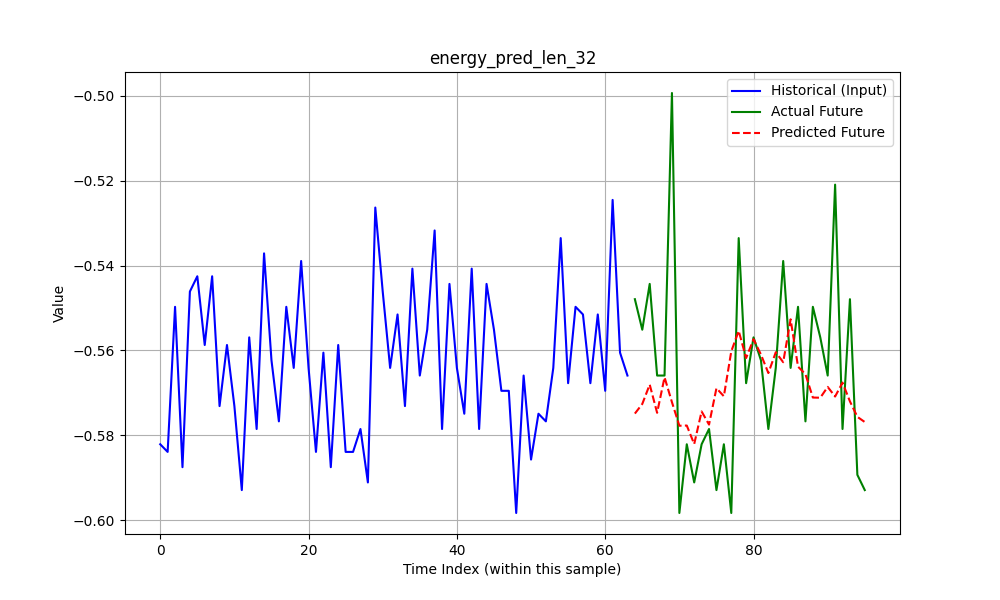
\includegraphics[width=\textwidth]{figures/samformer/energy_pred_len_32_sample_-1.png}
          \caption{Energy - Horizon 32}
     \end{subfigure}
     \begin{subfigure}[b]{0.32\textwidth}
          \centering
          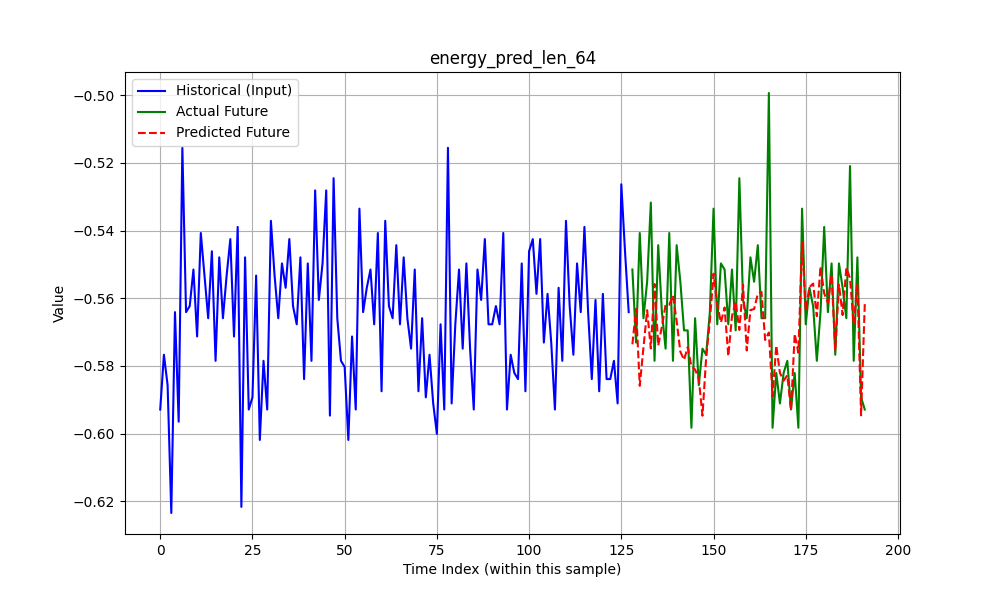
\includegraphics[width=\textwidth]{figures/samformer/energy_pred_len_64_sample_-1.png}
          \caption{Energy - Horizon 64}
     \end{subfigure}
     \begin{subfigure}[b]{0.32\textwidth}
          \centering
          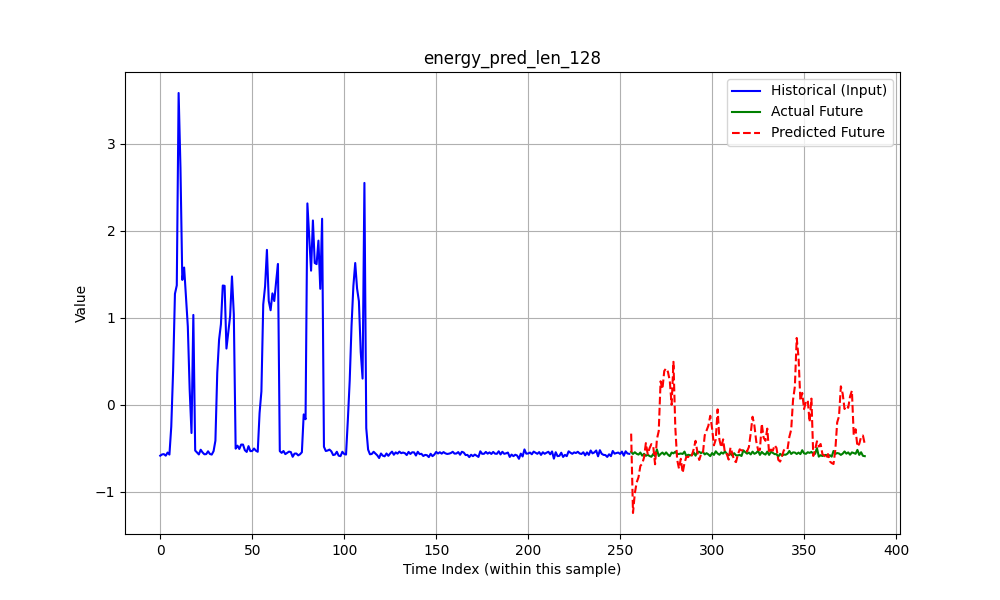
\includegraphics[width=\textwidth]{figures/samformer/energy_pred_len_128_sample_-1.png}
          \caption{Energy - Horizon 128}
     \end{subfigure}
     \caption{SAMFormer predictions on Healthcare dataset.}
 \end{figure}

 \begin{figure}[h!]
     \centering
     \begin{subfigure}[b]{0.32\textwidth}
          \centering
          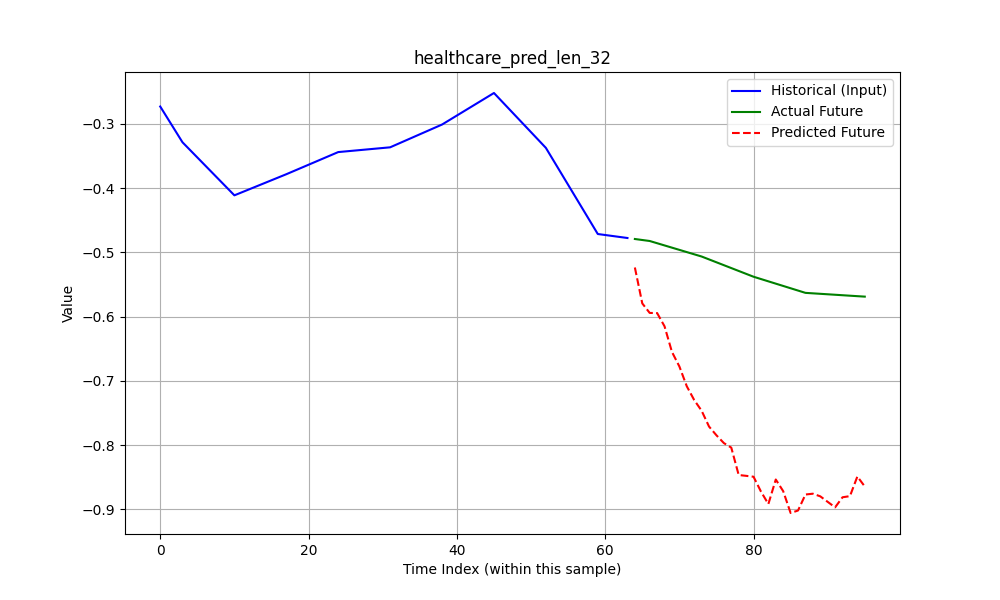
\includegraphics[width=\textwidth]{figures/samformer/healthcare_pred_len_32_sample_-1.png}
          \caption{Healthcare - Horizon 32}
     \end{subfigure}
     \begin{subfigure}[b]{0.32\textwidth}
          \centering
          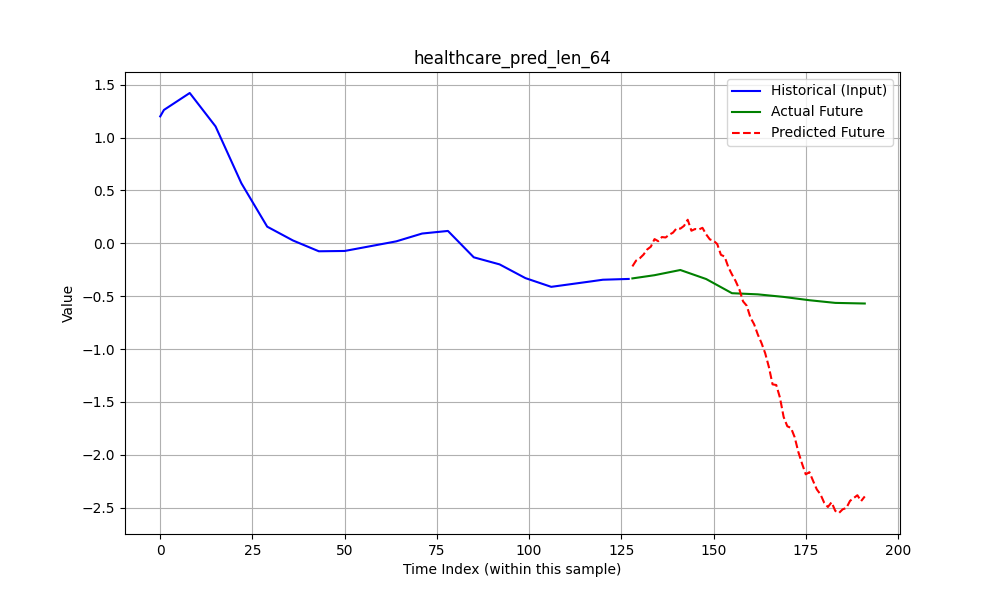
\includegraphics[width=\textwidth]{figures/samformer/healthcare_pred_len_64_sample_-1.png}
          \caption{Healthcare - Horizon 64}
     \end{subfigure}
     \begin{subfigure}[b]{0.32\textwidth}
          \centering
          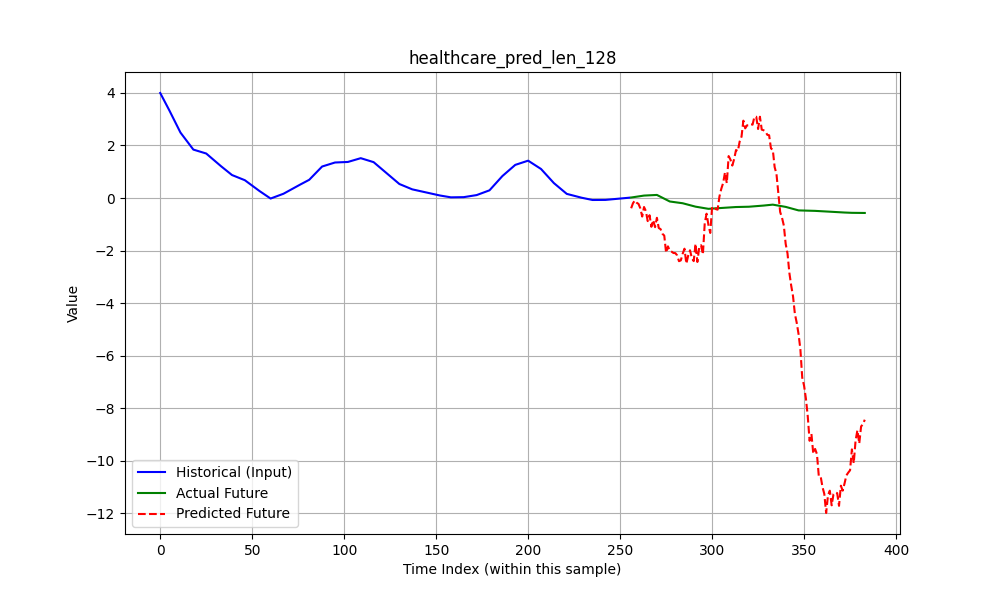
\includegraphics[width=\textwidth]{figures/samformer/healthcare_pred_len_128_sample_-1.png}
          \caption{Healthcare - Horizon 128}
     \end{subfigure}
     \caption{SAMFormer predictions on Healthcare dataset.}
 \end{figure}

\subsection{TimesFM}
\begin{figure}[h!]
    \centering
    \begin{subfigure}[b]{0.32\textwidth}
         \centering
         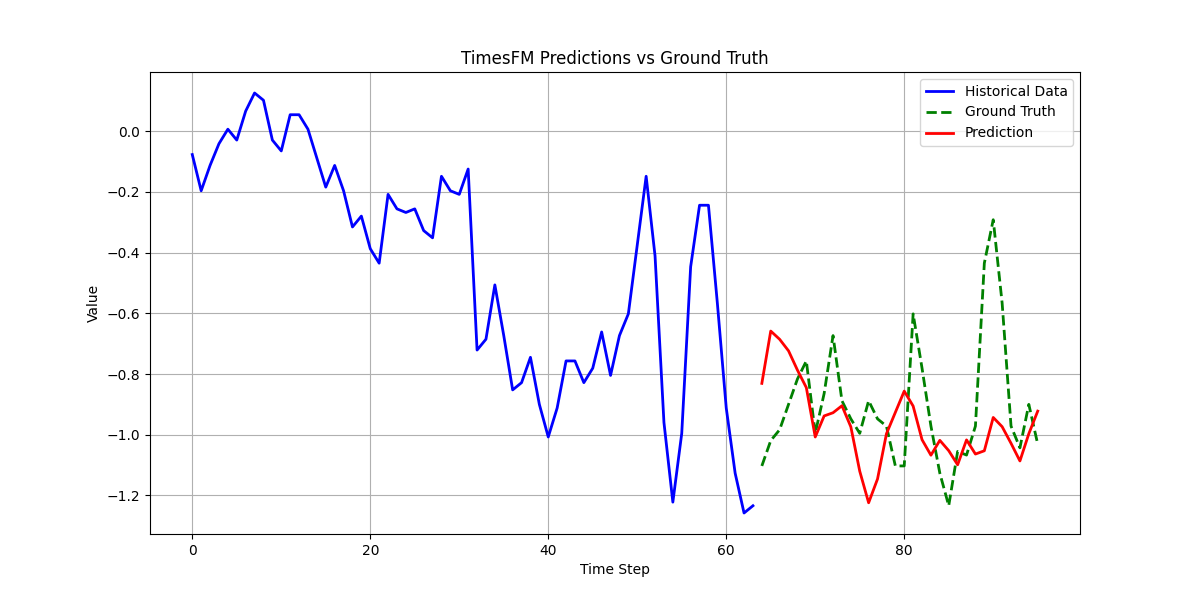
\includegraphics[width=\textwidth]{figures/timesfm/weather_predictions_exp1.png}
         \caption{Weather - Exp 1}
    \end{subfigure}
    \begin{subfigure}[b]{0.32\textwidth}
         \centering
         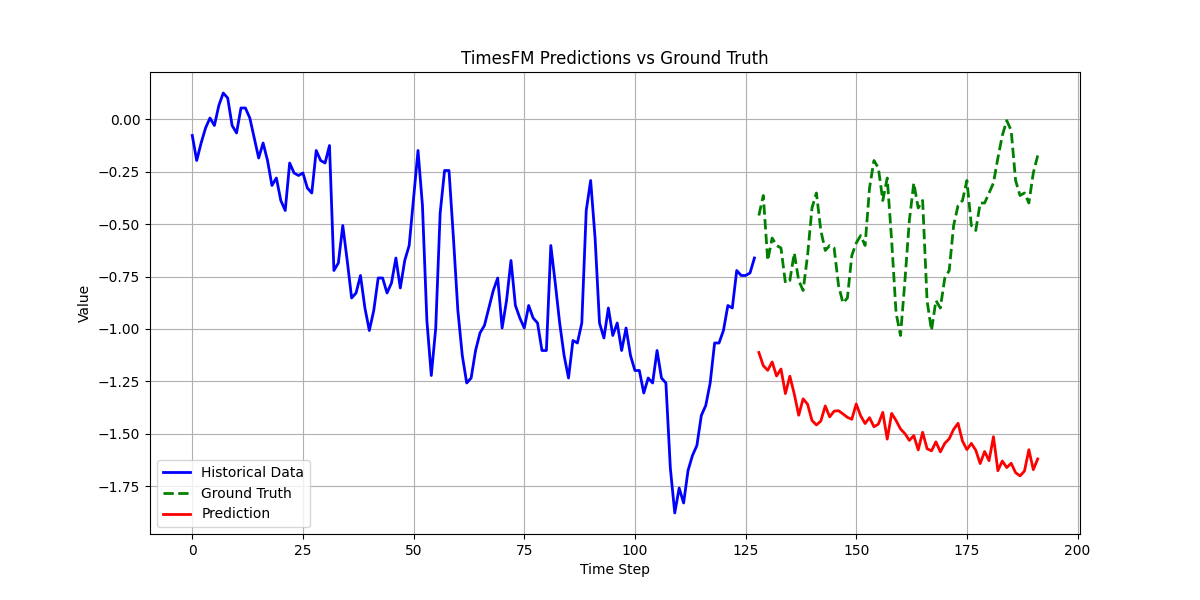
\includegraphics[width=\textwidth]{figures/timesfm/weather_predictions_exp2.png}
         \caption{Weather - Exp 2}
    \end{subfigure}
    \begin{subfigure}[b]{0.32\textwidth}
         \centering
         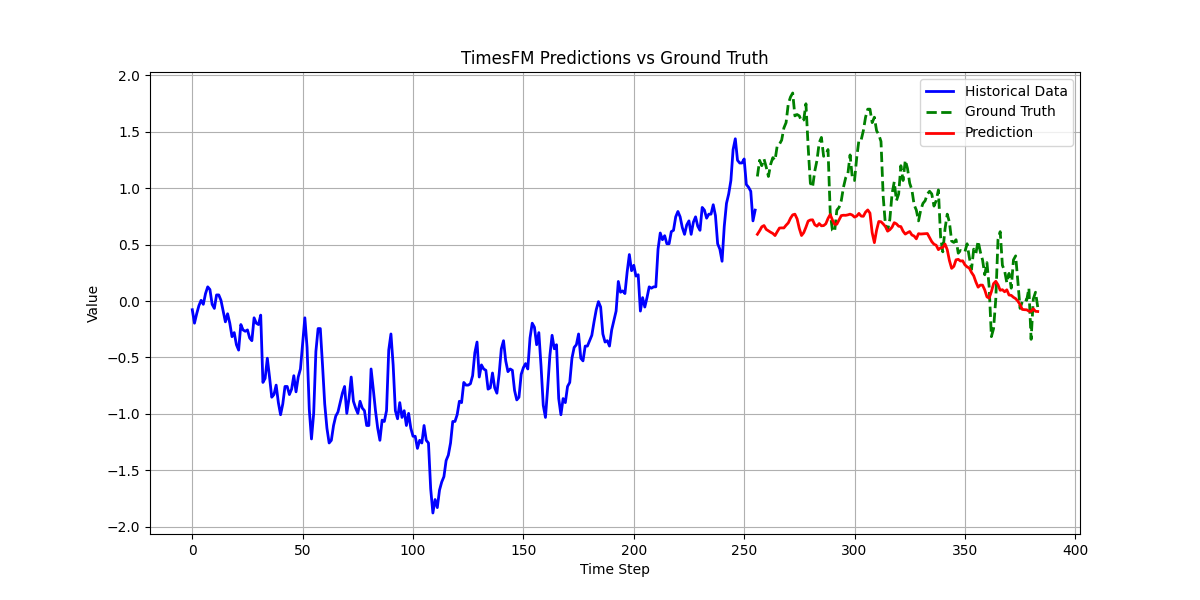
\includegraphics[width=\textwidth]{figures/timesfm/weather_predictions_exp3.png}
         \caption{Weather - Exp 3}
    \end{subfigure}
    \caption{TimesFM predictions on Weather dataset.}
\end{figure}

\begin{figure}[h!]
     \centering
     \begin{subfigure}[b]{0.32\textwidth}
          \centering
          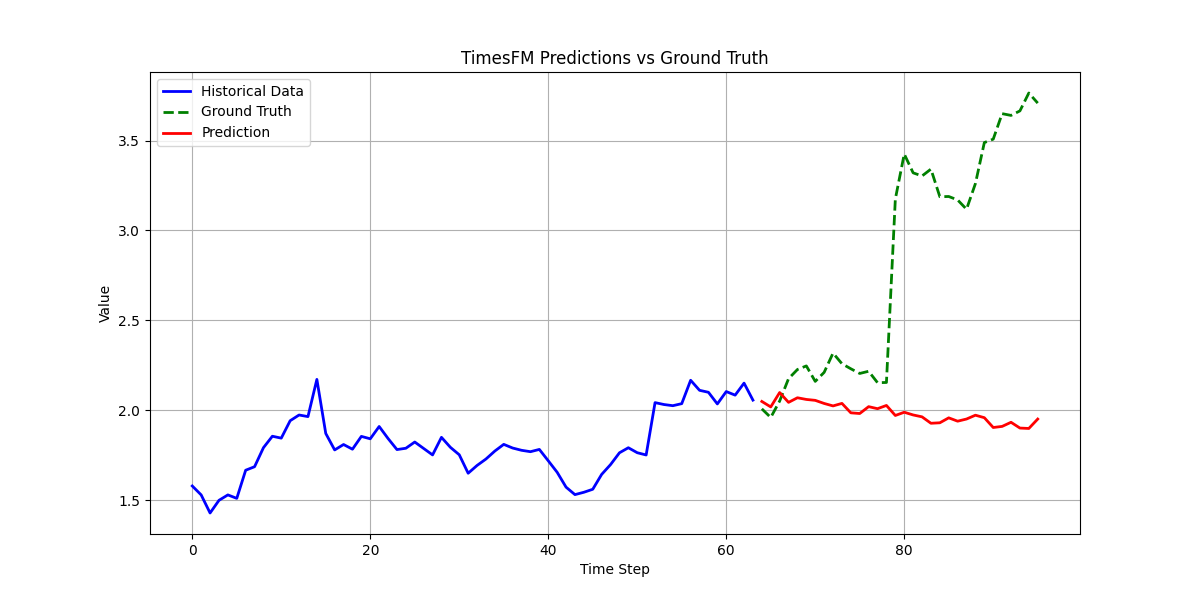
\includegraphics[width=\textwidth]{figures/timesfm/finance_predictions_exp1.png}
          \caption{Finance - Exp 1}
     \end{subfigure}
     \begin{subfigure}[b]{0.32\textwidth}
          \centering
          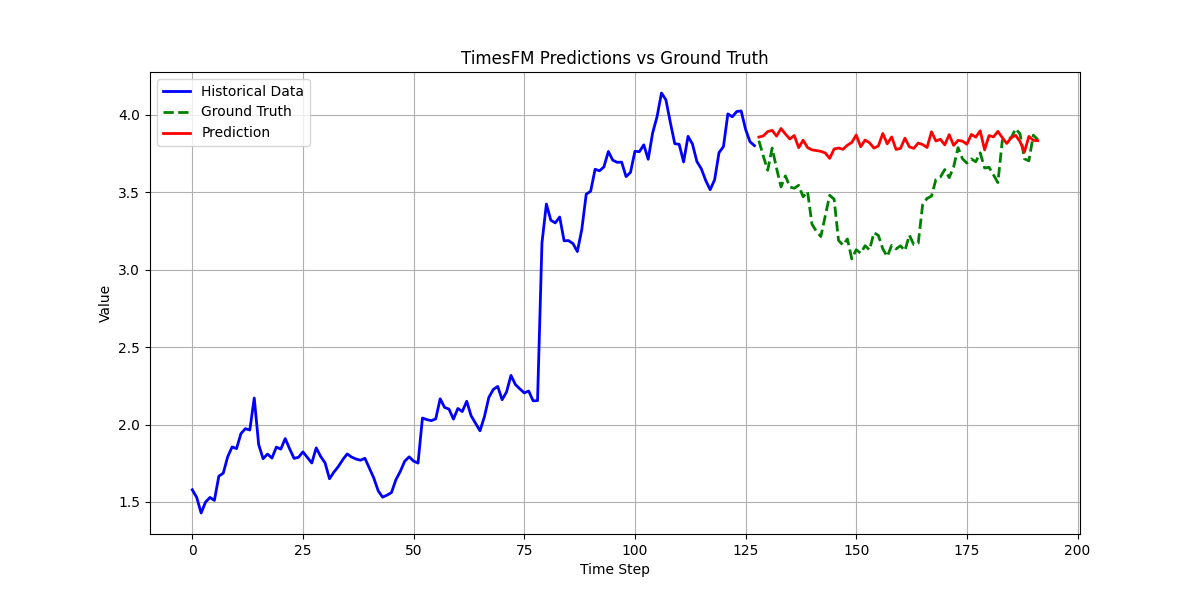
\includegraphics[width=\textwidth]{figures/timesfm/finance_predictions_exp2.png}
          \caption{Finance - Exp 2}
     \end{subfigure}
     \begin{subfigure}[b]{0.32\textwidth}
          \centering
          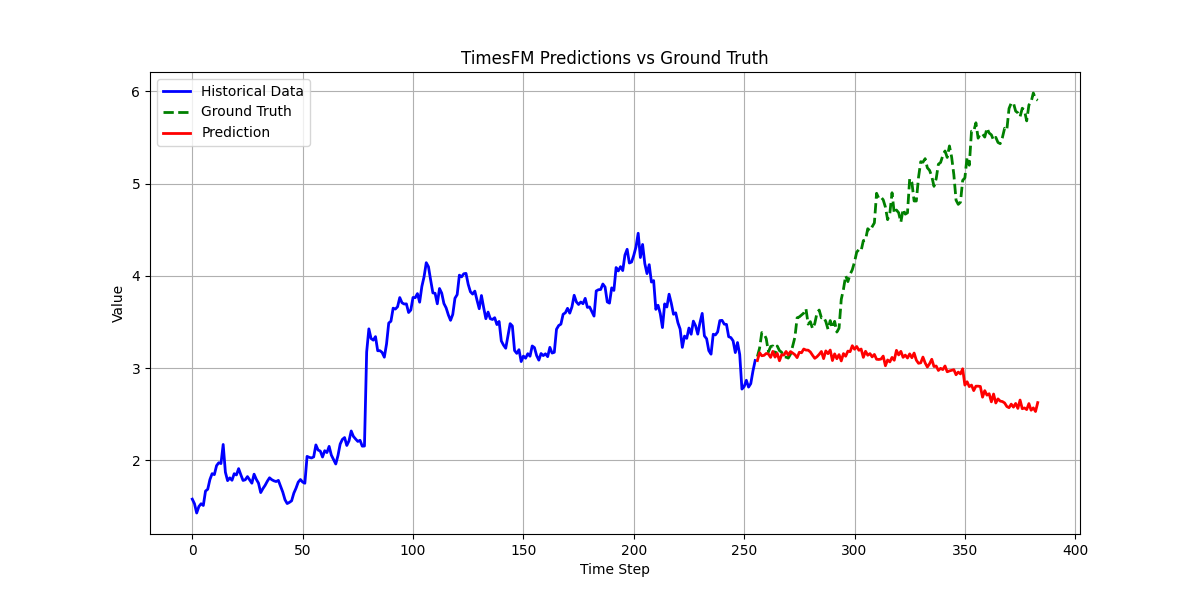
\includegraphics[width=\textwidth]{figures/timesfm/finance_predictions_exp3.png}
          \caption{Finance - Exp 3}
     \end{subfigure}
     \caption{TimesFM predictions on Finance dataset.}
 \end{figure}

 \begin{figure}[h!]
     \centering
     \begin{subfigure}[b]{0.32\textwidth}
          \centering
          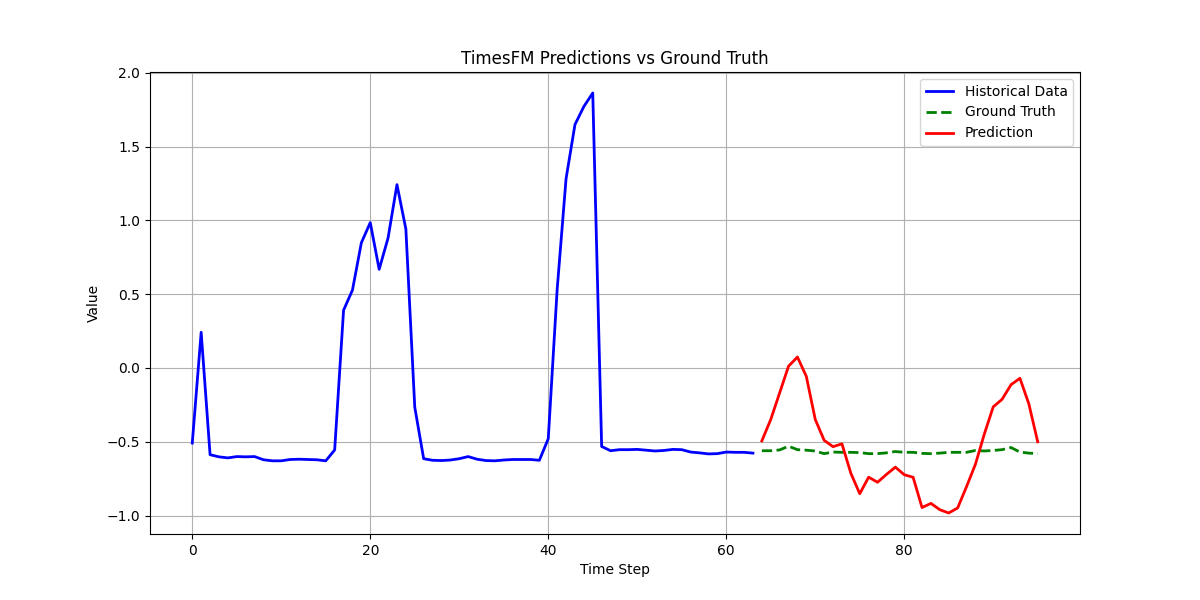
\includegraphics[width=\textwidth]{figures/timesfm/energy_predictions_exp1.png}
          \caption{Energy - Exp 1}
     \end{subfigure}
     \begin{subfigure}[b]{0.32\textwidth}
          \centering
          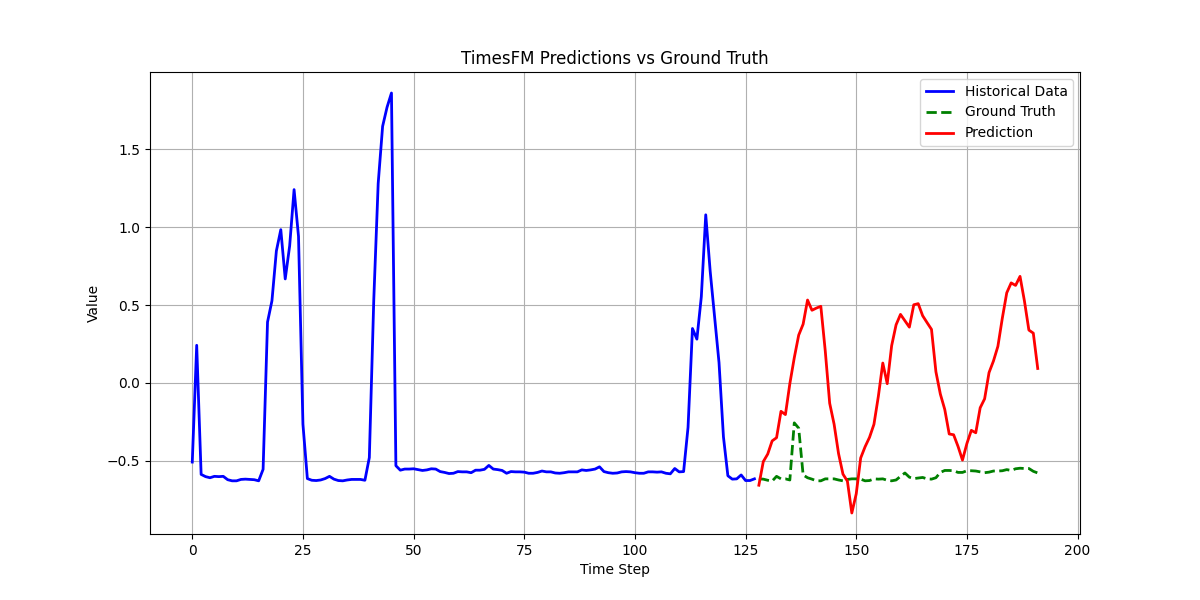
\includegraphics[width=\textwidth]{figures/timesfm/energy_predictions_exp2.png}
          \caption{Energy - Exp 2}
     \end{subfigure}
     \begin{subfigure}[b]{0.32\textwidth}
          \centering
          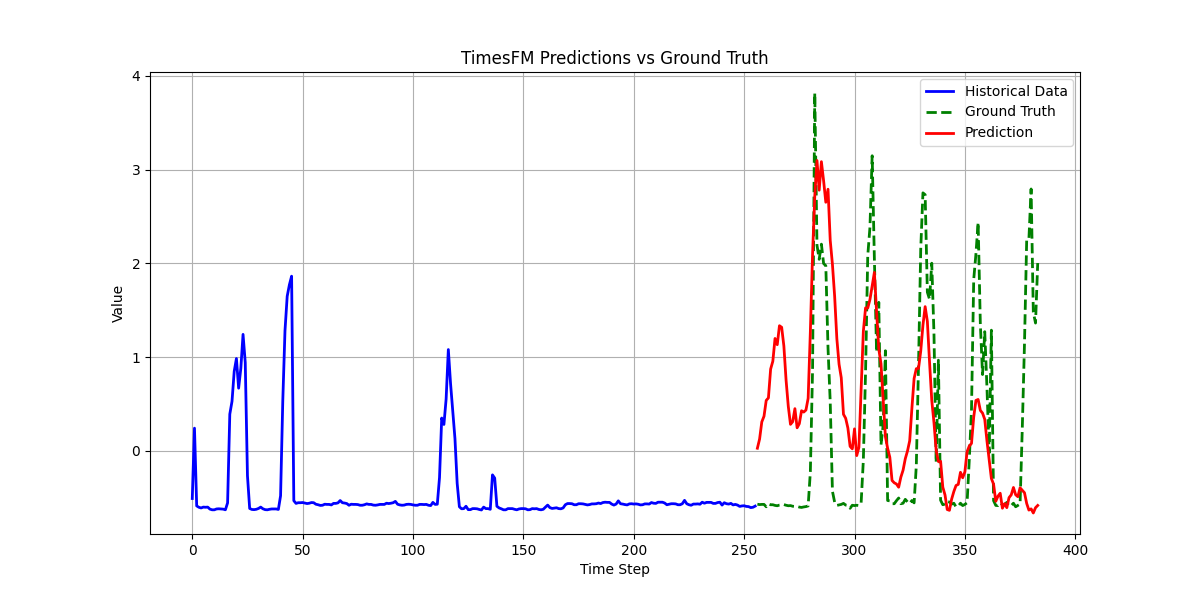
\includegraphics[width=\textwidth]{figures/timesfm/energy_predictions_exp3.png}
          \caption{Energy - Exp 3}
     \end{subfigure}
     \caption{TimesFM predictions on Energy dataset.}
 \end{figure}

 \begin{figure}[h!]
     \centering
     \begin{subfigure}[b]{0.32\textwidth}
          \centering
          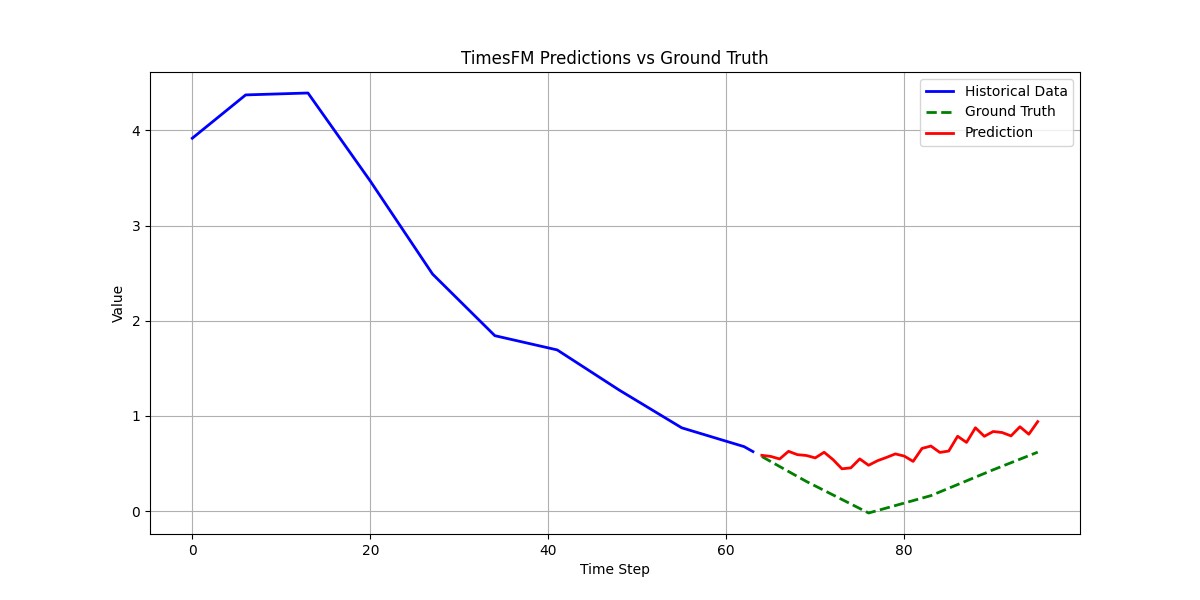
\includegraphics[width=\textwidth]{figures/timesfm/healthcare_predictions_exp1.png}
          \caption{Healthcare - Exp 1}
     \end{subfigure}
     \begin{subfigure}[b]{0.32\textwidth}
          \centering
          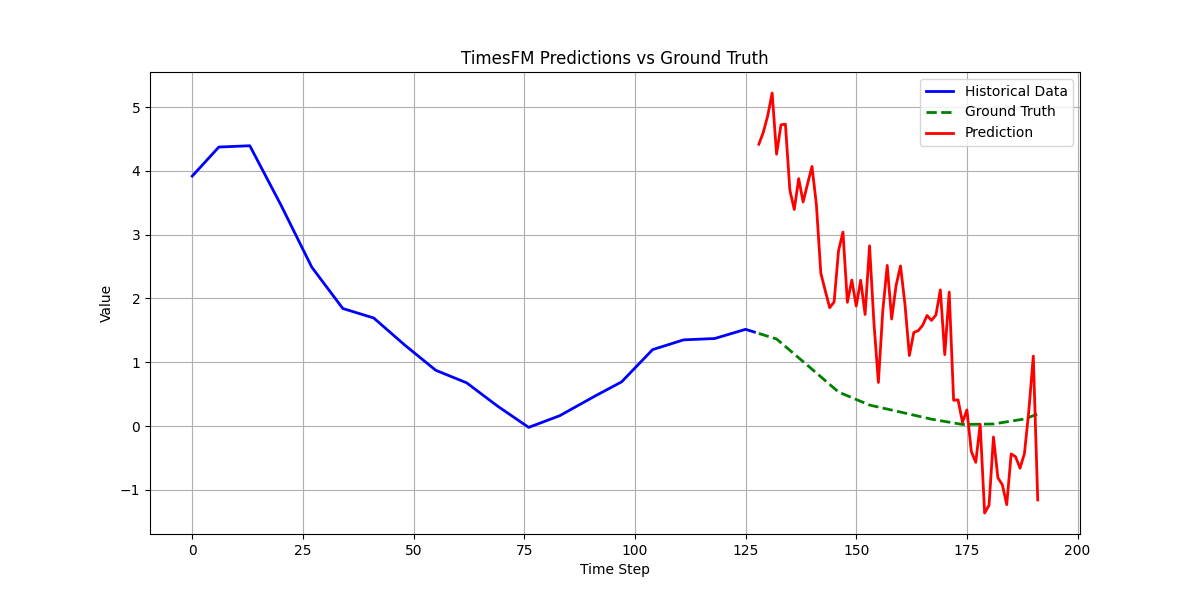
\includegraphics[width=\textwidth]{figures/timesfm/healthcare_predictions_exp2.png}
          \caption{Healthcare - Exp 2}
     \end{subfigure}
     \begin{subfigure}[b]{0.32\textwidth}
          \centering
          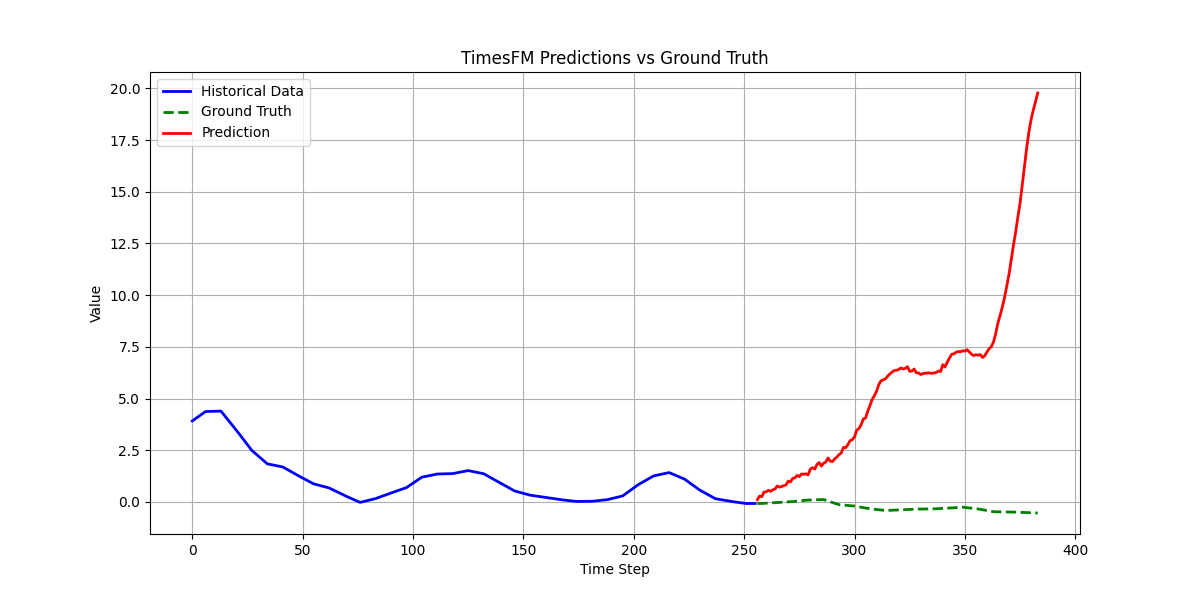
\includegraphics[width=\textwidth]{figures/timesfm/healthcare_predictions_exp3.png}
          \caption{Healhcare - Exp 3}
     \end{subfigure}
     \caption{TimesFM predictions on Healhcare dataset.}
 \end{figure}

\subsection{TimeGPT}
\begin{figure}[h!]
    \centering
    \begin{subfigure}[b]{0.32\textwidth}
         \centering
         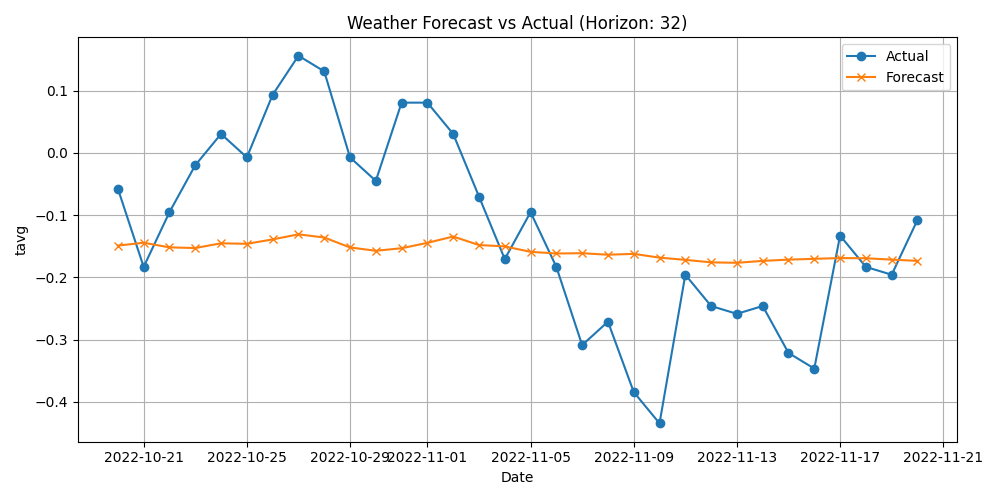
\includegraphics[width=\textwidth]{figures/timegpt/weather_32_forecast_plot.png}
         \caption{Weather - Horizon 32}
    \end{subfigure}
    \begin{subfigure}[b]{0.32\textwidth}
         \centering
         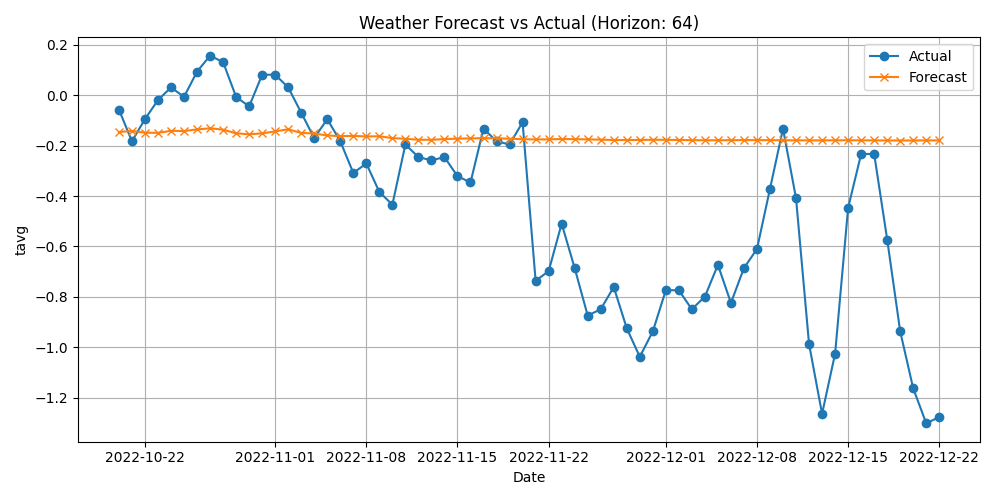
\includegraphics[width=\textwidth]{figures/timegpt/weather_64_forecast_plot.png}
         \caption{Weather - Horizon 64}
    \end{subfigure}
    \begin{subfigure}[b]{0.32\textwidth}
         \centering
         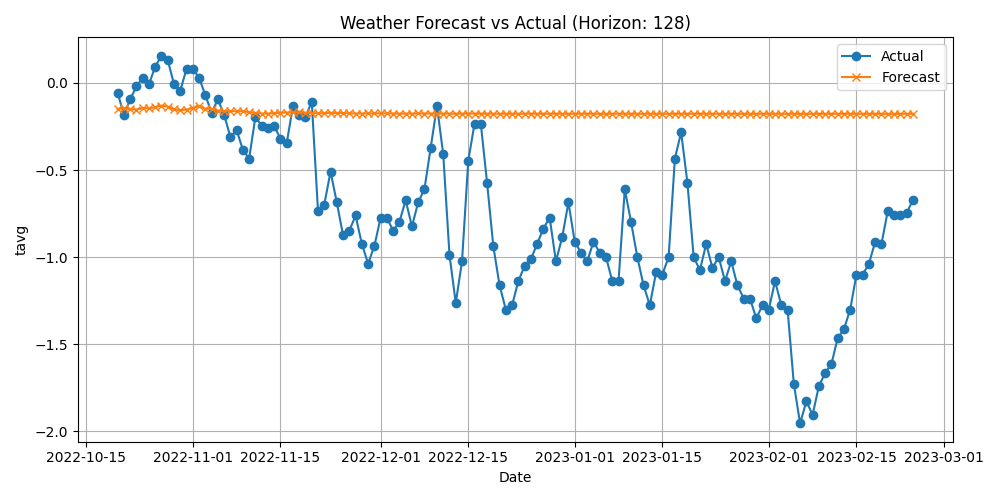
\includegraphics[width=\textwidth]{figures/timegpt/weather_128_forecast_plot.png}
         \caption{Weather - Horizon 128}
    \end{subfigure}
    \caption{TimeGPT predictions on Weather dataset.}
\end{figure}

\begin{figure}[h!]
     \centering
     \begin{subfigure}[b]{0.32\textwidth}
          \centering
          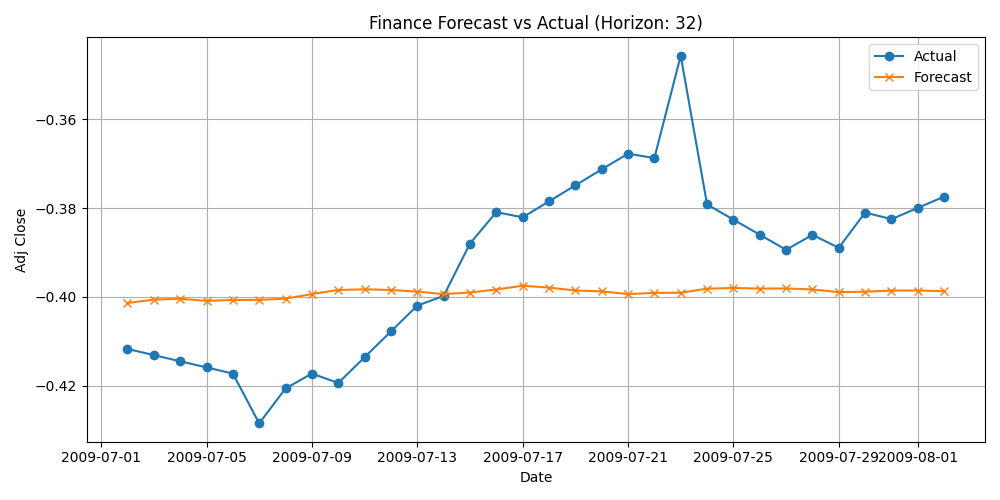
\includegraphics[width=\textwidth]{figures/timegpt/finance_32_forecast_plot.png}
          \caption{Finance - Horizon 32}
     \end{subfigure}
     \begin{subfigure}[b]{0.32\textwidth}
          \centering
          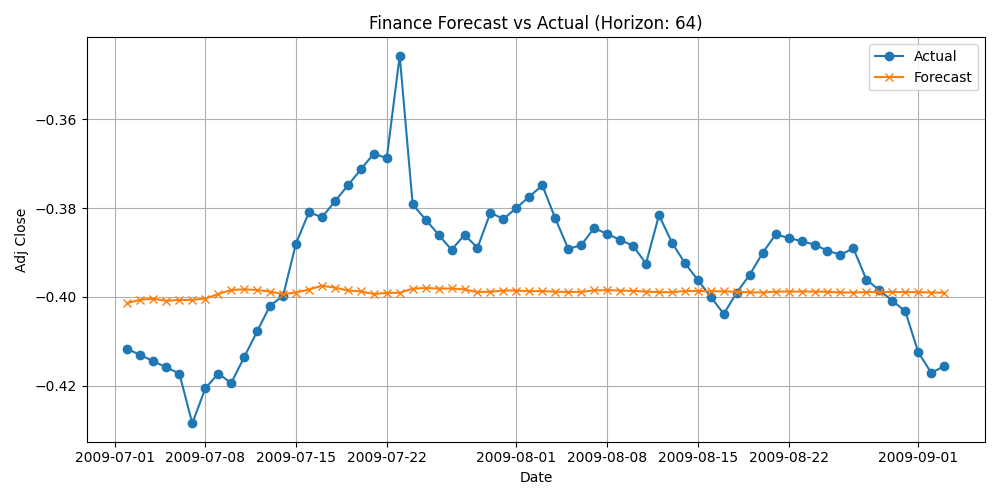
\includegraphics[width=\textwidth]{figures/timegpt/finance_64_forecast_plot.png}
          \caption{Finance - Horizon 64}
     \end{subfigure}
     \begin{subfigure}[b]{0.32\textwidth}
          \centering
          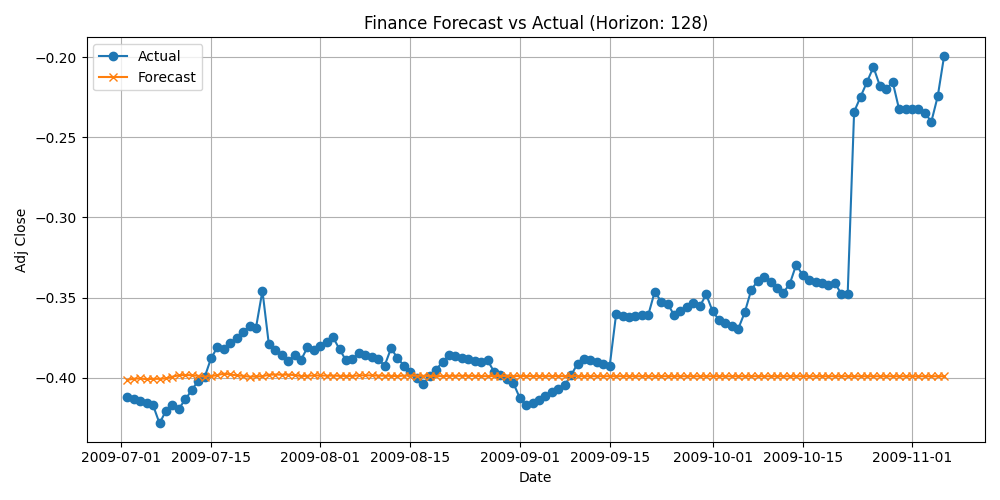
\includegraphics[width=\textwidth]{figures/timegpt/finance_128_forecast_plot.png}
          \caption{Finance - Horizon 128}
     \end{subfigure}
     \caption{TimeGPT predictions on Finance dataset.}
 \end{figure}

 \begin{figure}[h!]
     \centering
     \begin{subfigure}[b]{0.32\textwidth}
          \centering
          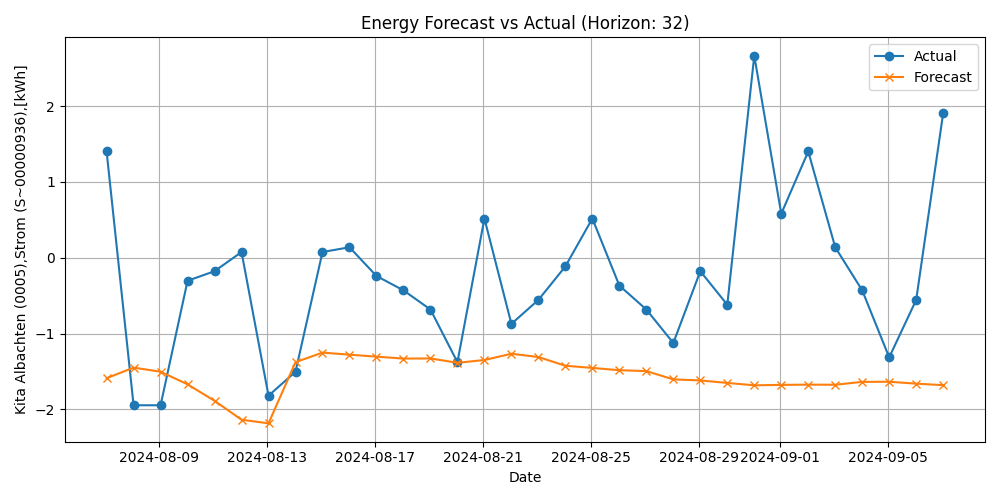
\includegraphics[width=\textwidth]{figures/timegpt/energy_32_forecast_plot.png}
          \caption{Energy - Horizon 32}
     \end{subfigure}
     \begin{subfigure}[b]{0.32\textwidth}
          \centering
          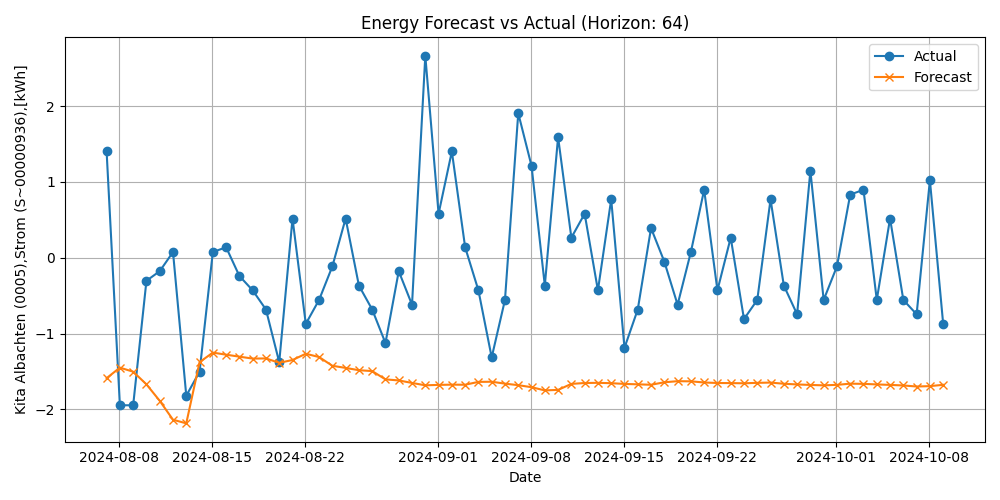
\includegraphics[width=\textwidth]{figures/timegpt/energy_64_forecast_plot.png}
          \caption{Energy - Horizon 64}
     \end{subfigure}
     \begin{subfigure}[b]{0.32\textwidth}
          \centering
          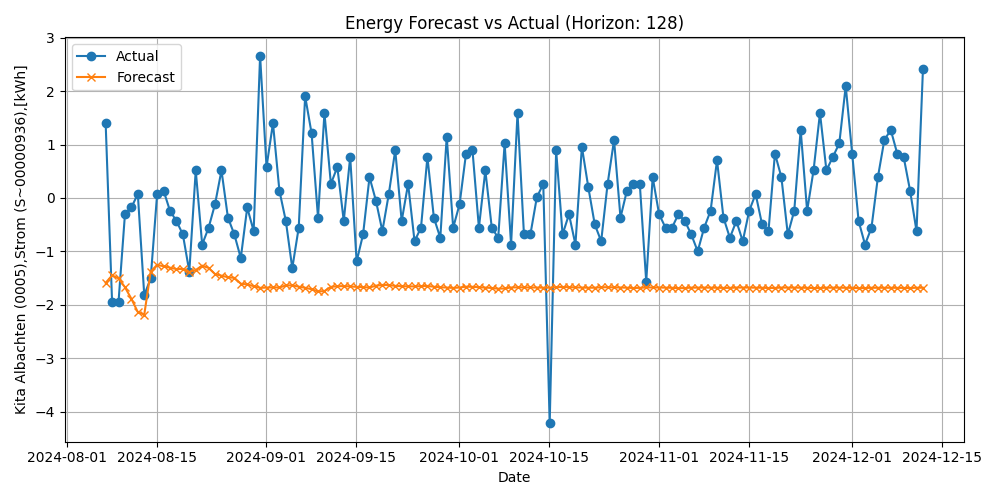
\includegraphics[width=\textwidth]{figures/timegpt/energy_128_forecast_plot.png}
          \caption{Energy - Horizon 128}
     \end{subfigure}
     \caption{TimeGPT predictions on Energy dataset.}
 \end{figure}

 \begin{figure}[h!]
     \centering
     \begin{subfigure}[b]{0.32\textwidth}
          \centering
          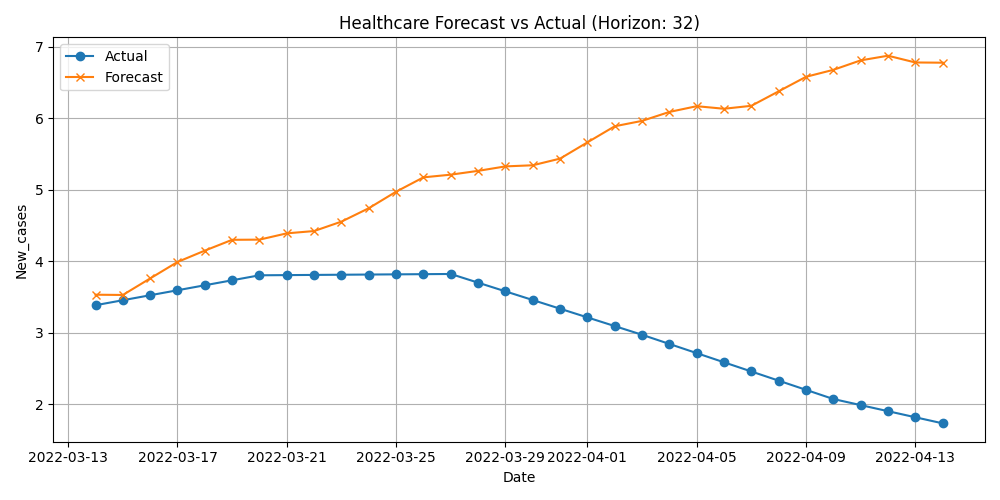
\includegraphics[width=\textwidth]{figures/timegpt/healthcare_32_forecast_plot.png}
          \caption{Healthcare - Horizon 32}
     \end{subfigure}
     \begin{subfigure}[b]{0.32\textwidth}
          \centering
          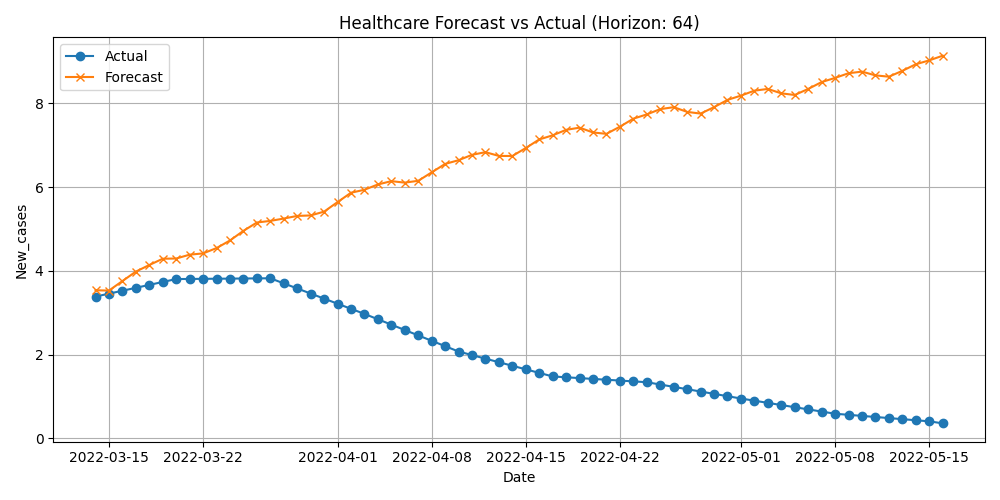
\includegraphics[width=\textwidth]{figures/timegpt/healthcare_64_forecast_plot.png}
          \caption{Healthcare - Horizon 64}
     \end{subfigure}
     \begin{subfigure}[b]{0.32\textwidth}
          \centering
          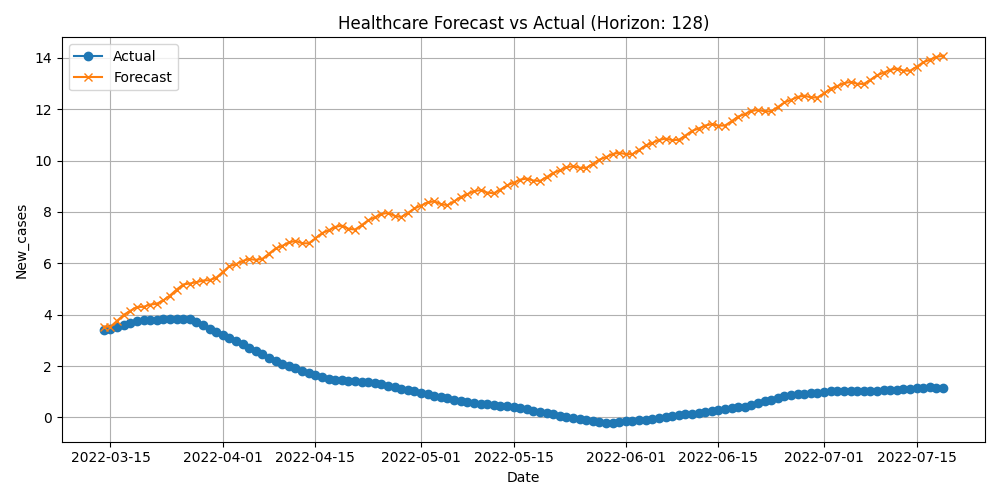
\includegraphics[width=\textwidth]{figures/timegpt/healthcare_128_forecast_plot.png}
          \caption{Healthcare - Horizon 128}
     \end{subfigure}
     \caption{TimeGPT predictions on Healthcare dataset.}
 \end{figure}

\subsection{Time-MoE}
\begin{figure}[h!]
    \centering
    \begin{subfigure}[b]{0.32\textwidth}
         \centering
         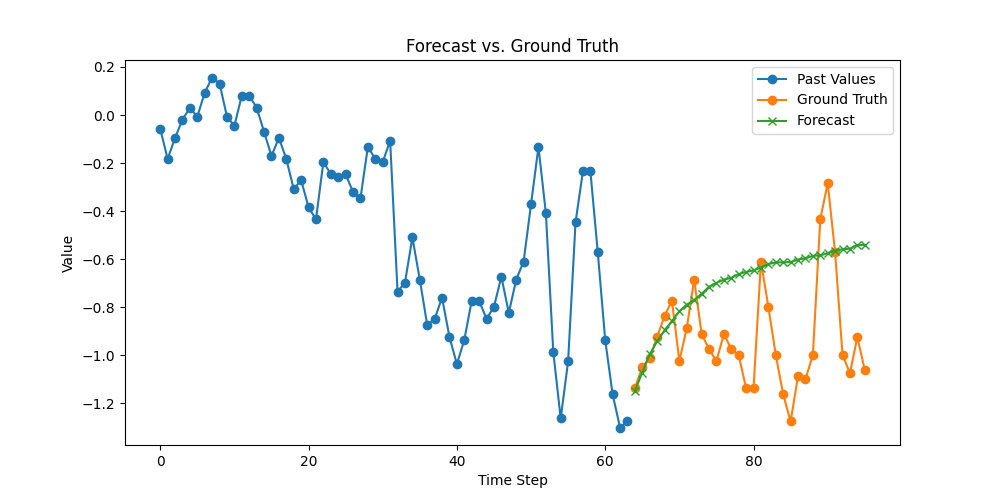
\includegraphics[width=\textwidth]{figures/time-moe/lezhe_64_32.png}
         \caption{Weather - Horizon 64$\to$32}
    \end{subfigure}
    \begin{subfigure}[b]{0.32\textwidth}
         \centering
         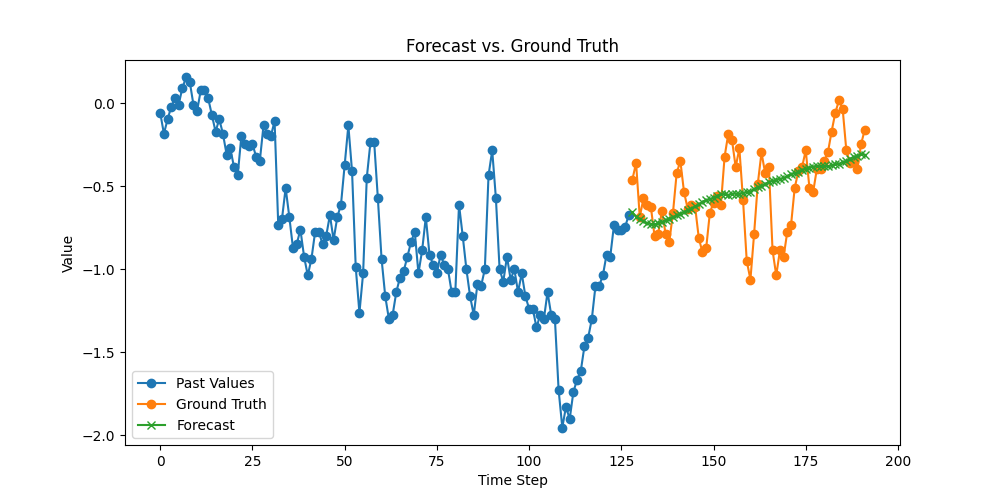
\includegraphics[width=\textwidth]{figures/time-moe/lezhe_128_64.png}
         \caption{Weather - Horizon 128$\to$64}
    \end{subfigure}
    \begin{subfigure}[b]{0.32\textwidth}
         \centering
         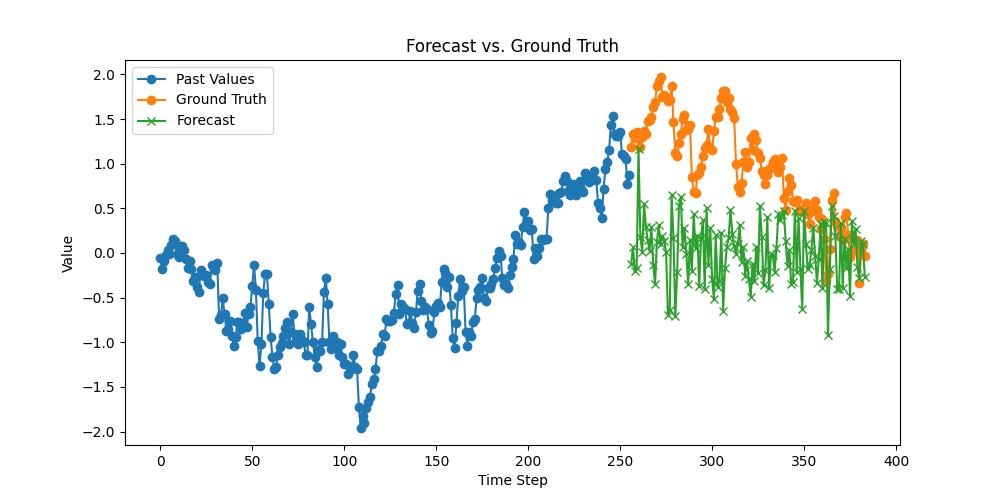
\includegraphics[width=\textwidth]{figures/time-moe/lezhe_256_128.png}
         \caption{Weather - Horizon 256$\to$128}
    \end{subfigure}
    \caption{Time-MoE predictions on Weather dataset.}
\end{figure}

\begin{figure}[h!]
     \centering
     \begin{subfigure}[b]{0.32\textwidth}
          \centering
          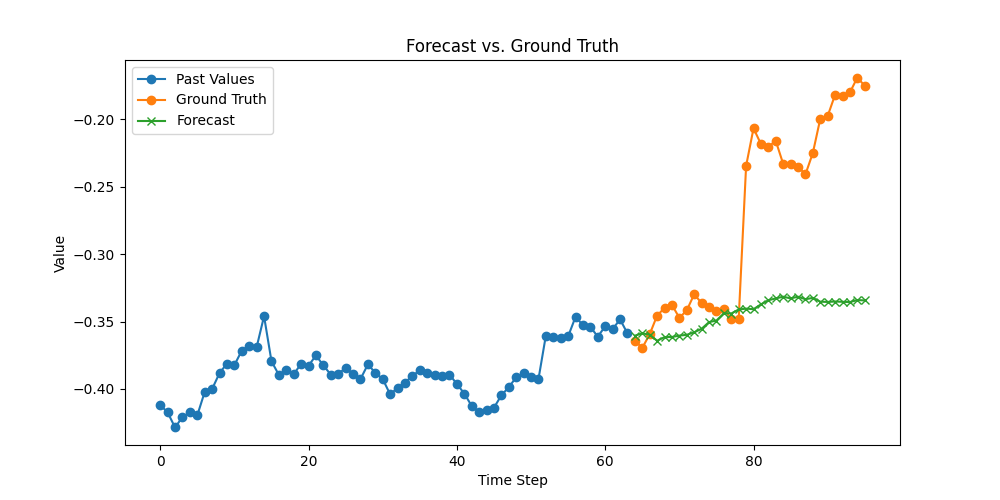
\includegraphics[width=\textwidth]{figures/time-moe/finance_64_32.png}
          \caption{Finance - Horizon 64$\to$32}
     \end{subfigure}
     \begin{subfigure}[b]{0.32\textwidth}
          \centering
          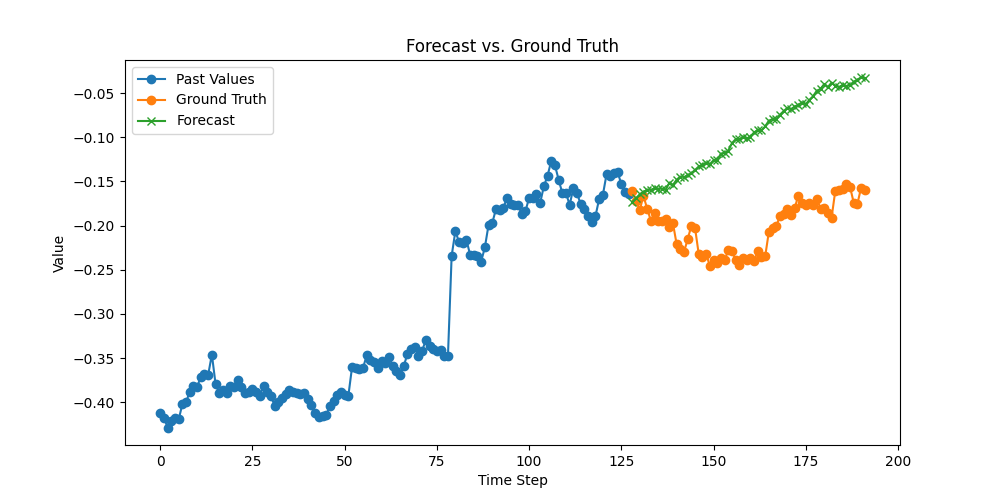
\includegraphics[width=\textwidth]{figures/time-moe/finance_128_64.png}
          \caption{Finance - Horizon 128$\to$64}
     \end{subfigure}
     \begin{subfigure}[b]{0.32\textwidth}
          \centering
          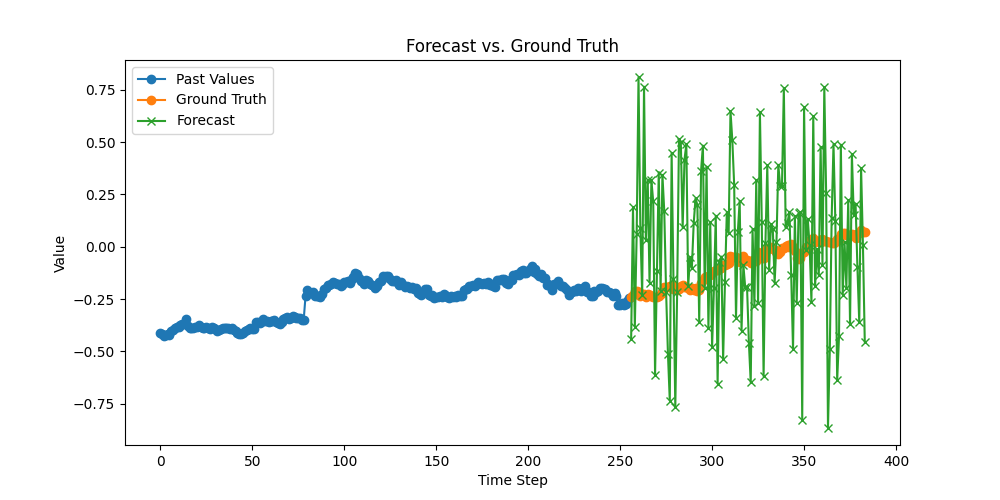
\includegraphics[width=\textwidth]{figures/time-moe/finance_256_128.png}
          \caption{Finance - Horizon 256$\to$128}
     \end{subfigure}
     \caption{Time-MoE predictions on Finance dataset.}
 \end{figure}

 \begin{figure}[h!]
     \centering
     \begin{subfigure}[b]{0.32\textwidth}
          \centering
          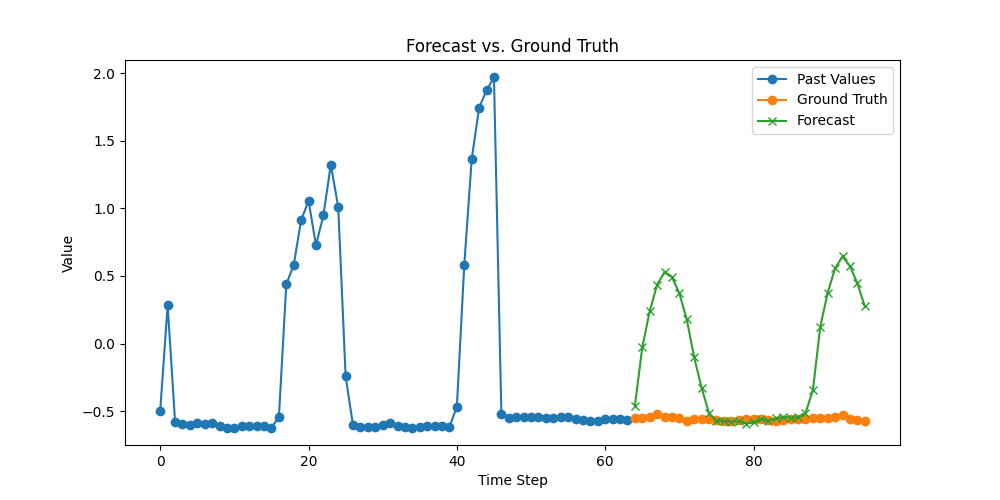
\includegraphics[width=\textwidth]{figures/time-moe/energy_64_32.png}
          \caption{Energy - Horizon 64$\to$32}
     \end{subfigure}
     \begin{subfigure}[b]{0.32\textwidth}
          \centering
          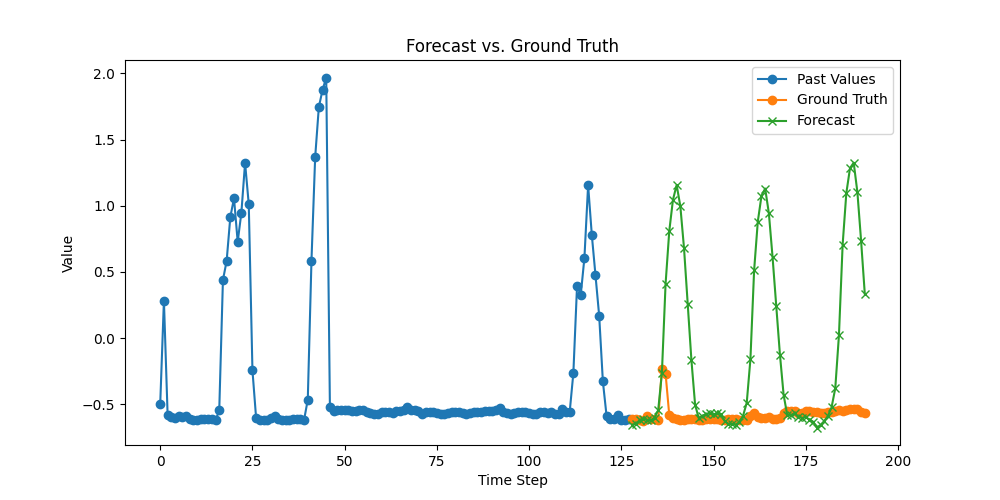
\includegraphics[width=\textwidth]{figures/time-moe/energy_128_64.png}
          \caption{Energy - Horizon 128$\to$64}
     \end{subfigure}
     \begin{subfigure}[b]{0.32\textwidth}
          \centering
          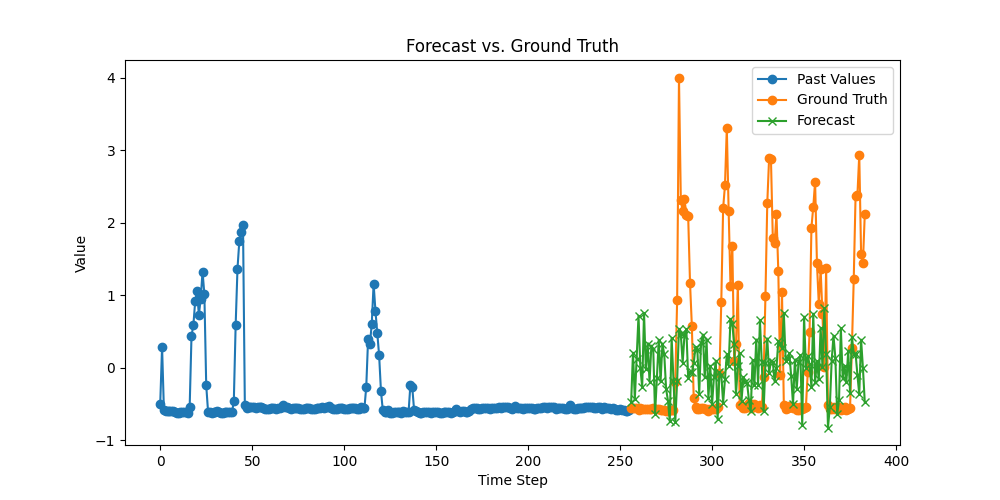
\includegraphics[width=\textwidth]{figures/time-moe/energy_256_128.png}
          \caption{Energy - Horizon 256$\to$128}
     \end{subfigure}
     \caption{Time-MoE predictions on Energy dataset.}
 \end{figure}

 \begin{figure}[h!]
     \centering
     \begin{subfigure}[b]{0.32\textwidth}
          \centering
          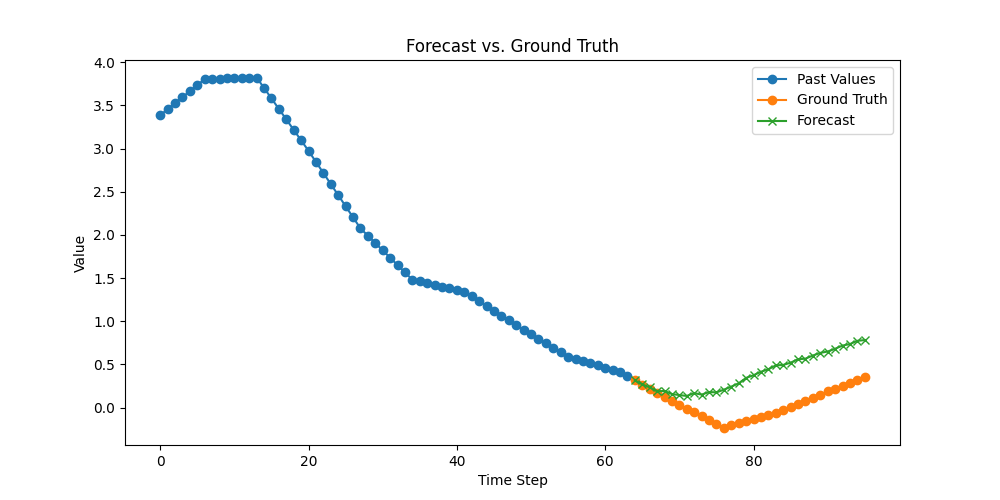
\includegraphics[width=\textwidth]{figures/time-moe/Germany_64_32.png}
          \caption{Healthcare - Horizon 64$\to$32}
     \end{subfigure}
     \begin{subfigure}[b]{0.32\textwidth}
          \centering
          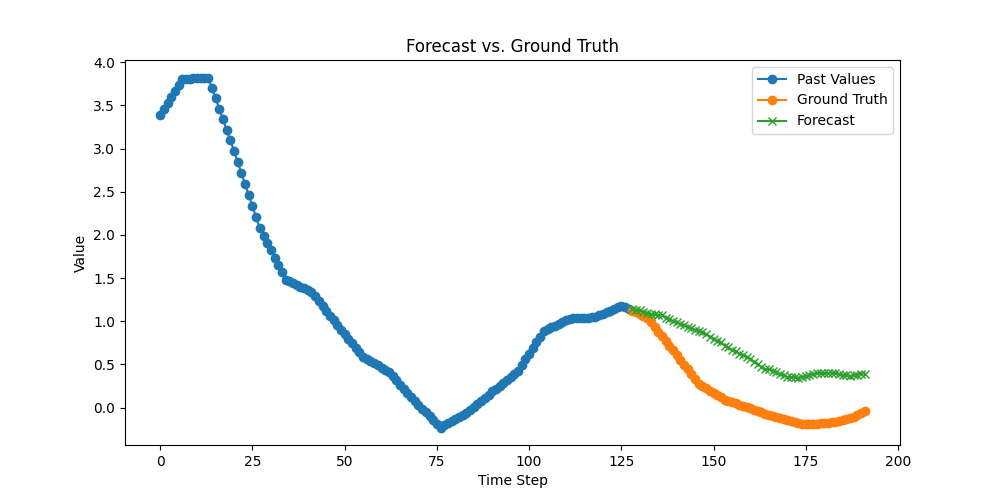
\includegraphics[width=\textwidth]{figures/time-moe/Germany_128_64.png}
          \caption{Healthcare - Horizon 128$\to$64}
     \end{subfigure}
     \begin{subfigure}[b]{0.32\textwidth}
          \centering
          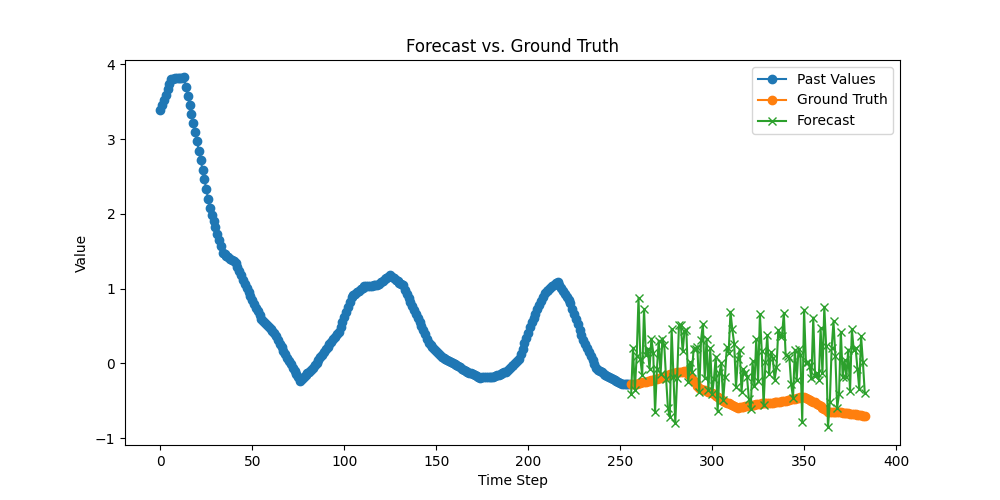
\includegraphics[width=\textwidth]{figures/time-moe/Germany_256_128.png}
          \caption{Healthcare - Horizon 256$\to$128}
     \end{subfigure}
     \caption{Time-MoE predictions on Healthcare dataset.}
 \end{figure}

\section{Regressors}

%---------------------------------------------------------
\subsection{Linear Regression}

\subsubsection{Weather Dataset}
\begin{figure}[h!]
    \centering
    \begin{subfigure}[b]{0.32\textwidth}
         \centering
         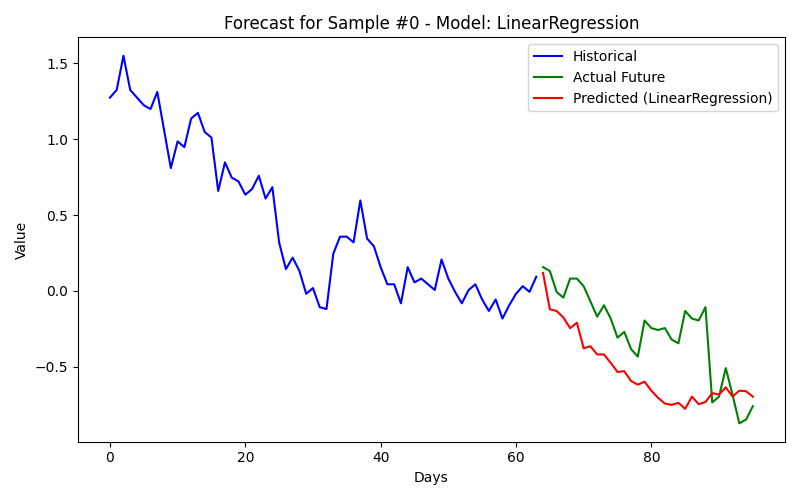
\includegraphics[width=\textwidth]{figures/regressors/LinearRegression/weather_64-32.png}
         \caption{Horizon 64$\to$32}
         \label{fig:LR_weather_64to32}
    \end{subfigure}
    \begin{subfigure}[b]{0.32\textwidth}
         \centering
         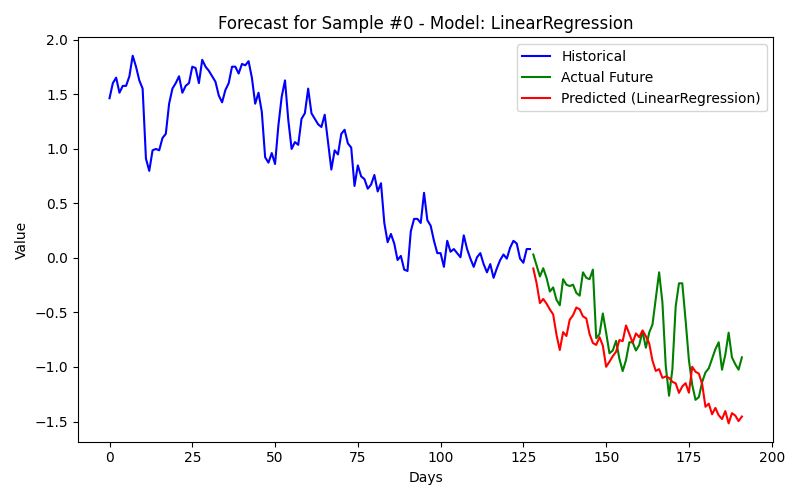
\includegraphics[width=\textwidth]{figures/regressors/LinearRegression/weather_128-64.png}
         \caption{Horizon 128$\to$64}
         \label{fig:LR_weather_128to64}
    \end{subfigure}
    \begin{subfigure}[b]{0.32\textwidth}
         \centering
         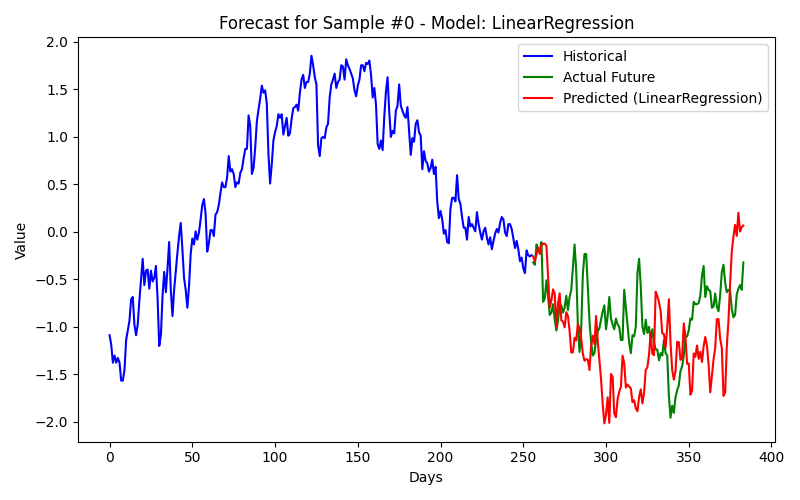
\includegraphics[width=\textwidth]{figures/regressors/LinearRegression/weather_256-128.png}
         \caption{Horizon 256$\to$128}
         \label{fig:LR_weather_256to128}
    \end{subfigure}
    \caption{Linear Regression forecasts on the Weather dataset for different horizons.}
    \label{fig:LR_weather_all}
\end{figure}

\subsubsection{Finance Dataset}
\begin{figure}[h!]
    \centering
    \begin{subfigure}[b]{0.32\textwidth}
         \centering
         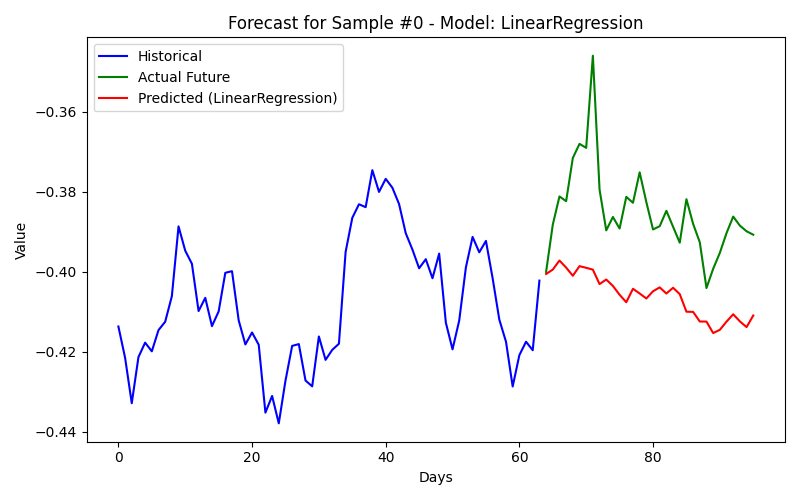
\includegraphics[width=\textwidth]{figures/regressors/LinearRegression/finance_64-32.png}
         \caption{Horizon 64$\to$32}
         \label{fig:LR_finance_64to32}
    \end{subfigure}
    \begin{subfigure}[b]{0.32\textwidth}
         \centering
         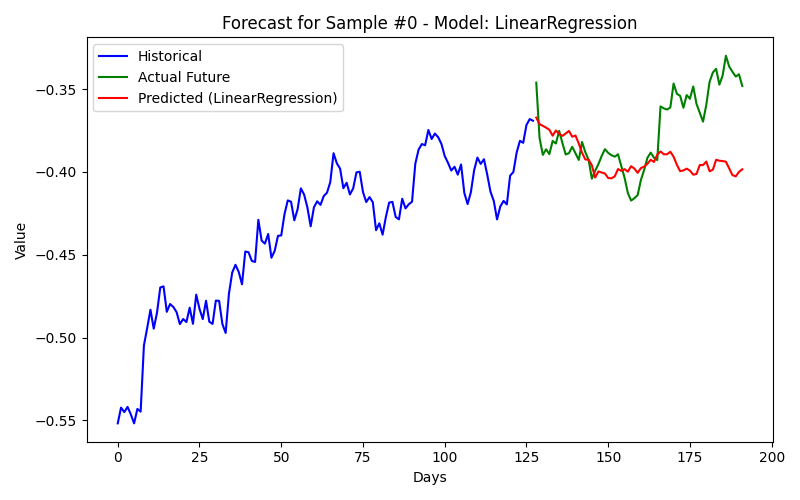
\includegraphics[width=\textwidth]{figures/regressors/LinearRegression/finance_128-64.png}
         \caption{Horizon 128$\to$64}
         \label{fig:LR_finance_128to64}
    \end{subfigure}
    \begin{subfigure}[b]{0.32\textwidth}
         \centering
         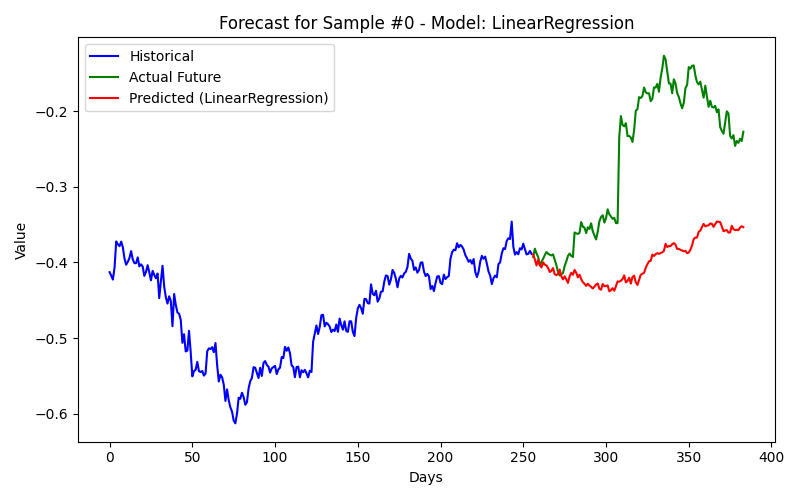
\includegraphics[width=\textwidth]{figures/regressors/LinearRegression/finance_256-128.png}
         \caption{Horizon 256$\to$128}
         \label{fig:LR_finance_256to128}
    \end{subfigure}
    \caption{Linear Regression forecasts on the Finance dataset for different horizons.}
    \label{fig:LR_finance_all}
\end{figure}

\subsubsection{Energy Dataset}
\begin{figure}[h!]
    \centering
    \begin{subfigure}[b]{0.32\textwidth}
         \centering
         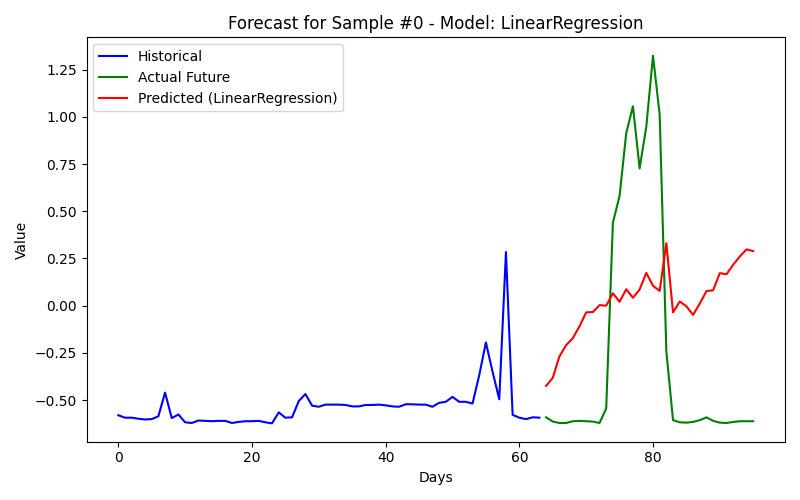
\includegraphics[width=\textwidth]{figures/regressors/LinearRegression/energy_64-32.png}
         \caption{Horizon 64$\to$32}
         \label{fig:LR_energy_64to32}
    \end{subfigure}
    \begin{subfigure}[b]{0.32\textwidth}
         \centering
         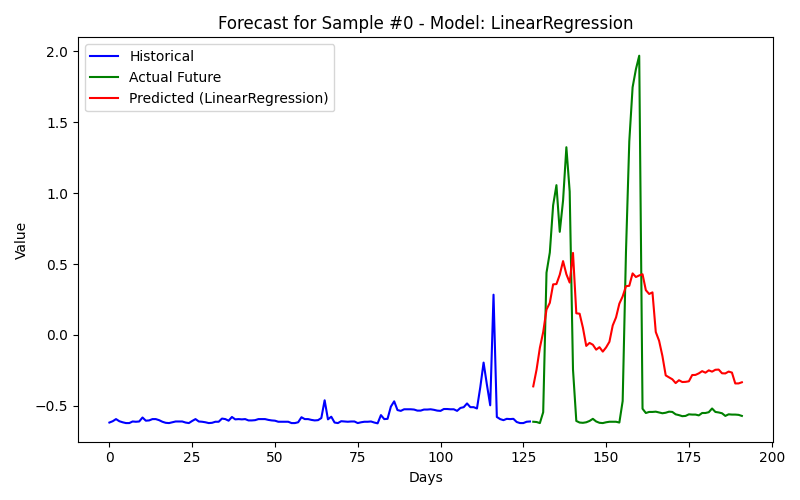
\includegraphics[width=\textwidth]{figures/regressors/LinearRegression/energy_128-64.png}
         \caption{Horizon 128$\to$64}
         \label{fig:LR_energy_128to64}
    \end{subfigure}
    \begin{subfigure}[b]{0.32\textwidth}
         \centering
         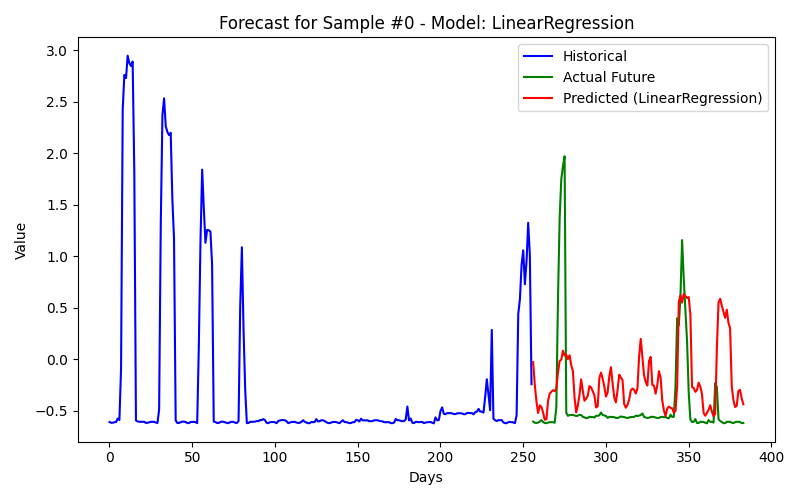
\includegraphics[width=\textwidth]{figures/regressors/LinearRegression/energy_256-128.png}
         \caption{Horizon 256$\to$128}
         \label{fig:LR_energy_256to128}
    \end{subfigure}
    \caption{Linear Regression forecasts on the Energy dataset for different horizons.}
    \label{fig:LR_energy_all}
\end{figure}

\subsubsection{Healthcare Dataset}
\begin{figure}[h!]
    \centering
    \begin{subfigure}[b]{0.32\textwidth}
         \centering
         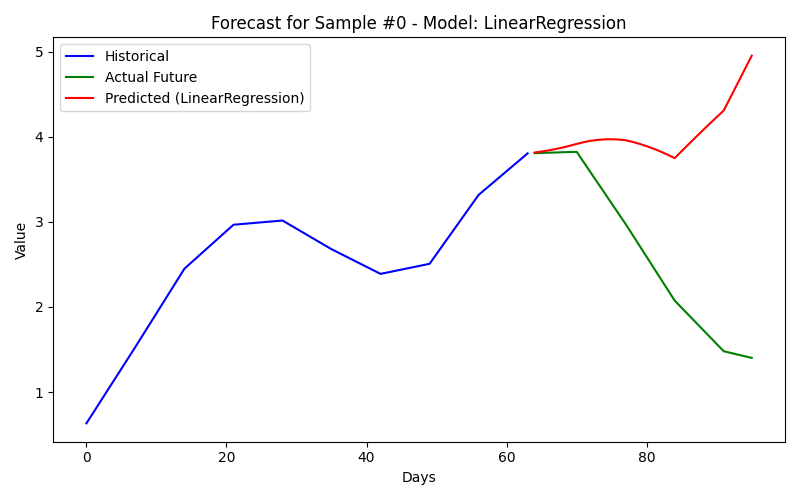
\includegraphics[width=\textwidth]{figures/regressors/LinearRegression/healthcare_64-32.png}
         \caption{Horizon 64$\to$32}
         \label{fig:LR_healthcare_64to32}
    \end{subfigure}
    \begin{subfigure}[b]{0.32\textwidth}
         \centering
         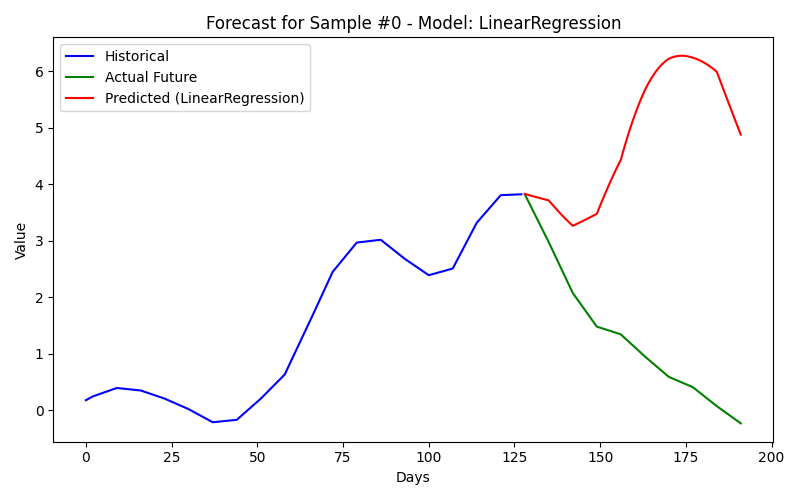
\includegraphics[width=\textwidth]{figures/regressors/LinearRegression/healthcare_128-64.png}
         \caption{Horizon 128$\to$64}
         \label{fig:LR_healthcare_128to64}
    \end{subfigure}
    \begin{subfigure}[b]{0.32\textwidth}
         \centering
         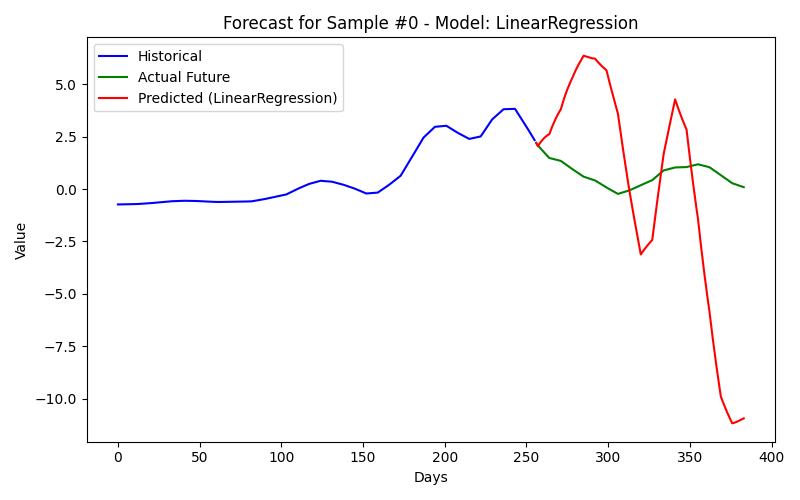
\includegraphics[width=\textwidth]{figures/regressors/LinearRegression/healthcare_256-128.png}
         \caption{Horizon 256$\to$128}
         \label{fig:LR_healthcare_256to128}
    \end{subfigure}
    \caption{Linear Regression forecasts on the Healthcare dataset for different horizons.}
    \label{fig:LR_healthcare_all}
\end{figure}

\newpage
%---------------------------------------------------------
\subsection{Random Forest Regressor}

\subsubsection{Weather Dataset}
\begin{figure}[h!]
    \centering
    \begin{subfigure}[b]{0.32\textwidth}
         \centering
         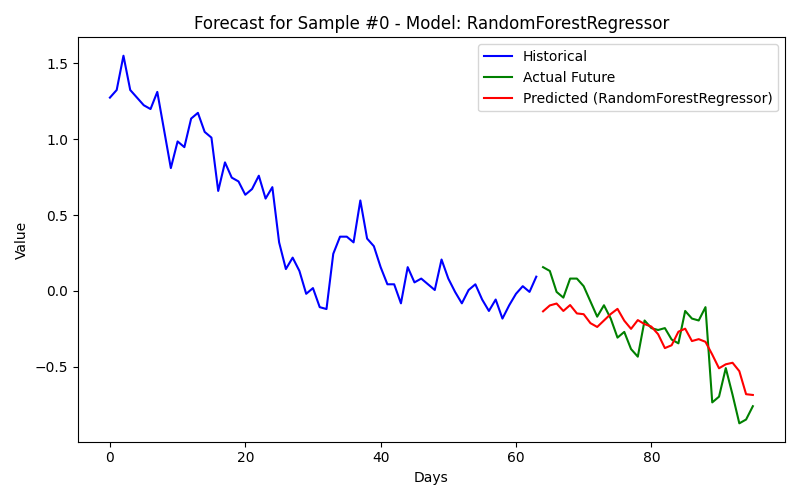
\includegraphics[width=\textwidth]{figures/regressors/RandomForestRegressor/weather_64-32.png}
         \caption{Horizon 64$\to$32}
         \label{fig:RF_weather_64to32}
    \end{subfigure}
    \begin{subfigure}[b]{0.32\textwidth}
         \centering
         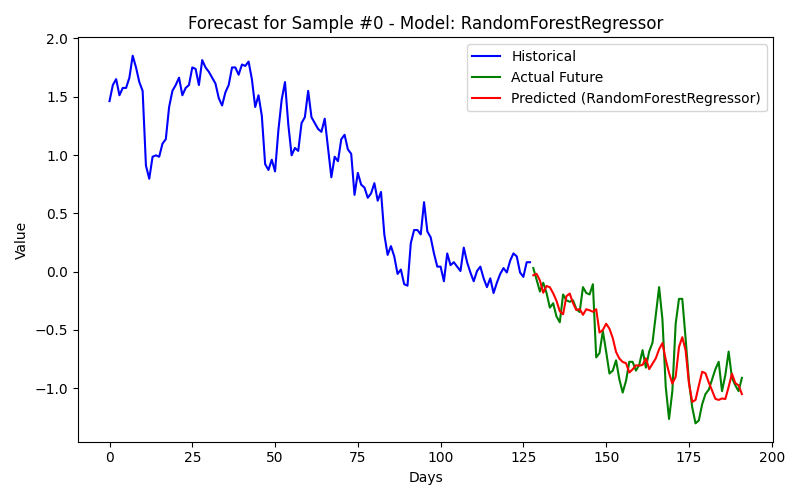
\includegraphics[width=\textwidth]{figures/regressors/RandomForestRegressor/weather_128-64.png}
         \caption{Horizon 128$\to$64}
         \label{fig:RF_weather_128to64}
    \end{subfigure}
    \begin{subfigure}[b]{0.32\textwidth}
         \centering
         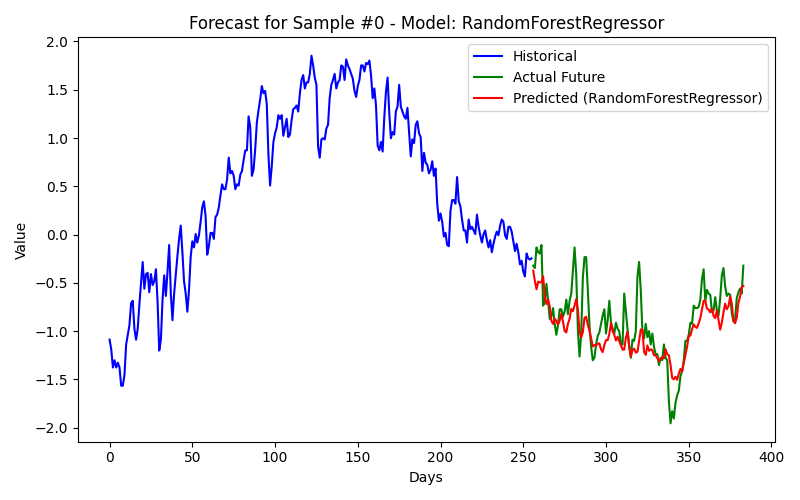
\includegraphics[width=\textwidth]{figures/regressors/RandomForestRegressor/weather_256-128.png}
         \caption{Horizon 256$\to$128}
         \label{fig:RF_weather_256to128}
    \end{subfigure}
    \caption{Random Forest forecasts on the Weather dataset for different horizons.}
    \label{fig:RF_weather_all}
\end{figure}

\subsubsection{Finance Dataset}
\begin{figure}[h!]
    \centering
    \begin{subfigure}[b]{0.32\textwidth}
         \centering
         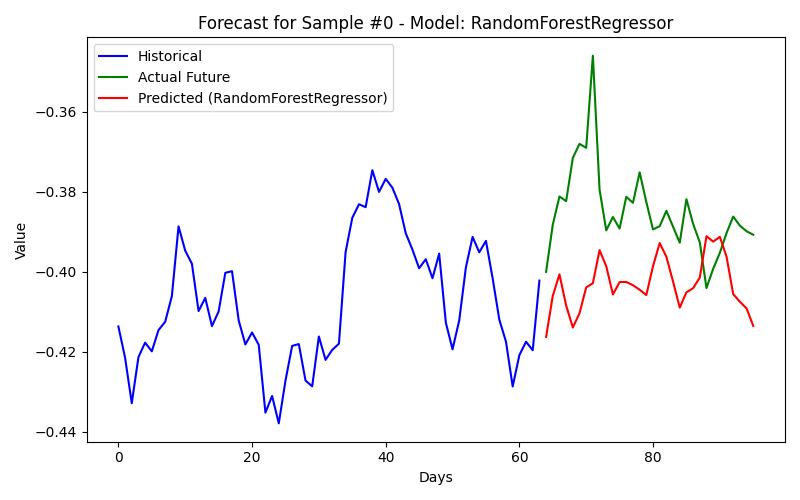
\includegraphics[width=\textwidth]{figures/regressors/RandomForestRegressor/finance_64-32.png}
         \caption{Horizon 64$\to$32}
         \label{fig:RF_finance_64to32}
    \end{subfigure}
    \begin{subfigure}[b]{0.32\textwidth}
         \centering
         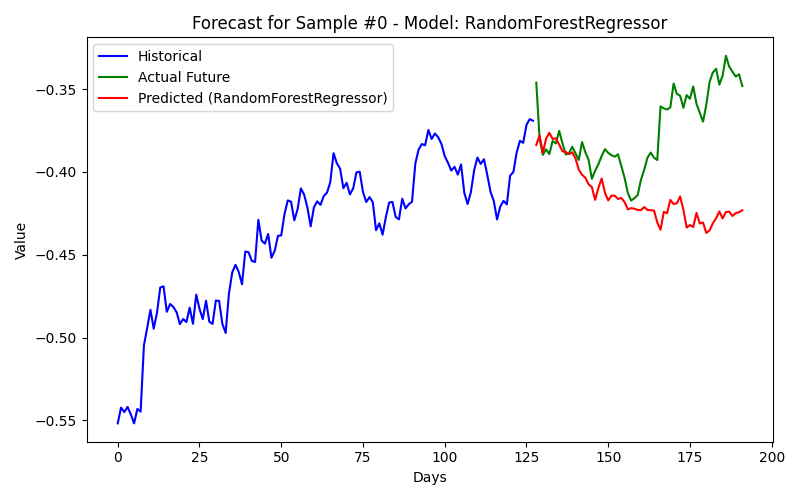
\includegraphics[width=\textwidth]{figures/regressors/RandomForestRegressor/finance_128-64.png}
         \caption{Horizon 128$\to$64}
         \label{fig:RF_finance_128to64}
    \end{subfigure}
    \begin{subfigure}[b]{0.32\textwidth}
         \centering
         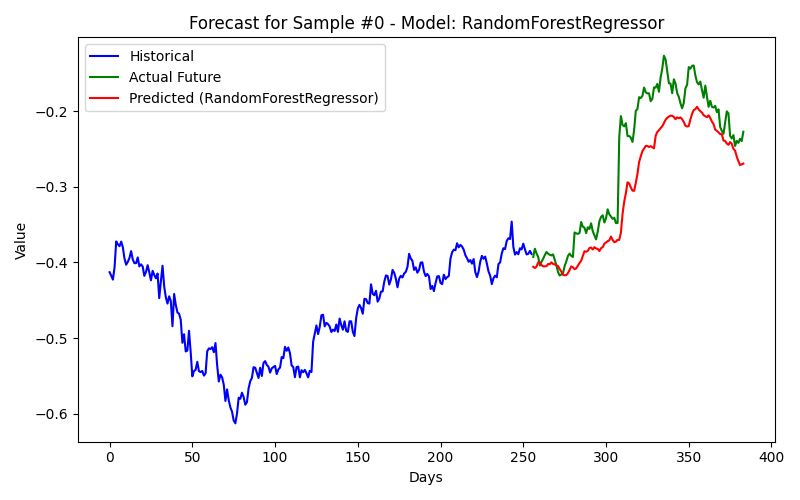
\includegraphics[width=\textwidth]{figures/regressors/RandomForestRegressor/finance_256-128.png}
         \caption{Horizon 256$\to$128}
         \label{fig:RF_finance_256to128}
    \end{subfigure}
    \caption{Random Forest forecasts on the Finance dataset for different horizons.}
    \label{fig:RF_finance_all}
\end{figure}

\subsubsection{Energy Dataset}
\begin{figure}[h!]
    \centering
    \begin{subfigure}[b]{0.32\textwidth}
         \centering
         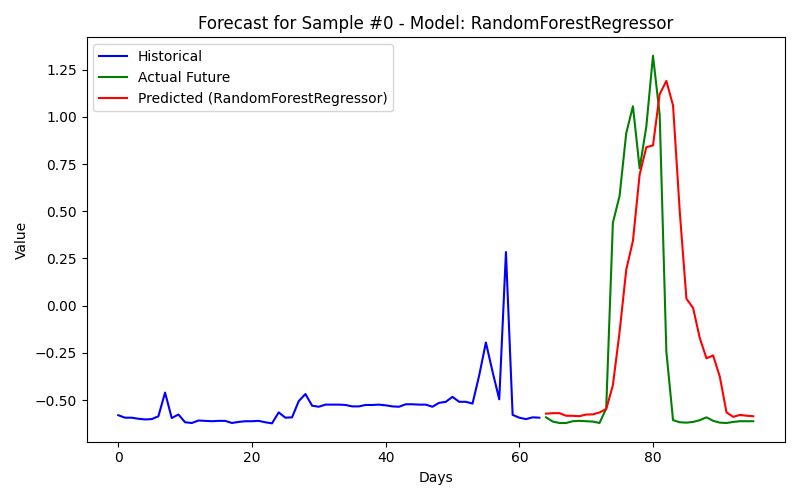
\includegraphics[width=\textwidth]{figures/regressors/RandomForestRegressor/energy_64-32.png}
         \caption{Horizon 64$\to$32}
         \label{fig:RF_energy_64to32}
    \end{subfigure}
    \begin{subfigure}[b]{0.32\textwidth}
         \centering
         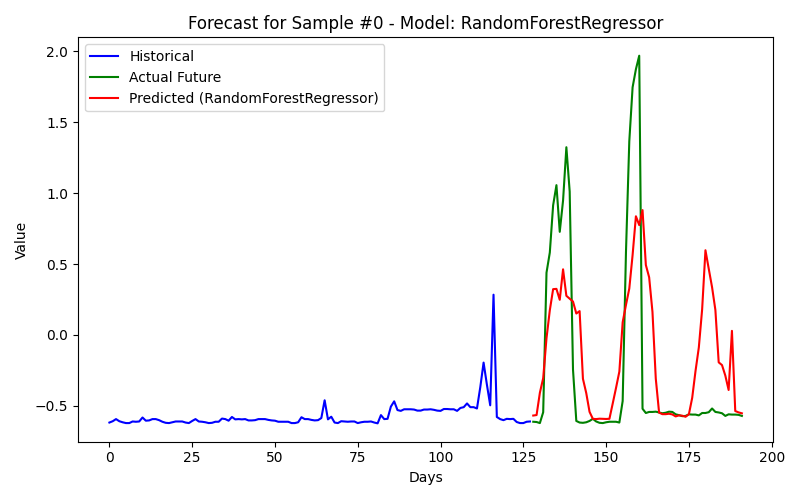
\includegraphics[width=\textwidth]{figures/regressors/RandomForestRegressor/energy_128-64.png}
         \caption{Horizon 128$\to$64}
         \label{fig:RF_energy_128to64}
    \end{subfigure}
    \begin{subfigure}[b]{0.32\textwidth}
         \centering
         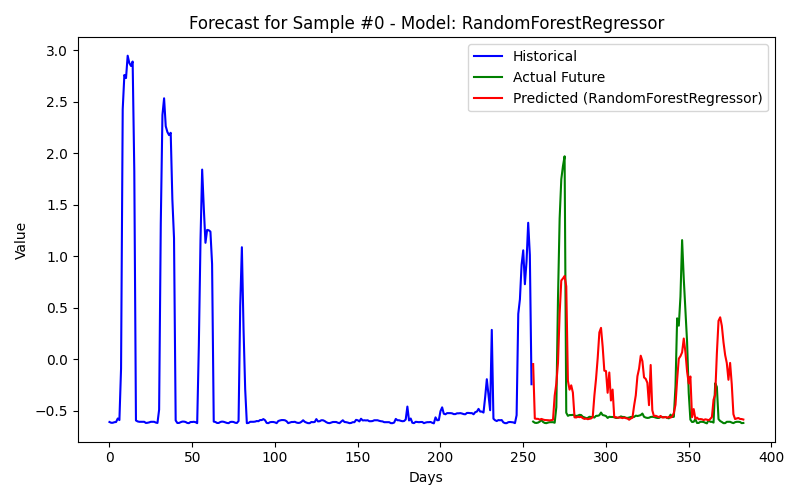
\includegraphics[width=\textwidth]{figures/regressors/RandomForestRegressor/energy_256-128.png}
         \caption{Horizon 256$\to$128}
         \label{fig:RF_energy_256to128}
    \end{subfigure}
    \caption{Random Forest forecasts on the Energy dataset for different horizons.}
    \label{fig:RF_energy_all}
\end{figure}

\subsubsection{Healthcare Dataset}
\begin{figure}[h!]
    \centering
    \begin{subfigure}[b]{0.32\textwidth}
         \centering
         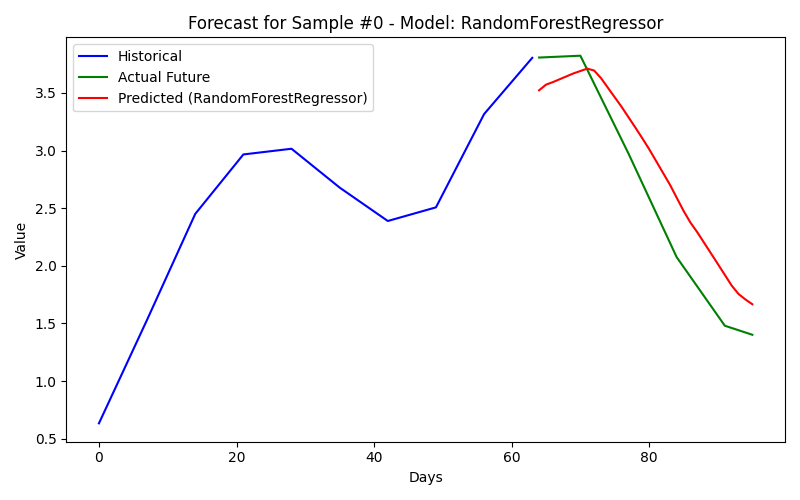
\includegraphics[width=\textwidth]{figures/regressors/RandomForestRegressor/healthcare_64-32.png}
         \caption{Horizon 64$\to$32}
         \label{fig:RF_healthcare_64to32}
    \end{subfigure}
    \begin{subfigure}[b]{0.32\textwidth}
         \centering
         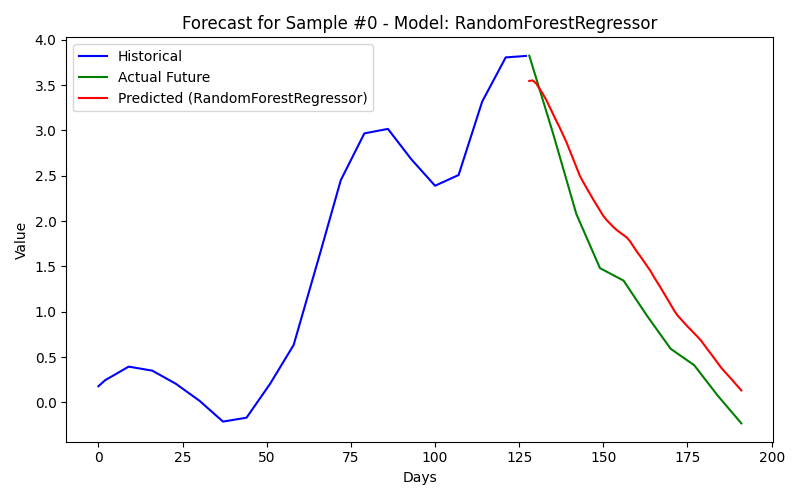
\includegraphics[width=\textwidth]{figures/regressors/RandomForestRegressor/healthcare_128-64.png}
         \caption{Horizon 128$\to$64}
         \label{fig:RF_healthcare_128to64}
    \end{subfigure}
    \begin{subfigure}[b]{0.32\textwidth}
         \centering
         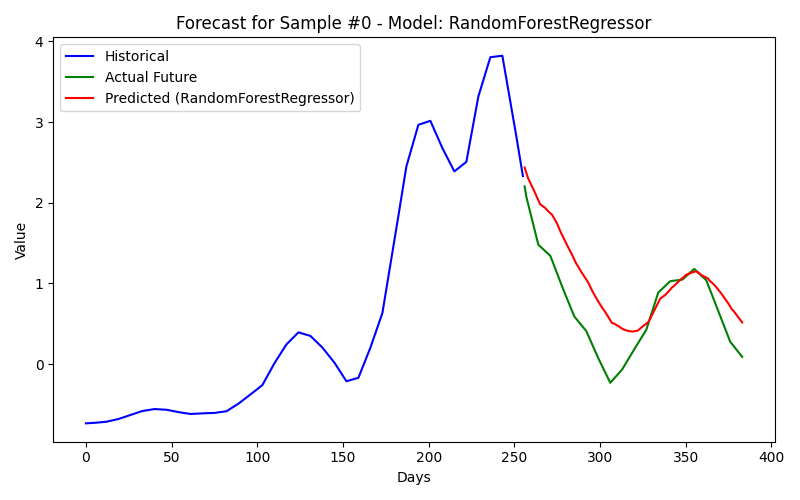
\includegraphics[width=\textwidth]{figures/regressors/RandomForestRegressor/healthcare_256-128.png}
         \caption{Horizon 256$\to$128}
         \label{fig:RF_healthcare_256to128}
    \end{subfigure}
    \caption{Random Forest forecasts on the Healthcare dataset for different horizons.}
    \label{fig:RF_healthcare_all}
\end{figure}

\newpage
%---------------------------------------------------------
\subsection{Extra Trees Regressor}

\subsubsection{Weather Dataset}
\begin{figure}[h!]
    \centering
    \begin{subfigure}[b]{0.32\textwidth}
         \centering
         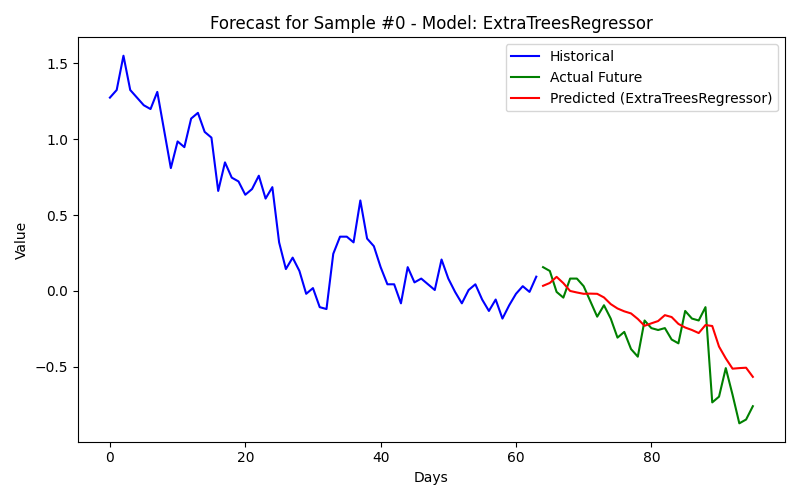
\includegraphics[width=\textwidth]{figures/regressors/ExtraTreesRegressor/weather_64-32.png}
         \caption{Horizon 64$\to$32}
         \label{fig:ET_weather_64to32}
    \end{subfigure}
    \begin{subfigure}[b]{0.32\textwidth}
         \centering
         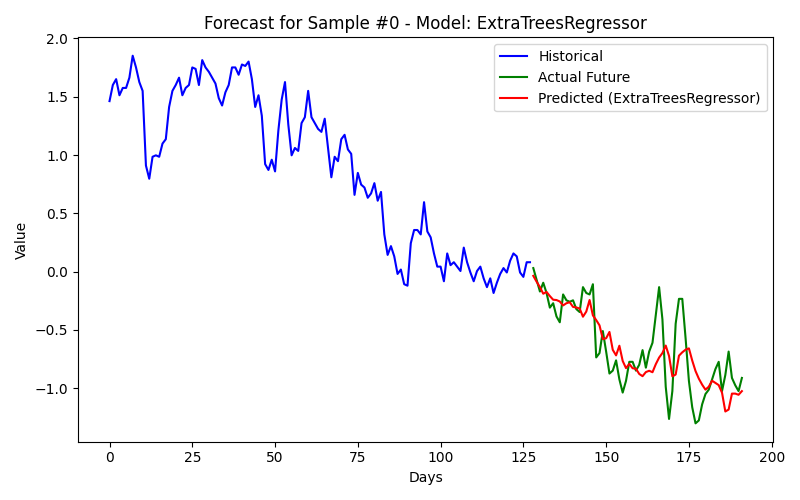
\includegraphics[width=\textwidth]{figures/regressors/ExtraTreesRegressor/weather_128-64.png}
         \caption{Horizon 128$\to$64}
         \label{fig:ET_weather_128to64}
    \end{subfigure}
    \begin{subfigure}[b]{0.32\textwidth}
         \centering
         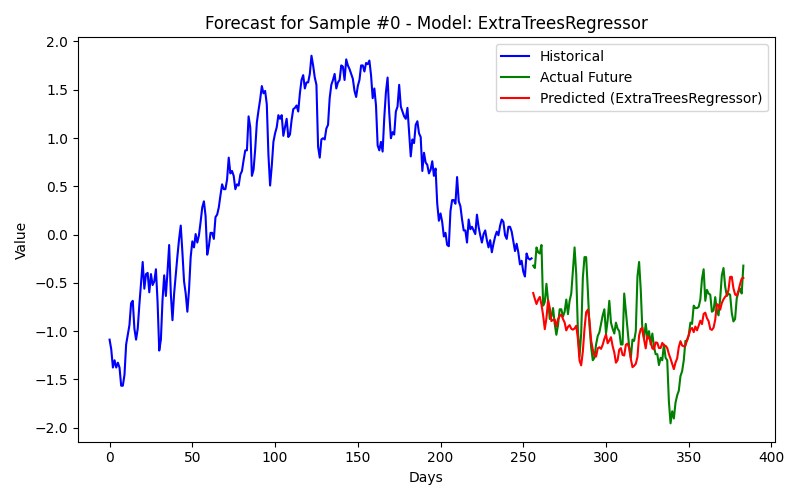
\includegraphics[width=\textwidth]{figures/regressors/ExtraTreesRegressor/weather_256-128.png}
         \caption{Horizon 256$\to$128}
         \label{fig:ET_weather_256to128}
    \end{subfigure}
    \caption{Extra Trees forecasts on the Weather dataset for different horizons.}
    \label{fig:ET_weather_all}
\end{figure}

\subsubsection{Finance Dataset}
\begin{figure}[h!]
    \centering
    \begin{subfigure}[b]{0.32\textwidth}
         \centering
         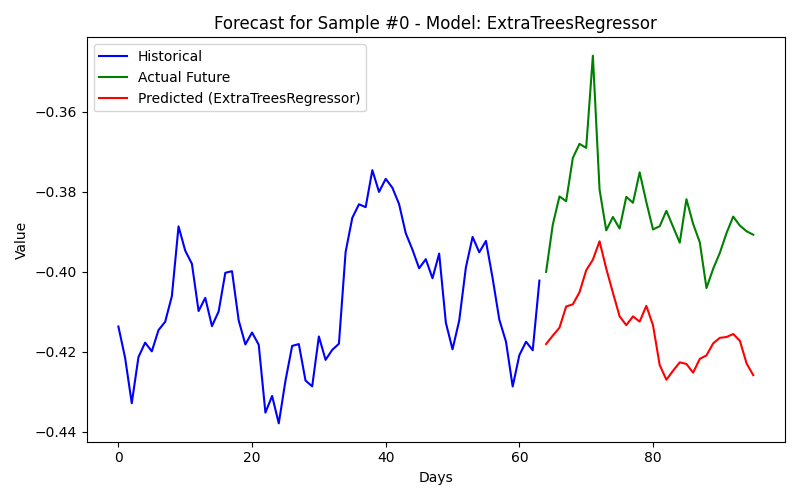
\includegraphics[width=\textwidth]{figures/regressors/ExtraTreesRegressor/finance_64-32.png}
         \caption{Horizon 64$\to$32}
         \label{fig:ET_finance_64to32}
    \end{subfigure}
    \begin{subfigure}[b]{0.32\textwidth}
         \centering
         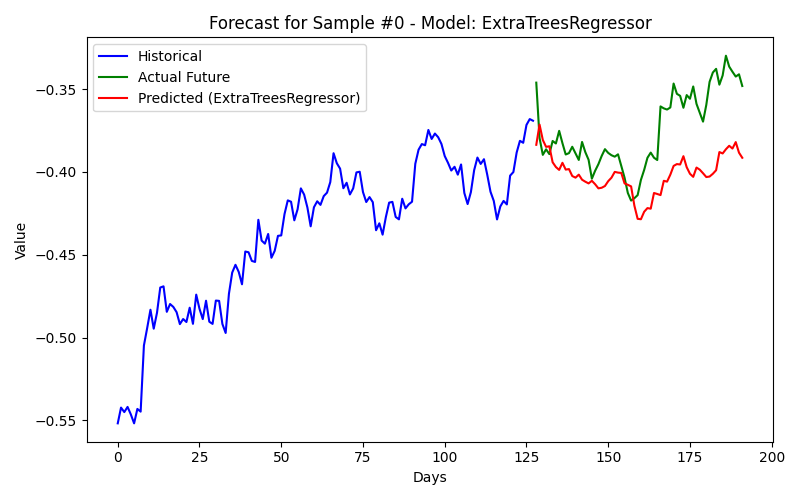
\includegraphics[width=\textwidth]{figures/regressors/ExtraTreesRegressor/finance_128-64.png}
         \caption{Horizon 128$\to$64}
         \label{fig:ET_finance_128to64}
    \end{subfigure}
    \begin{subfigure}[b]{0.32\textwidth}
         \centering
         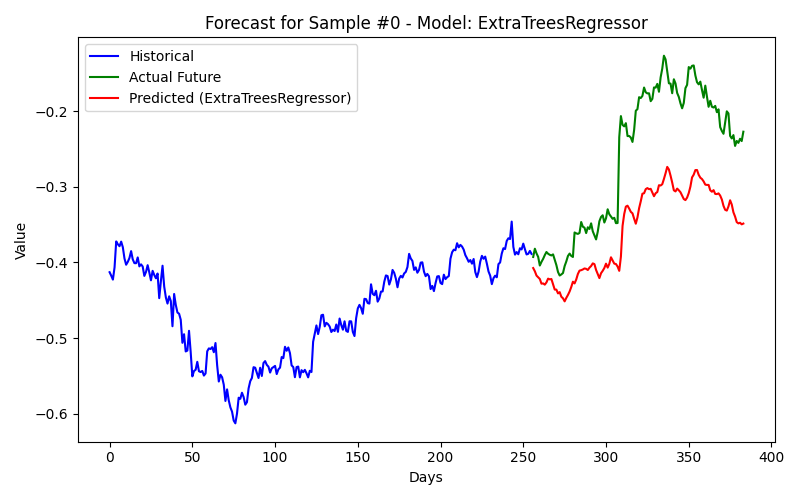
\includegraphics[width=\textwidth]{figures/regressors/ExtraTreesRegressor/finance_256-128.png}
         \caption{Horizon 256$\to$128}
         \label{fig:ET_finance_256to128}
    \end{subfigure}
    \caption{Extra Trees forecasts on the Finance dataset for different horizons.}
    \label{fig:ET_finance_all}
\end{figure}

\subsubsection{Energy Dataset}
\begin{figure}[h!]
    \centering
    \begin{subfigure}[b]{0.32\textwidth}
         \centering
         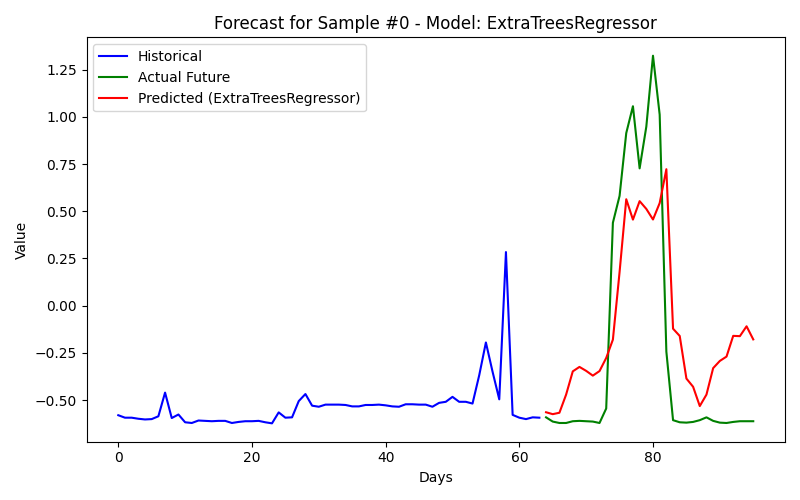
\includegraphics[width=\textwidth]{figures/regressors/ExtraTreesRegressor/energy_64-32.png}
         \caption{Horizon 64$\to$32}
         \label{fig:ET_energy_64to32}
    \end{subfigure}
    \begin{subfigure}[b]{0.32\textwidth}
         \centering
         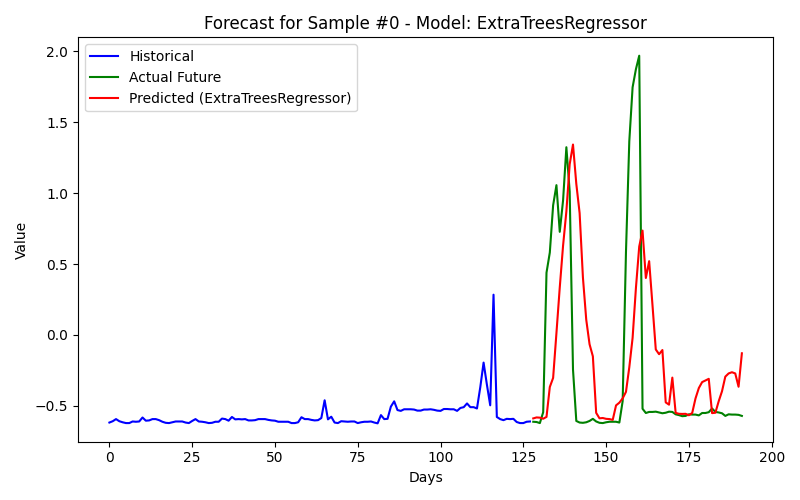
\includegraphics[width=\textwidth]{figures/regressors/ExtraTreesRegressor/energy_128-64.png}
         \caption{Horizon 128$\to$64}
         \label{fig:ET_energy_128to64}
    \end{subfigure}
    \begin{subfigure}[b]{0.32\textwidth}
         \centering
         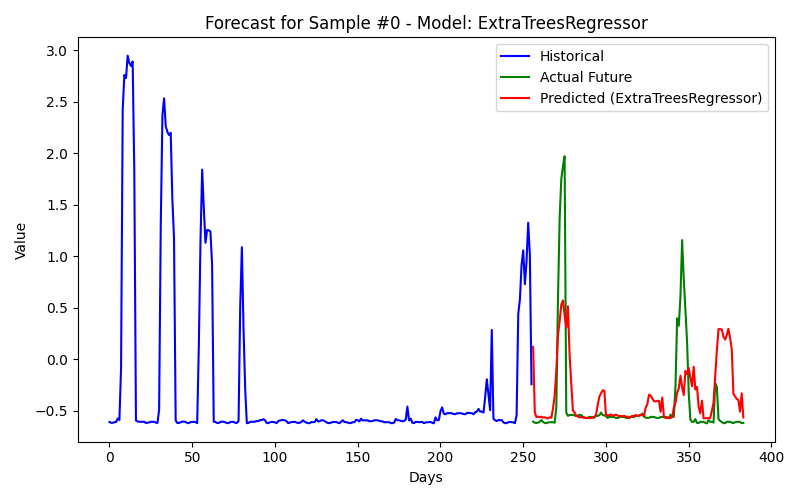
\includegraphics[width=\textwidth]{figures/regressors/ExtraTreesRegressor/energy_256-128.png}
         \caption{Horizon 256$\to$128}
         \label{fig:ET_energy_256to128}
    \end{subfigure}
    \caption{Extra Trees forecasts on the Energy dataset for different horizons.}
    \label{fig:ET_energy_all}
\end{figure}

\subsubsection{Healthcare Dataset}
\begin{figure}[h!]
    \centering
    \begin{subfigure}[b]{0.32\textwidth}
         \centering
         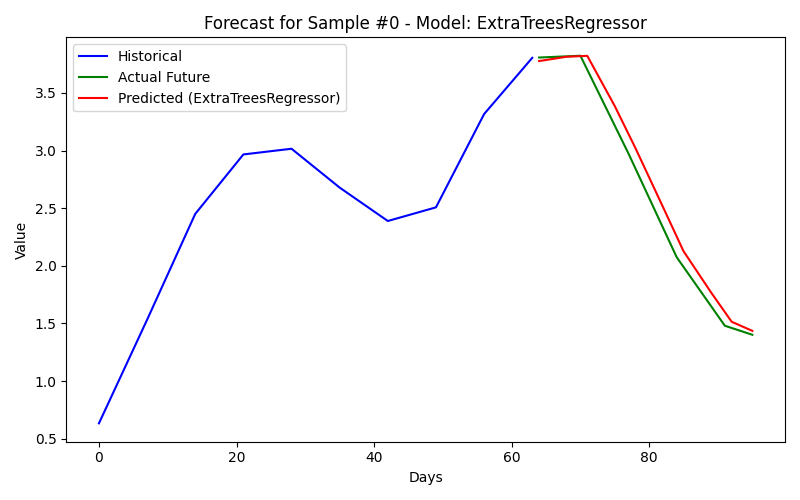
\includegraphics[width=\textwidth]{figures/regressors/ExtraTreesRegressor/healthcare_64-32.png}
         \caption{Horizon 64$\to$32}
         \label{fig:ET_healthcare_64to32}
    \end{subfigure}
    \begin{subfigure}[b]{0.32\textwidth}
         \centering
         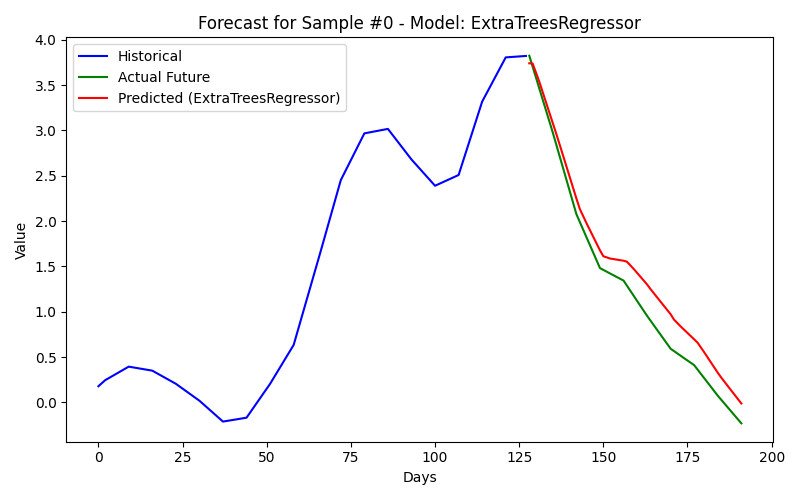
\includegraphics[width=\textwidth]{figures/regressors/ExtraTreesRegressor/healthcare_128-64.png}
         \caption{Horizon 128$\to$64}
         \label{fig:ET_healthcare_128to64}
    \end{subfigure}
    \begin{subfigure}[b]{0.32\textwidth}
         \centering
         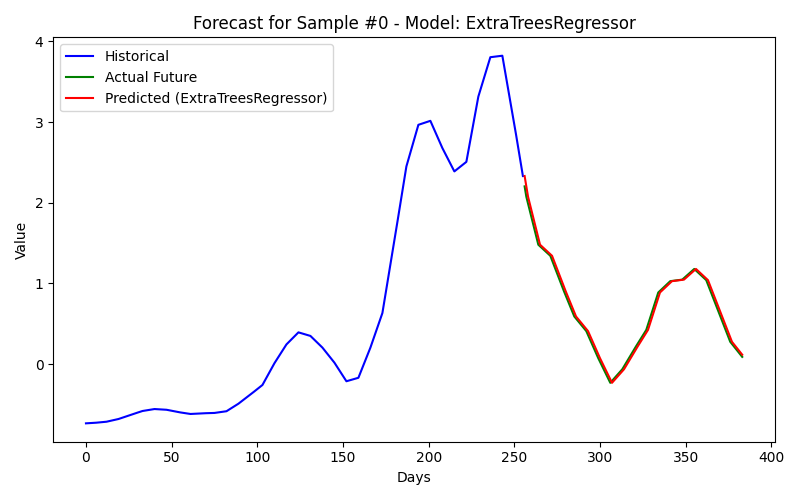
\includegraphics[width=\textwidth]{figures/regressors/ExtraTreesRegressor/healthcare_256-128.png}
         \caption{Horizon 256$\to$128}
         \label{fig:ET_healthcare_256to128}
    \end{subfigure}
    \caption{Extra Trees forecasts on the Healthcare dataset for different horizons.}
    \label{fig:ET_healthcare_all}
\end{figure}

\newpage
%---------------------------------------------------------
\subsection{MLP Regressor}

\subsubsection{Weather Dataset}
\begin{figure}[h!]
    \centering
    \begin{subfigure}[b]{0.32\textwidth}
         \centering
         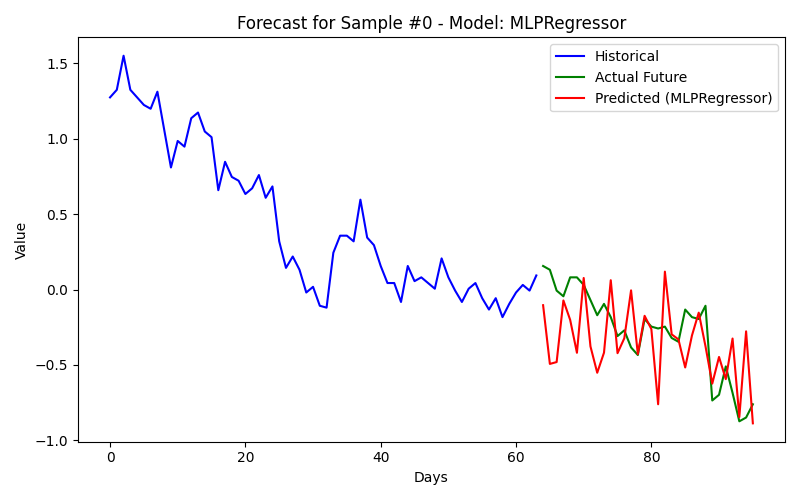
\includegraphics[width=\textwidth]{figures/regressors/MLPRegressor/weather_64-32.png}
         \caption{Horizon 64$\to$32}
         \label{fig:MLP_weather_64to32}
    \end{subfigure}
    \begin{subfigure}[b]{0.32\textwidth}
         \centering
         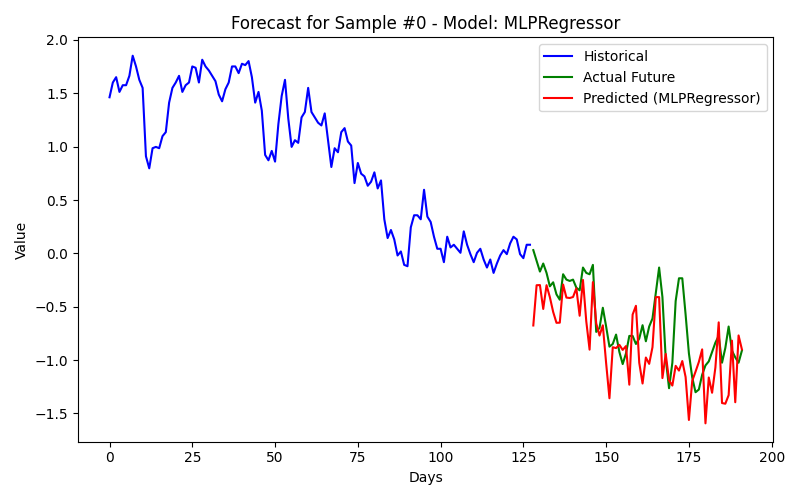
\includegraphics[width=\textwidth]{figures/regressors/MLPRegressor/weather_128-64.png}
         \caption{Horizon 128$\to$64}
         \label{fig:MLP_weather_128to64}
    \end{subfigure}
    \begin{subfigure}[b]{0.32\textwidth}
         \centering
         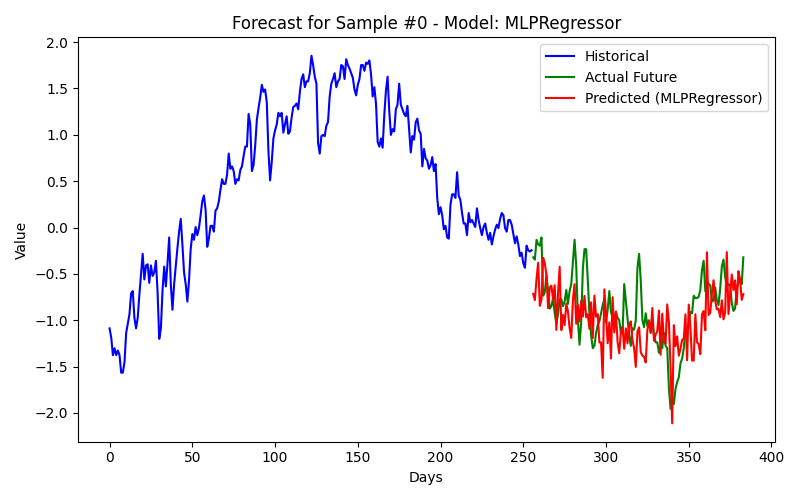
\includegraphics[width=\textwidth]{figures/regressors/MLPRegressor/weather_256-128.png}
         \caption{Horizon 256$\to$128}
         \label{fig:MLP_weather_256to128}
    \end{subfigure}
    \caption{MLP Regressor forecasts on the Weather dataset for different horizons.}
    \label{fig:MLP_weather_all}
\end{figure}

\subsubsection{Finance Dataset}
\begin{figure}[h!]
    \centering
    \begin{subfigure}[b]{0.32\textwidth}
         \centering
         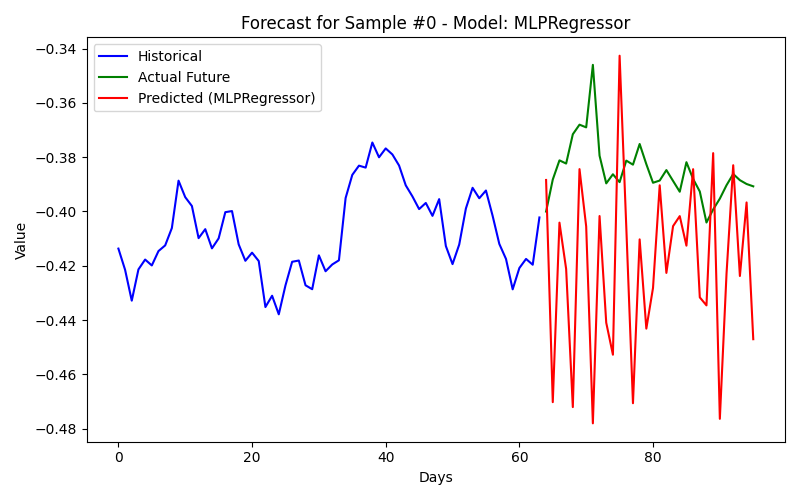
\includegraphics[width=\textwidth]{figures/regressors/MLPRegressor/finance_64-32.png}
         \caption{Horizon 64$\to$32}
         \label{fig:MLP_finance_64to32}
    \end{subfigure}
    \begin{subfigure}[b]{0.32\textwidth}
         \centering
         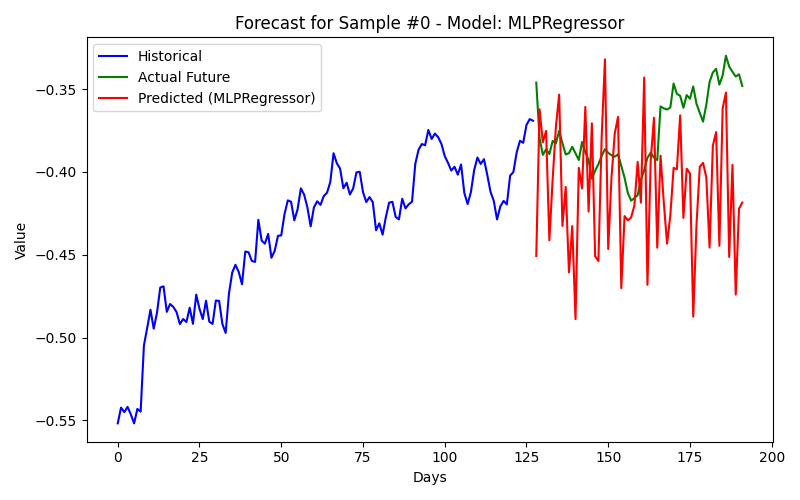
\includegraphics[width=\textwidth]{figures/regressors/MLPRegressor/finance_128-64.png}
         \caption{Horizon 128$\to$64}
         \label{fig:MLP_finance_128to64}
    \end{subfigure}
    \begin{subfigure}[b]{0.32\textwidth}
         \centering
         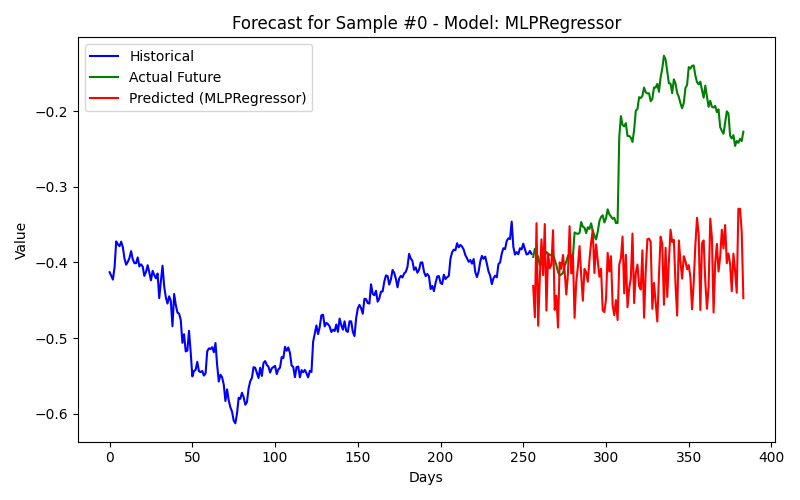
\includegraphics[width=\textwidth]{figures/regressors/MLPRegressor/finance_256-128.png}
         \caption{Horizon 256$\to$128}
         \label{fig:MLP_finance_256to128}
    \end{subfigure}
    \caption{MLP Regressor forecasts on the Finance dataset for different horizons.}
    \label{fig:MLP_finance_all}
\end{figure}

\subsubsection{Energy Dataset}
\begin{figure}[h!]
    \centering
    \begin{subfigure}[b]{0.32\textwidth}
         \centering
         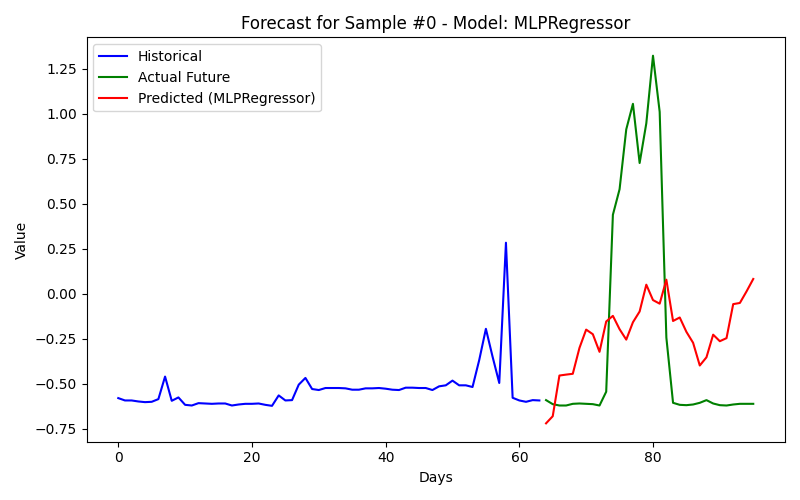
\includegraphics[width=\textwidth]{figures/regressors/MLPRegressor/energy_64-32.png}
         \caption{Horizon 64$\to$32}
         \label{fig:MLP_energy_64to32}
    \end{subfigure}
    \begin{subfigure}[b]{0.32\textwidth}
         \centering
         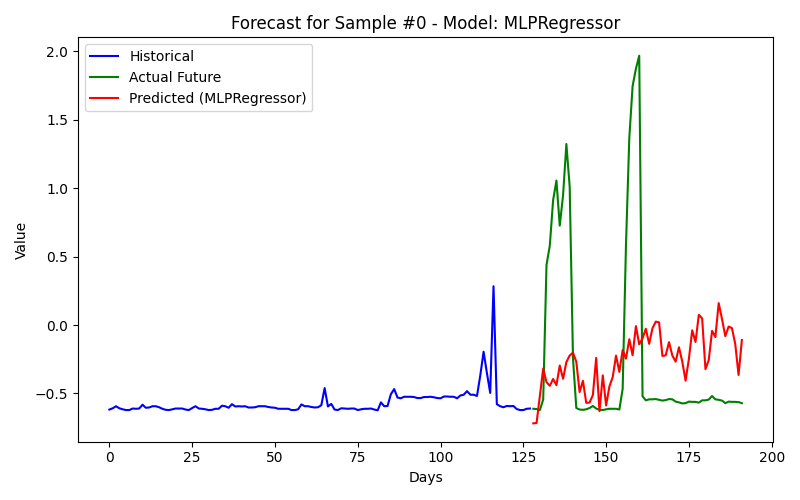
\includegraphics[width=\textwidth]{figures/regressors/MLPRegressor/energy_128-64.png}
         \caption{Horizon 128$\to$64}
         \label{fig:MLP_energy_128to64}
    \end{subfigure}
    \begin{subfigure}[b]{0.32\textwidth}
         \centering
         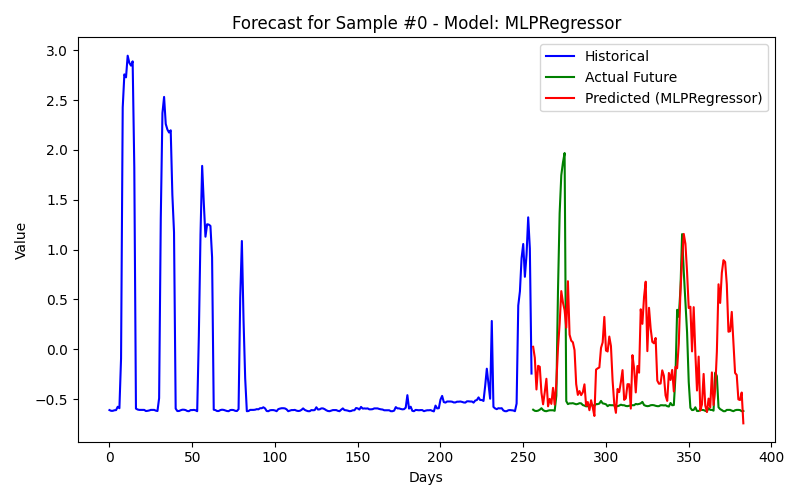
\includegraphics[width=\textwidth]{figures/regressors/MLPRegressor/energy_256-128.png}
         \caption{Horizon 256$\to$128}
         \label{fig:MLP_energy_256to128}
    \end{subfigure}
    \caption{MLP Regressor forecasts on the Energy dataset for different horizons.}
    \label{fig:MLP_energy_all}
\end{figure}

\subsubsection{Healthcare Dataset}
\begin{figure}[h!]
    \centering
    \begin{subfigure}[b]{0.32\textwidth}
         \centering
         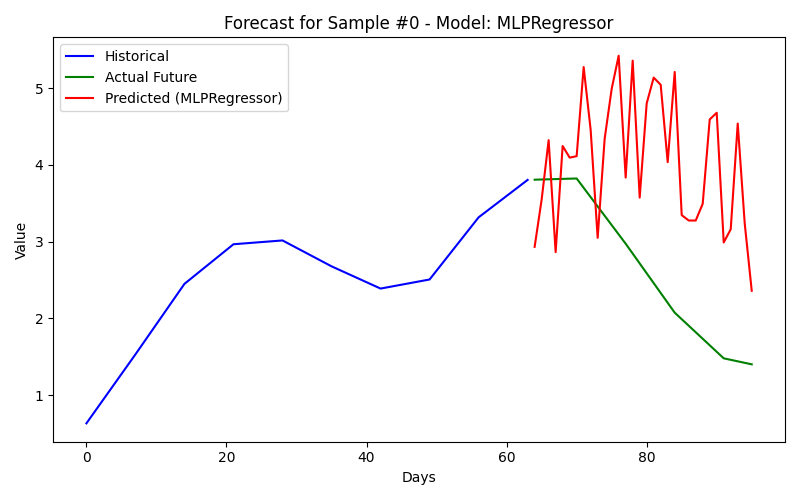
\includegraphics[width=\textwidth]{figures/regressors/MLPRegressor/healthcare_64-32.png}
         \caption{Horizon 64$\to$32}
         \label{fig:MLP_healthcare_64to32}
    \end{subfigure}
    \begin{subfigure}[b]{0.32\textwidth}
         \centering
         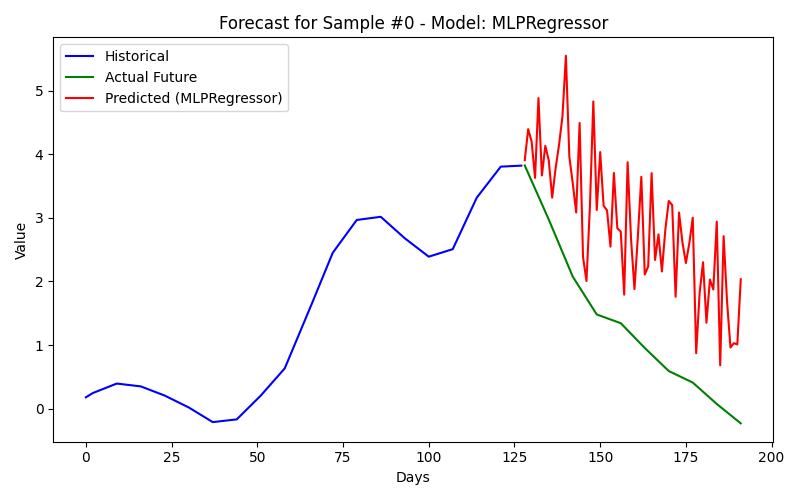
\includegraphics[width=\textwidth]{figures/regressors/MLPRegressor/healthcare_128-64.png}
         \caption{Horizon 128$\to$64}
         \label{fig:MLP_healthcare_128to64}
    \end{subfigure}
    \begin{subfigure}[b]{0.32\textwidth}
         \centering
         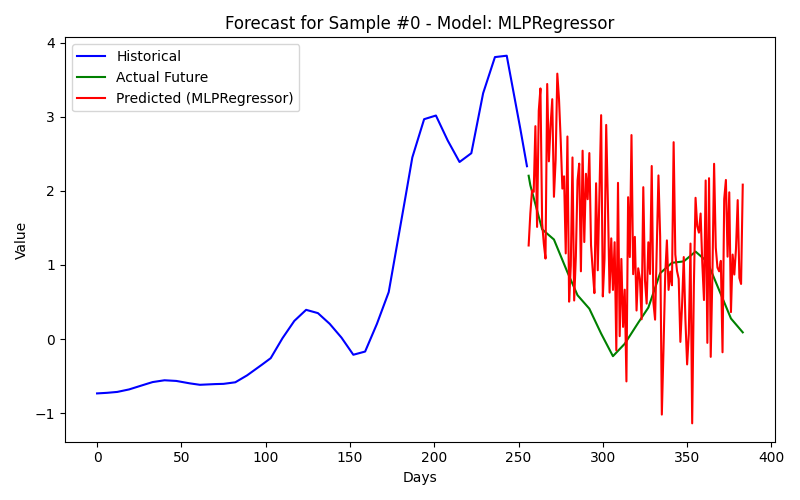
\includegraphics[width=\textwidth]{figures/regressors/MLPRegressor/healthcare_256-128.png}
         \caption{Horizon 256$\to$128}
         \label{fig:MLP_healthcare_256to128}
    \end{subfigure}
    \caption{MLP Regressor forecasts on the Healthcare dataset for different horizons.}
    \label{fig:MLP_healthcare_all}
\end{figure}

\newpage
%---------------------------------------------------------
\subsection{HistGradientBoosting Regressor}

\subsubsection{Weather Dataset}
\begin{figure}[h!]
    \centering
    \begin{subfigure}[b]{0.32\textwidth}
         \centering
         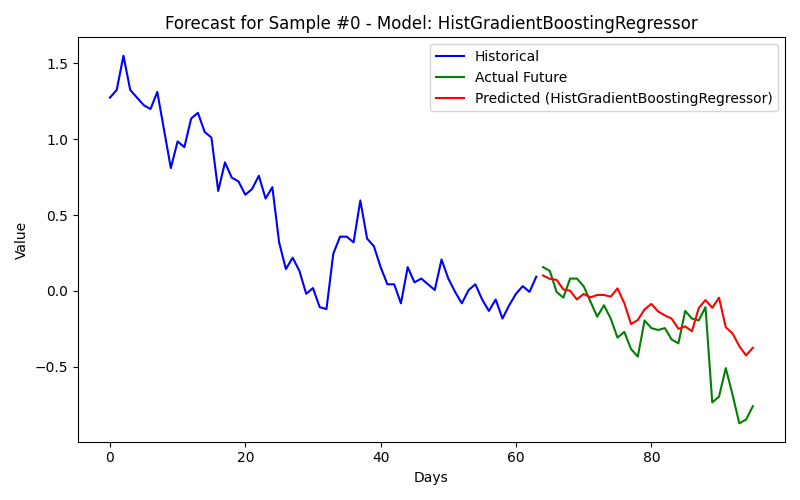
\includegraphics[width=\textwidth]{figures/regressors/HistGradientBoostingRegressor/weather_64-32.png}
         \caption{Horizon 64$\to$32}
         \label{fig:HGB_weather_64to32}
    \end{subfigure}
    \begin{subfigure}[b]{0.32\textwidth}
         \centering
         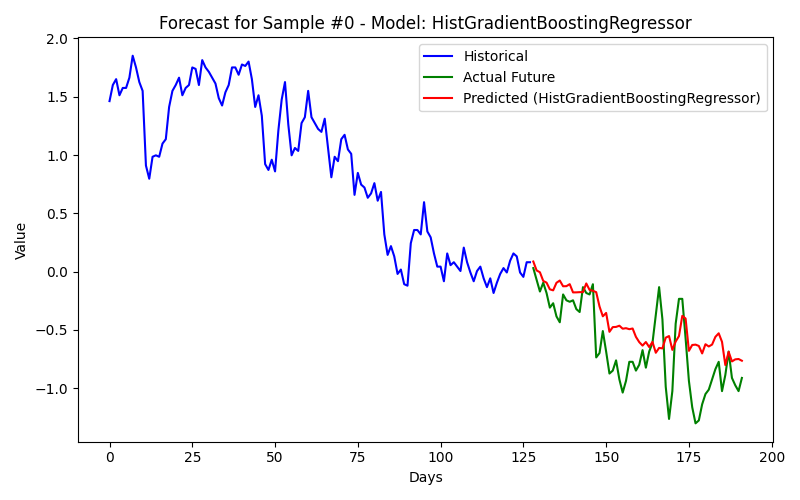
\includegraphics[width=\textwidth]{figures/regressors/HistGradientBoostingRegressor/weather_128-64.png}
         \caption{Horizon 128$\to$64}
         \label{fig:HGB_weather_128to64}
    \end{subfigure}
    \begin{subfigure}[b]{0.32\textwidth}
         \centering
         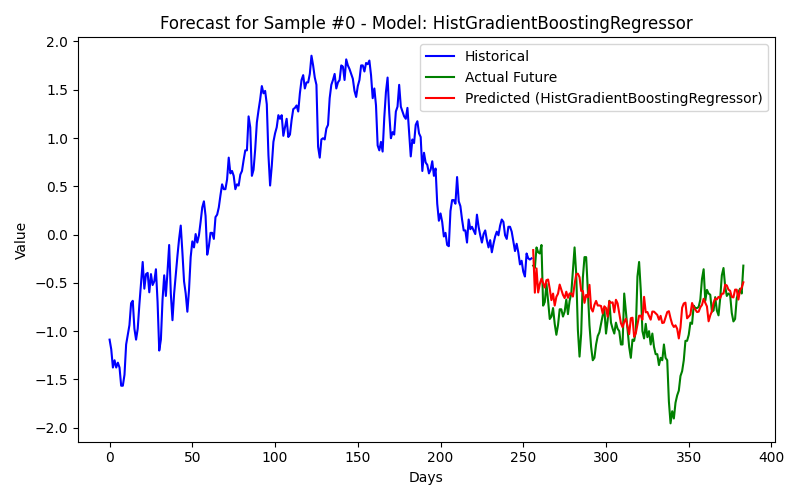
\includegraphics[width=\textwidth]{figures/regressors/HistGradientBoostingRegressor/weather_256-128.png}
         \caption{Horizon 256$\to$128}
         \label{fig:HGB_weather_256to128}
    \end{subfigure}
    \caption{HistGradientBoosting forecasts on the Weather dataset for different horizons.}
    \label{fig:HGB_weather_all}
\end{figure}

\subsubsection{Finance Dataset}
\begin{figure}[h!]
    \centering
    \begin{subfigure}[b]{0.32\textwidth}
         \centering
         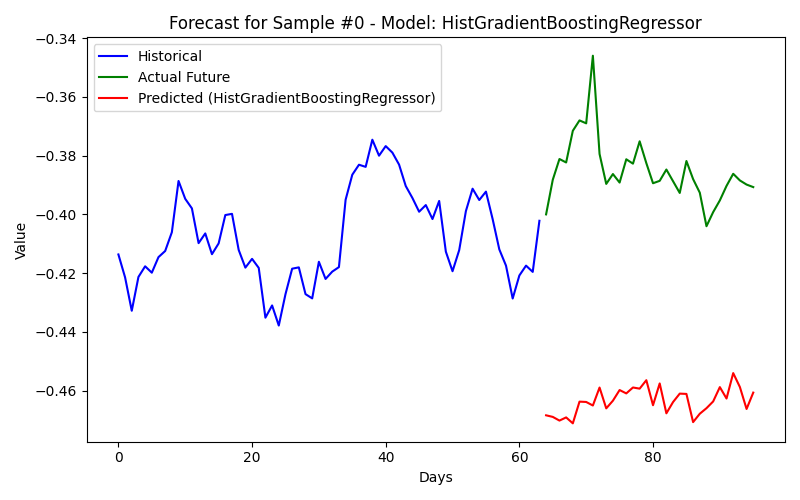
\includegraphics[width=\textwidth]{figures/regressors/HistGradientBoostingRegressor/finance_64-32.png}
         \caption{Horizon 64$\to$32}
         \label{fig:HGB_finance_64to32}
    \end{subfigure}
    \begin{subfigure}[b]{0.32\textwidth}
         \centering
         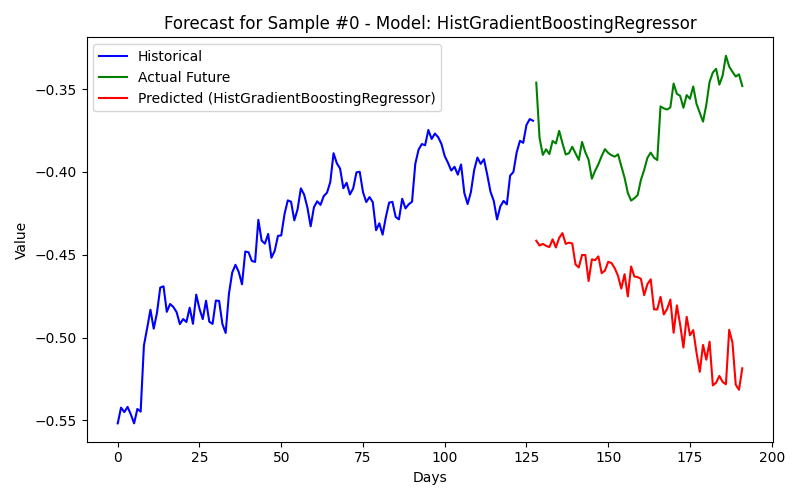
\includegraphics[width=\textwidth]{figures/regressors/HistGradientBoostingRegressor/finance_128-64.png}
         \caption{Horizon 128$\to$64}
         \label{fig:HGB_finance_128to64}
    \end{subfigure}
    \begin{subfigure}[b]{0.32\textwidth}
         \centering
         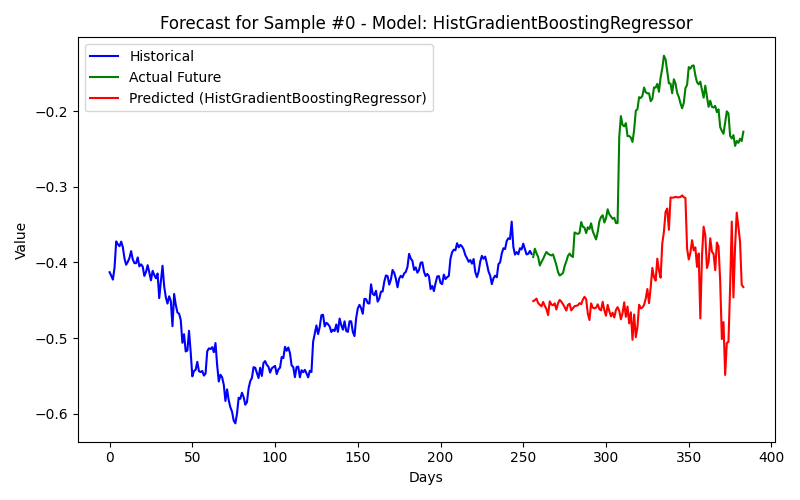
\includegraphics[width=\textwidth]{figures/regressors/HistGradientBoostingRegressor/finance_256-128.png}
         \caption{Horizon 256$\to$128}
         \label{fig:HGB_finance_256to128}
    \end{subfigure}
    \caption{HistGradientBoosting forecasts on the Finance dataset for different horizons.}
    \label{fig:HGB_finance_all}
\end{figure}

\subsubsection{Energy Dataset}
\begin{figure}[h!]
    \centering
    \begin{subfigure}[b]{0.32\textwidth}
         \centering
         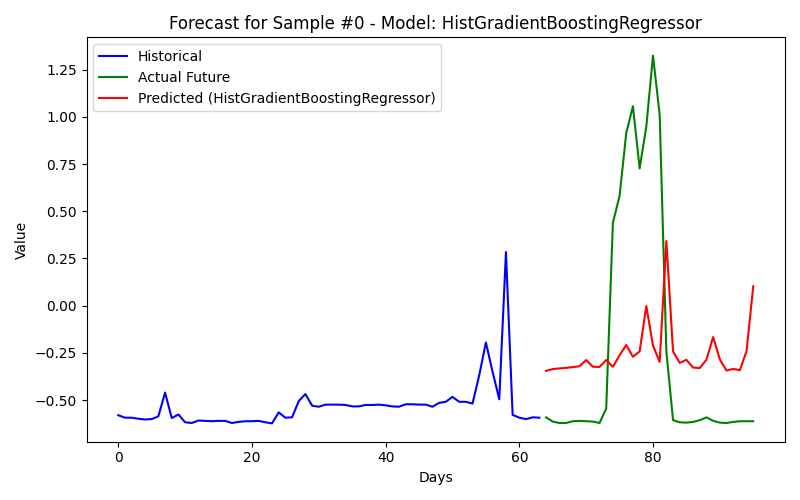
\includegraphics[width=\textwidth]{figures/regressors/HistGradientBoostingRegressor/energy_64-32.png}
         \caption{Horizon 64$\to$32}
         \label{fig:HGB_energy_64to32}
    \end{subfigure}
    \begin{subfigure}[b]{0.32\textwidth}
         \centering
         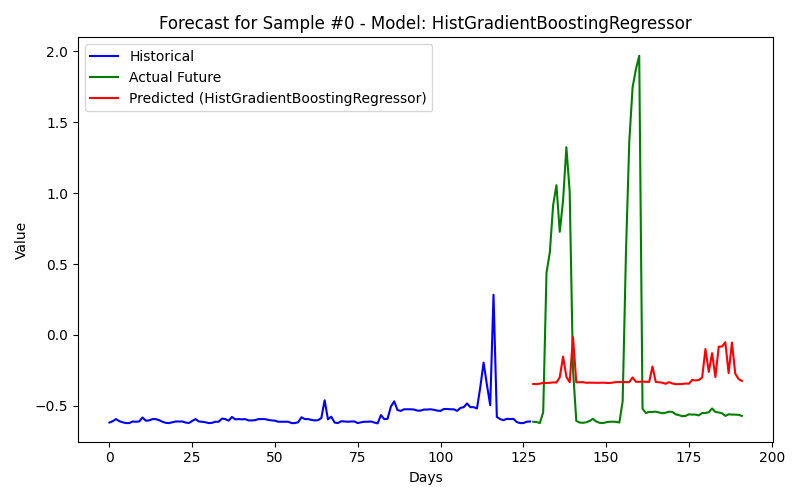
\includegraphics[width=\textwidth]{figures/regressors/HistGradientBoostingRegressor/energy_128-64.png}
         \caption{Horizon 128$\to$64}
         \label{fig:HGB_energy_128to64}
    \end{subfigure}
    \begin{subfigure}[b]{0.32\textwidth}
         \centering
         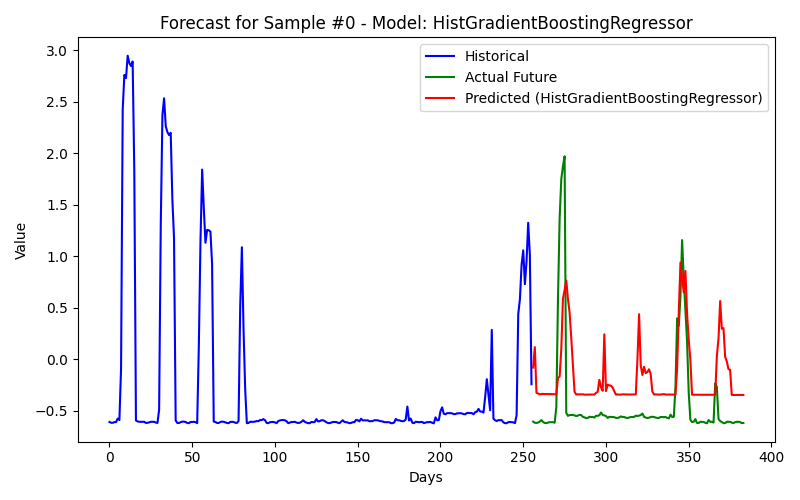
\includegraphics[width=\textwidth]{figures/regressors/HistGradientBoostingRegressor/energy_256-128.png}
         \caption{Horizon 256$\to$128}
         \label{fig:HGB_energy_256to128}
    \end{subfigure}
    \caption{HistGradientBoosting forecasts on the Energy dataset for different horizons.}
    \label{fig:HGB_energy_all}
\end{figure}

\subsubsection{Healthcare Dataset}
\begin{figure}[h!]
    \centering
    \begin{subfigure}[b]{0.32\textwidth}
         \centering
         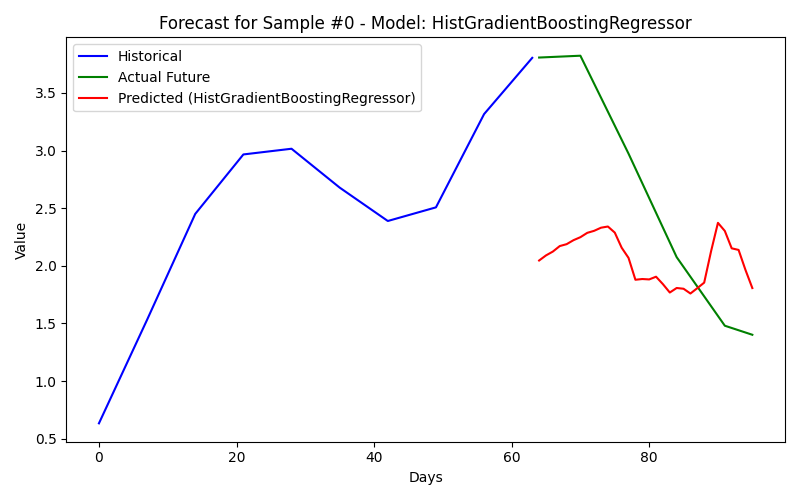
\includegraphics[width=\textwidth]{figures/regressors/HistGradientBoostingRegressor/healthcare_64-32.png}
         \caption{Horizon 64$\to$32}
         \label{fig:HGB_healthcare_64to32}
    \end{subfigure}
    \begin{subfigure}[b]{0.32\textwidth}
         \centering
         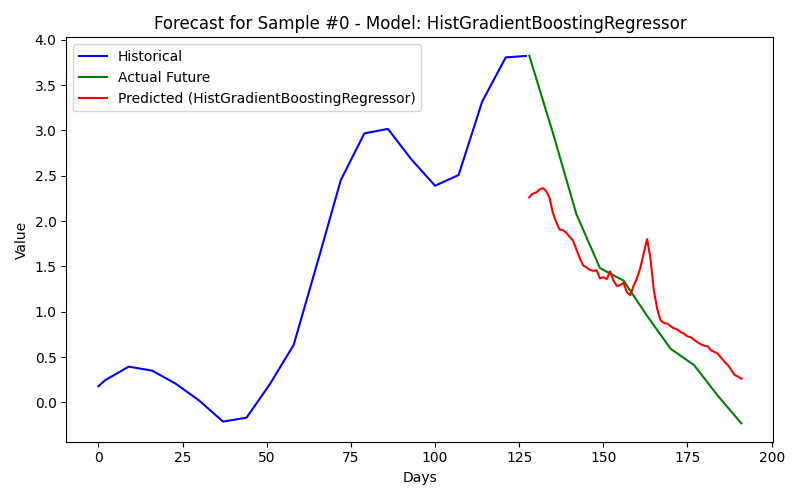
\includegraphics[width=\textwidth]{figures/regressors/HistGradientBoostingRegressor/healthcare_128-64.png}
         \caption{Horizon 128$\to$64}
         \label{fig:HGB_healthcare_128to64}
    \end{subfigure}
    \begin{subfigure}[b]{0.32\textwidth}
         \centering
         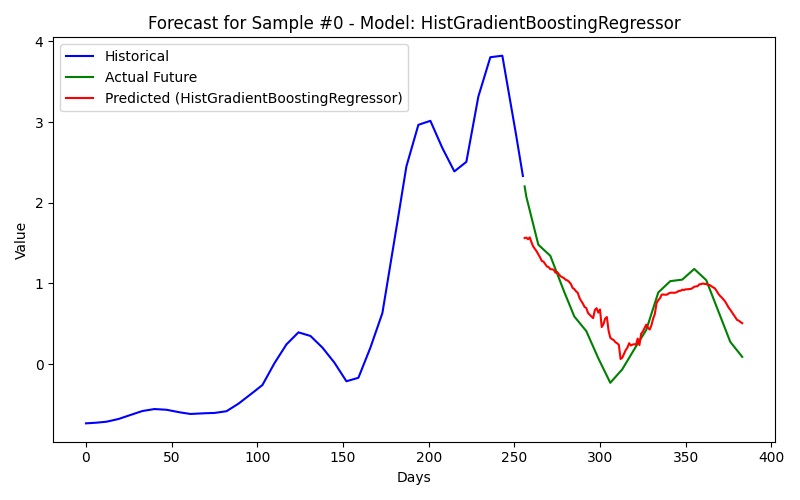
\includegraphics[width=\textwidth]{figures/regressors/HistGradientBoostingRegressor/healthcare_256-128.png}
         \caption{Horizon 256$\to$128}
         \label{fig:HGB_healthcare_256to128}
    \end{subfigure}
    \caption{HistGradientBoosting forecasts on the Healthcare dataset for different horizons.}
    \label{fig:HGB_healthcare_all}
\end{figure}

\newpage
%---------------------------------------------------------
\subsection{Linear SVR}

\subsubsection{Weather Dataset}
\begin{figure}[h!]
    \centering
    \begin{subfigure}[b]{0.32\textwidth}
         \centering
         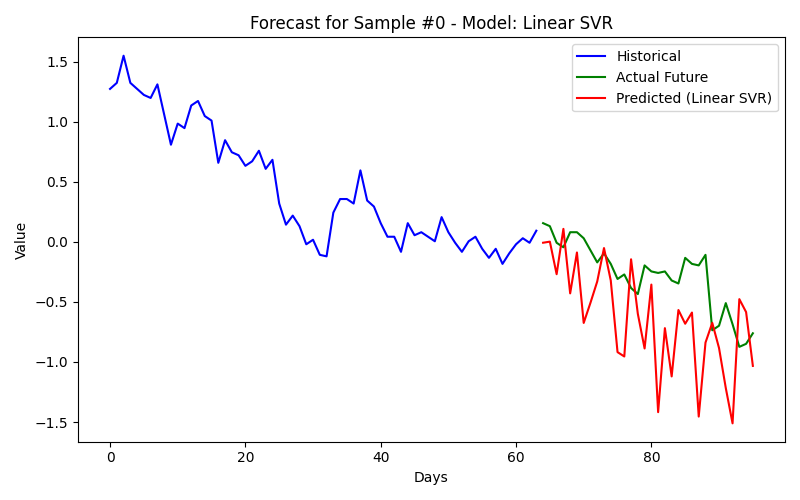
\includegraphics[width=\textwidth]{figures/regressors/Linear SVR/weather_64-32.png}
         \caption{Horizon 64$\to$32}
         \label{fig:SVR_weather_64to32}
    \end{subfigure}
    \begin{subfigure}[b]{0.32\textwidth}
         \centering
         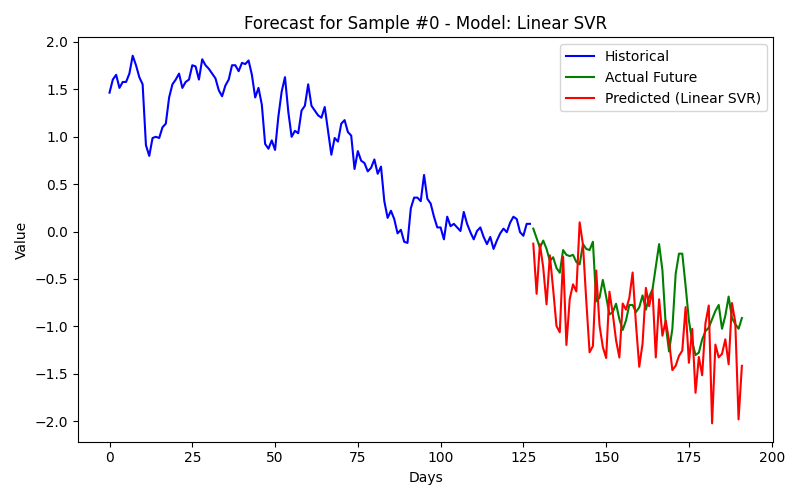
\includegraphics[width=\textwidth]{figures/regressors/Linear SVR/weather_128-64.png}
         \caption{Horizon 128$\to$64}
         \label{fig:SVR_weather_128to64}
    \end{subfigure}
    \begin{subfigure}[b]{0.32\textwidth}
         \centering
         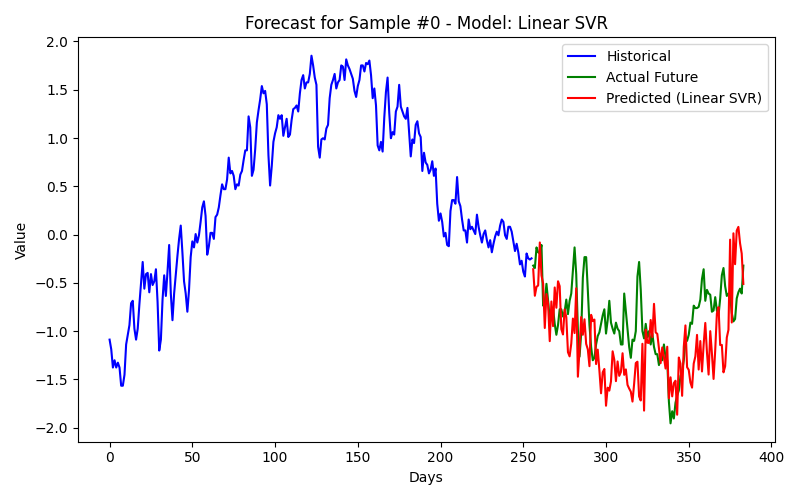
\includegraphics[width=\textwidth]{figures/regressors/Linear SVR/weather_256-128.png}
         \caption{Horizon 256$\to$128}
         \label{fig:SVR_weather_256to128}
    \end{subfigure}
    \caption{Linear SVR forecasts on the Weather dataset for different horizons.}
    \label{fig:SVR_weather_all}
\end{figure}

\subsubsection{Finance Dataset}
\begin{figure}[h!]
    \centering
    \begin{subfigure}[b]{0.32\textwidth}
         \centering
         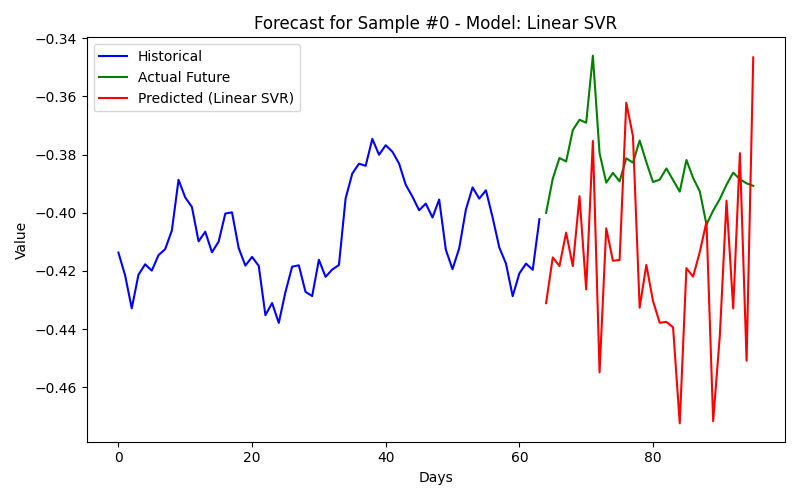
\includegraphics[width=\textwidth]{figures/regressors/Linear SVR/finance_64-32.png}
         \caption{Horizon 64$\to$32}
         \label{fig:SVR_finance_64to32}
    \end{subfigure}
    \begin{subfigure}[b]{0.32\textwidth}
         \centering
         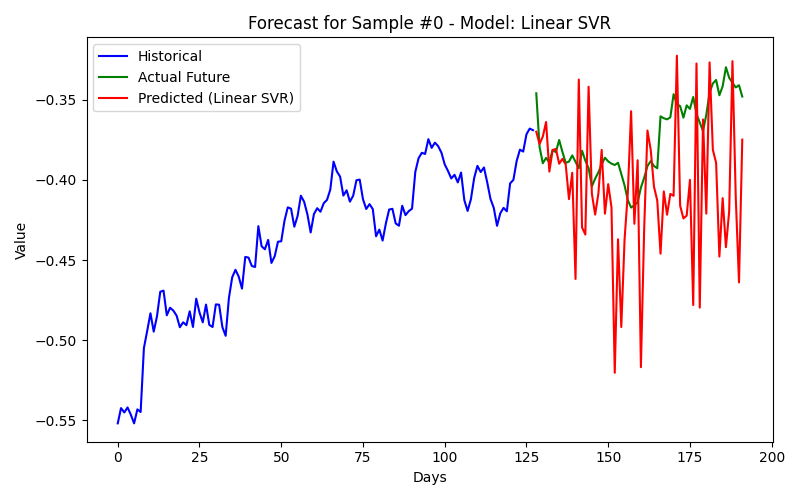
\includegraphics[width=\textwidth]{figures/regressors/Linear SVR/finance_128-64.png}
         \caption{Horizon 128$\to$64}
         \label{fig:SVR_finance_128to64}
    \end{subfigure}
    \begin{subfigure}[b]{0.32\textwidth}
         \centering
         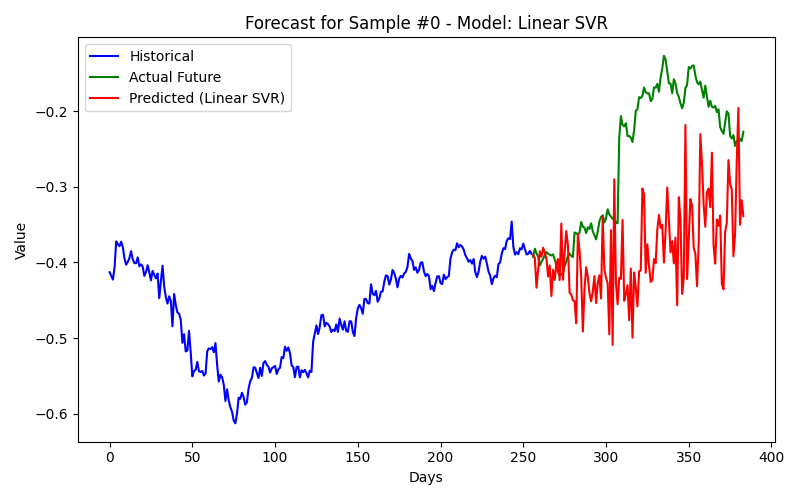
\includegraphics[width=\textwidth]{figures/regressors/Linear SVR/finance_256-128.png}
         \caption{Horizon 256$\to$128}
         \label{fig:SVR_finance_256to128}
    \end{subfigure}
    \caption{Linear SVR forecasts on the Finance dataset for different horizons.}
    \label{fig:SVR_finance_all}
\end{figure}

\subsubsection{Energy Dataset}
\begin{figure}[h!]
    \centering
    \begin{subfigure}[b]{0.32\textwidth}
         \centering
         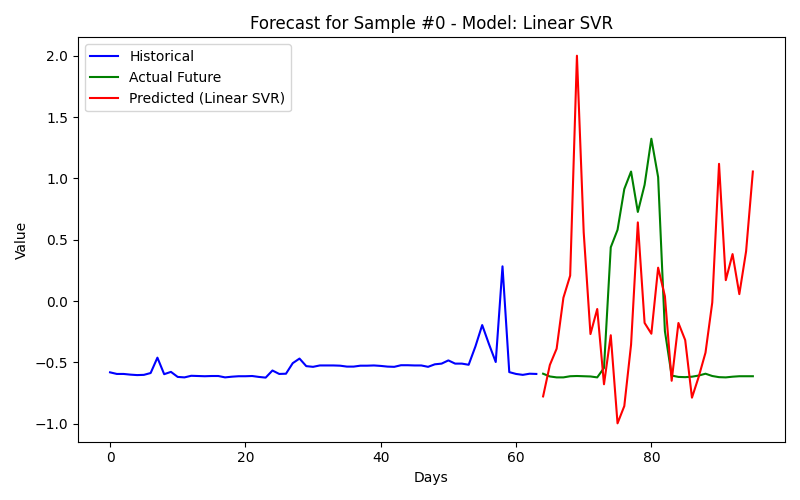
\includegraphics[width=\textwidth]{figures/regressors/Linear SVR/energy_64-32.png}
         \caption{Horizon 64$\to$32}
         \label{fig:SVR_energy_64to32}
    \end{subfigure}
    \begin{subfigure}[b]{0.32\textwidth}
         \centering
         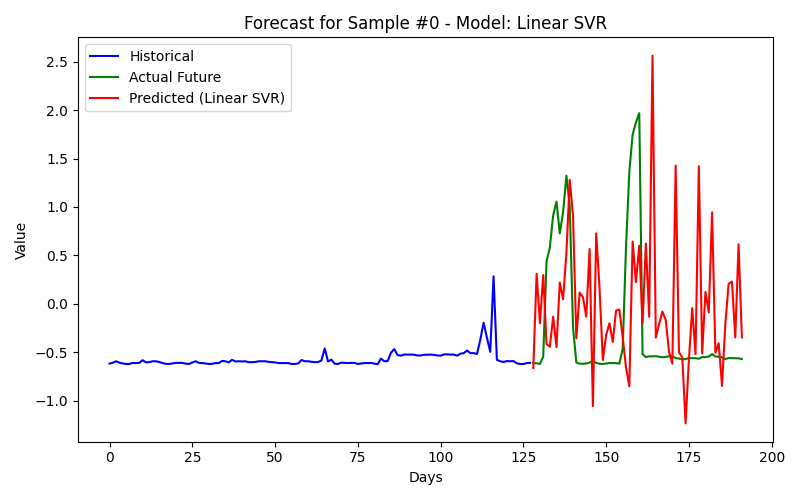
\includegraphics[width=\textwidth]{figures/regressors/Linear SVR/energy_128-64.png}
         \caption{Horizon 128$\to$64}
         \label{fig:SVR_energy_128to64}
    \end{subfigure}
    \begin{subfigure}[b]{0.32\textwidth}
         \centering
         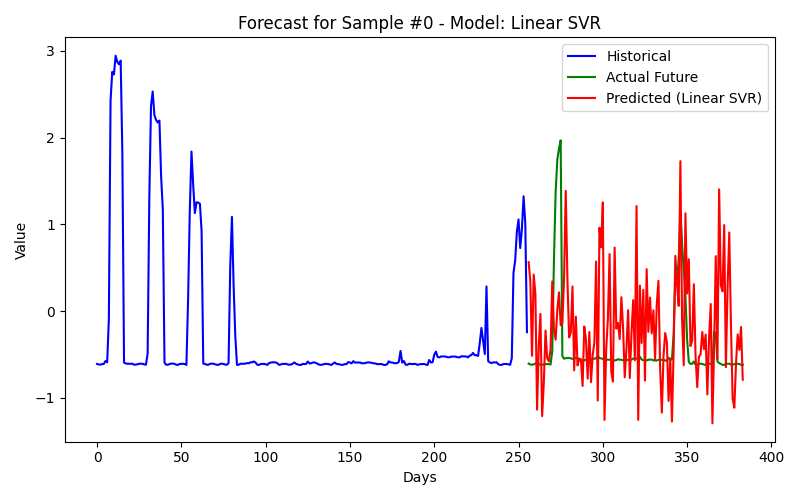
\includegraphics[width=\textwidth]{figures/regressors/Linear SVR/energy_256-128.png}
         \caption{Horizon 256$\to$128}
         \label{fig:SVR_energy_256to128}
    \end{subfigure}
    \caption{Linear SVR forecasts on the Energy dataset for different horizons.}
    \label{fig:SVR_energy_all}
\end{figure}

\subsubsection{Healthcare Dataset}
\begin{figure}[h!]
    \centering
    \begin{subfigure}[b]{0.32\textwidth}
         \centering
         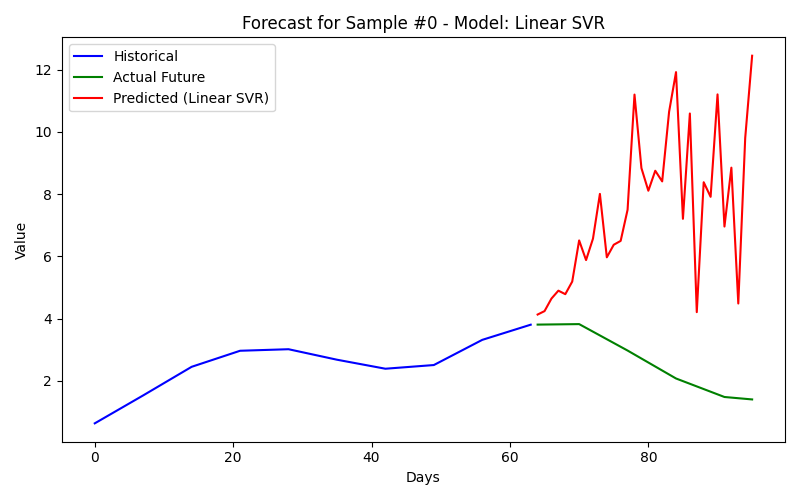
\includegraphics[width=\textwidth]{figures/regressors/Linear SVR/healthcare_64-32.png}
         \caption{Horizon 64$\to$32}
         \label{fig:SVR_healthcare_64to32}
    \end{subfigure}
    \begin{subfigure}[b]{0.32\textwidth}
         \centering
         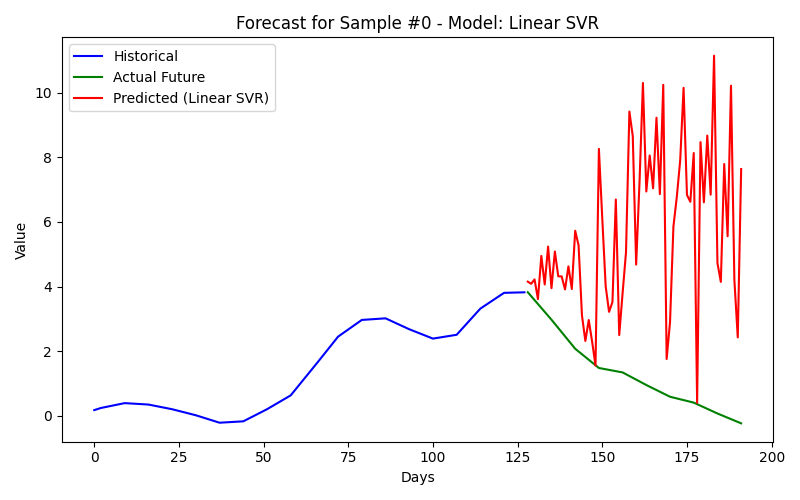
\includegraphics[width=\textwidth]{figures/regressors/Linear SVR/healthcare_128-64.png}
         \caption{Horizon 128$\to$64}
         \label{fig:SVR_healthcare_128to64}
    \end{subfigure}
    \begin{subfigure}[b]{0.32\textwidth}
         \centering
         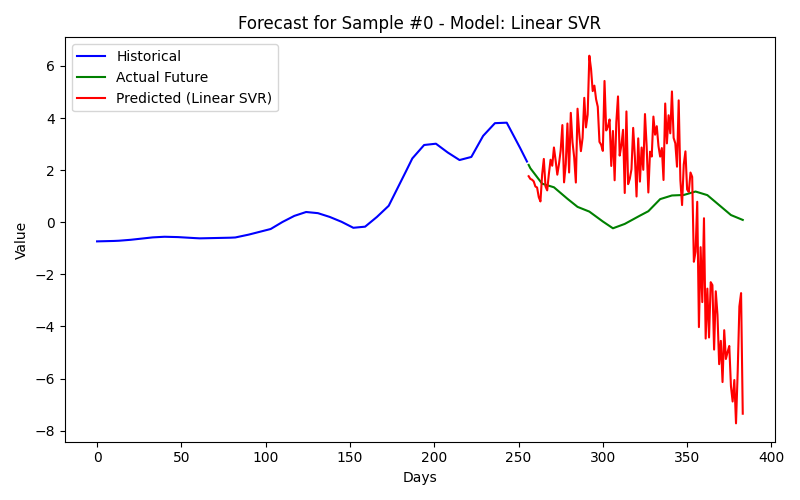
\includegraphics[width=\textwidth]{figures/regressors/Linear SVR/healthcare_256-128.png}
         \caption{Horizon 256$\to$128}
         \label{fig:SVR_healthcare_256to128}
    \end{subfigure}
    \caption{Linear SVR forecasts on the Healthcare dataset for different horizons.}
    \label{fig:SVR_healthcare_all}
\end{figure}



\chapter{Appendix: Training Configuration}\label{appendixC}

\begin{table}[h!]
\centering
\begin{tabular}{lc}
\hline
\textbf{Parameter} & \textbf{Value} \\
\hline
Optimizer & Adam \\
Batch Size & 32, 64, 128 (Optuna) \\
Learning Rate & $10^{-4}$ to $10^{-2}$ (Optuna) \\
Weight Decay & $10^{-6}$ to $10^{-3}$ (Optuna) \\
Rho & 0.3 to 0.7 (Optuna) \\
Epochs & 100 \\
Normalization & Revin \\
Objective Metric & RMSE (Optuna tuning) \\
Framework & PyTorch \\
\hline
\end{tabular}
\caption{Training Configuration for SAMFormer}
\label{tab:samformer_training}
\end{table}

\begin{table}[h!]
\centering
\begin{tabular}{lc}
\hline
\textbf{Parameter} & \textbf{Value} \\
\hline
Optimizer & - (Pretrained model) \\
Batch Size & 32, 64, 128 (Optuna) \\
Learning Rate & $10^{-5}$ to $10^{-3}$ (Optuna) \\
Horizon Length & Configurable \\
Layers & 50 \\
Positional Embedding & False \\
Checkpoint & Hugging Face (\texttt{google/timesfm-2.0-500m-pytorch}) \\
Framework & PyTorch \\
\hline
\end{tabular}
\caption{Training Configuration for TimesFM}
\label{tab:timesfm_training}
\end{table}

\begin{table}[h!]
\centering
\begin{tabular}{lc}
\hline
\textbf{Parameter} & \textbf{Value} \\
\hline
Fine-Tuning Steps & 10 \\
Fine-Tuning Depth & 5 \\
Forecasting API & Nixtla TimeGPT \\
Optimizer & Proprietary (unknown) \\
Architecture & Transformer-based (proprietary) \\
\hline
\end{tabular}
\caption{TimeGPT Model Parameters}
\label{tab:timegpt_parameters}
\end{table}

\begin{table}[h!]
\centering
\begin{tabular}{lc}
\hline
\textbf{Parameter} & \textbf{Value} \\
\hline
Optimizer & AdamW \\
Batch Size & 64 (default) \\
Learning Rate & 5e-5 (default) \\
Gradient Checkpointing & Enabled \\
Precision & FP32, FP16, BF16 \\
Framework & PyTorch \\
DeepSpeed & Enabled \\
Normalization Method & Zero, Max, None \\
Seed & 9899 \\
Scheduler & Constant, Linear, Cosine, Constant with Warmup \\
Weight Decay & 0.1 \\
\hline
\end{tabular}
\caption{Training Configuration for Time-MoE}
\label{tab:timemoe_training}
\end{table}
